\documentclass[a4paper,11pt,twoside,openright]{report}
% KOMPILOWAĆ ZA~POMOCĄ pdfLaTeXa, PRZEZ XeLaTeXa MOŻE NIE BYĆ POLSKICH ZNAKÓW

% -------------- Kodowanie znaków, język polski -------------

\usepackage[utf8]{inputenc}
\usepackage[MeX]{polski}
\usepackage[T1]{fontenc}
\usepackage[english, polish]{babel}

% Do~poprawnego odsyłania do~bibliografii i~\phantomsection
\usepackage{hyperref}

\usepackage{amsmath, amsfonts, amsthm, latexsym} % głównie symbole matematyczne, środowiska twierdzeń

\usepackage[final]{pdfpages} % inputowanie pdfa
%\usepackage[backend=bibtex, style=verbose-trad2]{biblatex}

%Dla lepszego czytania list
\usepackage{blindtext}
\usepackage{enumitem}

%Do bawienia się kolorkami w~grid
\usepackage{tikz}

\hyphenation{DICOM}

%Dodawanie pustych stron

\usepackage{afterpage}

\newcommand\blankpage{%
    \null
    \thispagestyle{empty}%
    %\addtocounter{page}{-1}%
    \newpage}

\usepackage{mathtools}

\usepackage{textcomp} %aby były stopnie

% ---------------- Marginesy, akapity, interlinia ------------------

\usepackage[inner=20mm, outer=20mm, bindingoffset=10mm, top=25mm, bottom=25mm]{geometry}


\linespread{1.5}
\allowdisplaybreaks

\usepackage{indentfirst} % opcjonalnie; pierwszy akapit z~wcięciem
\setlength{\parindent}{5mm}


%--------------------------- ŻYWA PAGINA ------------------------

\usepackage{fancyhdr}
\pagestyle{fancy}
\fancyhf{}
% numery stron: lewa do~lewego, prawa do~prawego
\fancyfoot[LE,RO]{\thepage}
% prawa pagina: zawartość \rightmark do~lewego, wewnętrznego (marginesu)
\fancyhead[LO]{\sc \nouppercase{\rightmark}}
% lewa pagina: zawartość \leftmark do~prawego, wewnętrznego (marginesu)
\fancyhead[RE]{\sc \leftmark}

\renewcommand{\chaptermark}[1]{
\markboth{\thechapter.\ #1}{}}

% kreski oddzielające paginy (górną i~dolną):
\renewcommand{\headrulewidth}{0 pt} % 0~- nie ma, 0.5 - jest linia


\fancypagestyle{plain}{% to~definiuje wygląd pierwszej strony nowego rozdziału - obecnie tylko numeracja
  \fancyhf{}%
  \fancyfoot[LE,RO]{\thepage}%
  %\fancyfoot[RO]{\thepage}
  \renewcommand{\headrulewidth}{0pt}% Line at~the header invisible
  \renewcommand{\footrulewidth}{0.0pt}
}



% ---------------- Nagłówki rozdziałów ---------------------

\usepackage{titlesec}
\titleformat{\chapter}%[display]
  {\normalfont\Large \bfseries}
  {\thechapter.}{1ex}{\Large}

\titleformat{\section}
  {\normalfont\large\bfseries}
  {\thesection.}{1ex}{}
\titlespacing{\section}{0pt}{30pt}{20pt}
%\titlespacing{\co}{akapit}{ile przed}{ile po}

\titleformat{\subsection}
  {\normalfont \bfseries}
  {\thesubsection.}{1ex}{}


% ----------------------- Spis treści ---------------------------
\def\cleardoublepage{\clearpage\if@twoside
\ifodd\c@page\else\hbox{}\thispagestyle{empty}\newpage
\if@twocolumn\hbox{}\newpage\fi\fi\fi}


% kropki dla chapterów
%\usepackage{etoolbox}
%\makeatletter
%\patchcmd{\l@chapter}
%  {\hfil}
%  {\leaders\hbox{\normalfont$\m@th\mkern \@dotsep mu\hbox{.}\mkern \@dotsep mu$}\hfill}
%  {}{}
%\makeatother

%\usepackage{titletoc}
%\makeatletter
%\titlecontents{chapter}% <section-type>
%  [0pt]% <left>
%  {}% <above-code>
%  {\bfseries \thecontentslabel.\quad}% <numbered-entry-format>
%  {\bfseries}% <numberless-entry-format>
%  {\bfseries\leaders\hbox{\normalfont$\m@th\mkern \@dotsep mu\hbox{.}\mkern \@dotsep mu$}\hfill\contentspage}% <filler-page-format>

%\titlecontents{section}
%  [1em]
%  {}
%  {\thecontentslabel.\quad}
%  {}
%  {\leaders\hbox{\normalfont$\m@th\mkern \@dotsep mu\hbox{.}\mkern \@dotsep mu$}\hfill\contentspage}

%\titlecontents{subsection}
%  [2em]
%  {}
%  {\thecontentslabel.\quad}
%  {}
%  {\leaders\hbox{\normalfont$\m@th\mkern \@dotsep mu\hbox{.}\mkern \@dotsep mu$}\hfill\contentspage}
%\makeatother



% ---------------------- Spisy tabel i~obrazków ----------------------

\renewcommand*{\thetable}{\arabic{chapter}.\arabic{table}}
\renewcommand*{\thefigure}{\arabic{chapter}.\arabic{figure}}
%\let\c@table\c@figure % jeśli włączone, numeruje tabele i~obrazki razem


% --------------------- Definicje, twierdzenia etc. ---------------


\makeatletter
\newtheoremstyle{definition}%    % Name
{3ex}%                          % Space above
{3ex}%                          % Space below
{\upshape}%                      % Body font
{}%                              % Indent amount
{\bfseries}%                     % Theorem head font
{.}%                             % Punctuation after theorem head
{.5em}%                            % Space after theorem head, ' ', or~\newline
{\thmname{#1}\thmnumber{ #2}\thmnote{ (#3)}}%  % Theorem head spec (can be~left empty, meaning `normal')
\makeatother

% ----------------------------- POLSKI --------------------------------

\theoremstyle{definition}
\newtheorem{theorem}{Twierdzenie}[chapter]
\newtheorem{lemma}[theorem]{Lemat}
\newtheorem{example}[theorem]{Przykład}
\newtheorem{proposition}[theorem]{Stwierdzenie}
\newtheorem{corollary}[theorem]{Wniosek}
\newtheorem{definition}[theorem]{Definicja}
\newtheorem{remark}[theorem]{Uwaga}



% ----------------------------- Dowód -----------------------------

%\makeatletter
%\renewenvironment{proof}[1][\proofname]
%{\par
%  \vspace{-12pt}% remove the space after the theorem
%  \pushQED{\qed}%
%  \normalfont
%  \topsep0pt \partopsep0pt % no~space before
%  \trivlist
%  \item[\hskip\labelsep
%        \sc
%    #1\@addpunct{:}]\ignorespaces
%}
%{%
%  \popQED\endtrivlist\@endpefalse
%  \addvspace{20pt} % some space after
%}
%
%\renewcommand{\qedhere}{\hfill \qedsymbol}
%\makeatother


% --------------------------Obrazy-----------------------------

%Path relative to~the .tex file containing the \includegraphics command

\usepackage{graphicx}
\graphicspath{ {./images/} }


% -------------------------- POCZĄTEK --------------------------


% --------------------- Ustawienia użytkownika ------------------

\newcommand{\tytul}{Interfejs użytkownika do~manualnego obrysu struktur oraz wybranych anormalności w~obrazach medycznych z~wykorzystaniem tabletu graficznego}
\renewcommand{\title}{User interface for graphic-tablet interactions for contouring of~structures and selected anormalies in~medical images}
\newcommand{\type}{inżyniers} % magisters, licencjac
\newcommand{\supervisor}{dr inż. Magdalena Jasionowska}



\begin{document}
\sloppy


\includepdf[pages=-]{titlepage}


% ---------------------------- ABSTRAKTY -----------------------------
% W~PRACY PO~POLSKU, NAPIERW STRESZCZENIE PL, POTEM ABSTRACT EN

{
\begin{abstract}

%\begin{center}
%\tytul
%\end{center}
Niniejszy dokument prezentuje pracę dyplomową inżynierską pod tytułem "\tytul".
Celem realizowanym przez autorów pracy było stworzenie narzędzia do~manualnego
i~półautomatycznego obrysowywania struktur anatomicznych, zmian patologicznych
na~obrazach medycznych, wykorzystywanego zarówno przez lekarzy, jak i~inżynierów
biomedycznych.
Zakres pracy obejmuje omówienie: standardu DICOM, przegląd aplikacji dostępnych
na rynku, pozwalających na~przeglądanie i~wykonywanie obrysów na~obrazach
medycznych DICOM, architektury tworzonego systemu i~eksperymentów przeprowadzonych
w trakcie tworzenia zaproponowanego narzędzia.

Zastosowana architektura umożliwia jednoczesne korzystanie z~narzędzia przez
wielu użytkowników. Moduł obrysów manualnych został zaimplementowany głównie
w~warstwie ściśle związanej z~interfejscem użytkownika. Moduł obrysów półautomatycznych
bazuje na~algorytmie opracowanym na~potrzeby generowania obrysów, który wykorzystuje
operator Canny'ego oraz algorytm wyszukiwania najkrótszych ścieżek w~grafie.
Dodatkowo dodany moduł statystyczny umożliwia wyznaczenie podstawowych miar statystycznych,
opisujących obrysowane fragmenty obrazów.
\\
\\
\noindent \textbf{Słowa kluczowe:} interfejs użytkownika, tablet graficzny, obrazy medyczne, DICOM, obrys, statystyki danych obrazowych, system informatyczny, interfejs REST API, wykrywanie krawędzi, generowanie obrysów
\end{abstract}
}

\null\thispagestyle{empty}\newpage

{
\selectlanguage{english}
\begin{abstract}

%Nie przetłumaczyłem

Do nowego przetłumaczenia - Tomek.

%The following document describes bachelor's thesis on~"\title". The goal of~authors' is~to~create a~digital tool that allows to~manually draw and semi-automatically generate contours on~medical images. The topics discussed include: discussion of~DICOM standard, analysis of~state-of-the-art systems and tools used to~viewing and creating contours on~DICOM medical images, system's architectue and experiments conducted simultaneously with the creation of~the tool.

%The architecture used enables simultaneous use of~the tool by~many users. The algorithm developed for te~purpose of~generating contourse uses Canny's Operator and the algorithm of~searching the shortest path in~the graph. The statistics calculated by~the system regarding the areas limited by~contourcan be~used in~future as~input parameters for methods of~automatic detection of~similar structures for which contours have been made.
%\\
%\\
\noindent \textbf{Keywords:} user interface, graphics tablet, medical images, DICOM, contour, statistics of~image data, IT~system, REST API interface, edge detection, contour generation
\end{abstract}
}


% --------------------- OŚWIADCZENIE -----------------------------------------


\null\thispagestyle{empty}\newpage

\null \hfill Warszawa, dnia ..................\\

\par\vspace{5cm}

\begin{center}
Oświadczenie
\end{center}

\indent Oświadczam, że moją część pracy \type kiej
(zgodnie z~podziałem zadań opisanym we~wstępie) pod
tytułem ,,\tytul '', której promotorem jest \supervisor , wykonałem
samodzielnie, co~poświadczam własnoręcznym podpisem.
\vspace{2cm}


\begin{flushright}
  \begin{minipage}{50mm}
    \begin{center}
      ..............................................

    \end{center}
  \end{minipage}
\end{flushright}

\thispagestyle{empty}
\newpage

\null\thispagestyle{empty}\newpage


% ------------------- 4. Spis treści ---------------------
\pagenumbering{gobble}
\tableofcontents
\thispagestyle{empty}

%\newpage % JEŻELI SPIS TREŚCI MA~PARZYSTĄ LICZBĘ STRON, ZAKOMENTOWAĆ
% ALBO JAK KTOŚ WOLI WTEDY DWIE STRONY ODSTĘPU, DODAĆ \null\newpage

% -------------- 5. ZASADNICZA CZĘŚĆ PRACY --------------------
\null\thispagestyle{empty}\newpage
\pagestyle{fancy}
\pagenumbering{arabic}
\setcounter{page}{11} % JEŻELI Z~POWODU DUŻEJ ILOŚCI STRON W~SPISIE TREŚCI SIĘ NIE ZGADZA, TRZEBA ZMODYFIKOWAĆ RĘCZNIE
%oryginalnie było 11
%ustawiam ponownie 11, usunąłem pustą stronę po~spisie treści - rodziały powinny zaczynać się na~stronach nieparzystych

\chapter*{Wstęp}
\markboth{}{Wstęp}
\addcontentsline{toc}{chapter}{Wstęp}

W niniejszym rozdziale przedstawiono cel pracy inżynierskiej wraz z~motywacją,
która kierowała autorami przy wyborze właśnie tego tematu.

\section*{Motywacja}

W czasach gwałtownego rozwoju sztucznej inteligencji jest ona stosowana prawie
do każdej dziedziny z~szeroko pojętej nauki. Jedną z~takich dziedzin jest także medycyna.
Powstają coraz to nowsze rozwiązania komputerowego wspomagania medycyny w diagnostyce i~terapii.
Jednym z takich zagadnień jest próba rozpoznawania we~wczesnym stadium różnych zmian
patologicznych na obrazach medycznych. Wczesne wykrywanie zmian pozwala
na~szybką terapię, a~w~konsenkwencji niejednokrotnie na~całkowite wyleczenie. Między innymi dlatego
tak ważne jest tworzenie komputerowych systemów wspomagania procesu podejmowania
decyzji przez radiologów w~diagnostyce obrazowej.

Komputerowe wspomaganie diagnostyki obrazowej może dotyczyć między innymi automatycznej
detekcji zmian patologicznych uwidocznionych na~obrazach (np. systemy CAD stosowane
w~mammografii) lub nieuwidocznionych (np. rozpoznanie udaru niedokrwiennego na~obrazach %cite!!!!!!!!!!!!!!!!!!!!!!!!!!!!!!!!!!!!!!!!!!!!!!!!!!!!!!!!!!!!!!!!!!!!!!!
CT we~wczesnej fazie). W~celu stworzenia dobrego narzędzia automatycznego wspomagania %cite!!!!!!!!!!!!!!!!!!!!!!!!!!!!!!!!!!!!!!!!!!!!!!!!!!!!!!!!!!!!!!!!!!!!!!!
decyzji należy posiadać zbiór danych referencyjnych. W~praktyce wykorzystuje się
dane obrazowe opisane i obrysowane przez lekarzy---specjalistów. Ten etap prac
jest czasochłonny i żmudny. Dlatego warto automatyzować ten etap tworzenia narzędzi
komputerowego wspomagania decyzji.

\section*{Cel pracy}

Celem niniejszej pracy inżynierskiej było stworzenie narzędzia informatycznego,
umożliwiającego tworzenie obrysów zarówno struktur anatomicznych, jak i~zmian patologicznych
na~obrazach medycznych. Użytkownik może otwierać
dane obrazowe w~formacie DICOM i~dokonywać obrysów manualnych lub półautomatycznych
wybranych struktur lub anormalności. W~przypadku obrysów manualnych użytkownik
może tworzyć kilka obrysów jednocześnie w~celu zaznaczania anormalności w~obrazowanej tkance.
Użytkownik może korzystać z~tabletu graficznego w~celu wygodniejszego rysowania obrysów.

W ramach pracy stworzono także algorytm do~tworzenia obrysów półautomatycznych.
Metoda ta polega na wybraniu przez użytkownika punktów na~obrazie, a~następnie
wygenerowaniu obrysów z~uwzględnieniem tych punktów. W~tym celu
został użyty operator Canny'ego, a~następnie punkty przetwarzane są
poprzez algorytmy grafowe.
%Została przeprowadzona walidacja,
%czy ta~metoda sprawdza się w~celu usprawnienia rysowania obrysów manualnych. @Tomek ??????????????????????????????????????

Z zaproponowanego przez autorów rozwiązania mogą korzystać lekarze w~codziennej pracy, ale także
studenci medycyny w~celu nauki wykrywania zmian patologicznych, czy też lekarze i~inżynierowie
biomedyczni w~trakcie współpracy w~badaniach naukowych.

Zaproponowane przez autorów rozwiązanie opiera się na~aplikacji przeglądarkowej
i~na~serwerze przechowującym obrysy. To~rozwiązanie pozwala na~użycie go~w~sieciach
lokalnych, gdzie użytkownik lub użytkownicy na~dowolnej stacji roboczej mogą
wykonywać obrysy, które zapisywane są na~wspólnym dla wszystkich użytkowników serwerze.


\chapter {Wprowadzenie}

W tym rozdziale zostało przedstawione wprowadzenie dotyczące formatu obrazów
medycznych DICOM i~aspektu medycznego pracy.
Ponadto opisano podział prac wykonanych w~trakcie tworzenia
narzędzia informatycznego.

\section {Zagadnienia medyczne}

DICOM (ang. Digital Imaging and Communications in~Medicine) \cite{DICOM} to~norma
opracowana dla potrzeb wymiany i~interpretacji danych medycznych, które są
najczęściej obrazami medycznymi. W~postaci pliku DICOM mogą być zapisywane obrazy
tomografii komputerowej, obrazowania metodą rezonansu magnetycznego, cyfrowej
angiografii subtrakcyjnej, zdjęcia rentgenowskie, mammografia i~wiele innych badań.
Do wad tego standardu należy różnorodność metod implementacji, co powoduje to~czasem
sytuacje, w~których nie można wyświetlić pliku na~sprzęcie innego producenta.
W~takich sytuacjach należy ręcznie
modyfikować badania, aby mogły być poprawnie obsłużone. Ponadto liczba tagów zawartych w~badaniu
DICOM stanowi barierę w~sprawnym korzystaniu z~tak zapisanych wyników badań.

\section {Automatyczna detekcja zmian patologicznych}

Na~podstawie wyników badań zapisanych w~formacie DICOM lekarze są~w~stanie diagnozować
pacjentów i~wybierać terapię odpowiednią dla zauważonych w~badaniu nieprawidłowości.
W~celu ułatwienia odpowiedniej diagnozy jak również weryfikacji oceny lekarza
przydatne są narzędzia automatycznej detekcji zmian patologicznych,
które służą do~przetwarzania danych obrazowych w~celu
wykrycia patologicznych zmian. Wykorzystują do~tego między innymi metody sztucznej
inteligencji, które do poprawnego działania wymagają zbioru testowego --- zbioru
obrysów zmian patologicznych. Na podstawie tego zbioru algorytm uczy się
wykrywać podobne zmiany w badaniach poddawanych automatycznej detekcji.
Ze~względu na~to~kluczowe znaczenie dla poprawności decyzji algorytmu ma~dokładność zbioru testowego.

\section {Obrysy zmian patologicznych}

Dokładność obrysu w~dużym stopniu zależy od~rozdzielczości badania obrazowego i~precyzji
wyboru punktów przez użytkownika. Obrys powinien znajdować się na krawędzi
obrysowywanej tkanki, co jest bardzo trudne do uzyskania manualnie,
dlatego pomocne mogą być algorytmy wykrywania krawędzi na obrazie, które pozwalają one na automatyczne
wykrycie kształtów struktur znajdujących się na obrazie. Zastosowanie takich algorytmów
pozwala na~zwiększenie precyzji obrysów wykonywanych manualnie oraz na~skrócenie
czasu wykonywania pojedynczego obrysu.

Na rynku istnieją już rozwiązania umożliwiające wykonywanie obrysów,
zarówno manualnie (np. ImageJ) jak również z automatycznym wykrywaniem krawędzi (np. DWV).
Wspomniane narzędzia zwykle nie dają możliwości wykonywania obrysów wieloma metodami,
a jedynie na obrysy manualne albo półautomatyczne. Ponadto często mają skomplikowany
interfejs, który stanowi spore utrudnienie w korzystaniu przez użytkowników.

\section {Proponowane rozwiązanie}

W celu usprawnienia procesu tworzenia obrysów zmian patologicznych przygotowane
zostało narzędzie pozwalające na~wykonywanie obrysów dwiema metodami:
manualną i~półautomatyczną. Ponadto narzędzie pozwala~na zapisywanie wykonanych obryów,
obliczanie statystyk dotyczących regionu zainteresowania oraz anonimizację badań DICOM.
Narzędzie działa w przeglądarce internetowej i~pozwala na wykonywanie obrysów na badaniach
zapisanych na zdalnym serwerze.

\section {Podział prac}

Ze względu na~złożoność realizowanego narzędzia dokonano podziału zadań pomiędzy
członków zespołu.

Łukasz Garstecki wykonał:

\begin{itemize}[noitemsep]
	\item moduł obrysów manualnych,
	\item moduł anonimizacji,
	\item interfejs wyświetlania wykonanych obrysów.
\end{itemize}

\pagebreak

Tomasz Świerczewski wykonał:

\begin{itemize}[noitemsep]
\item moduł obrysów półautomatycznych,
\item moduł statystyk,
\item moduł zapisu obrysów.
\end{itemize}

\afterpage{\blankpage}

\chapter {Stan wiedzy}

W poniższym rozdziale zostały przedstawione istniejące na~rynku aplikacje o
funkcjonalnościach określonych w~celu niniejszej pracy. Opisano zarówno funkcjonalne jak i~niefunkcjonalne
wymagania dla projektowanego systemu. Zaproponowany system do~tworzenia obrysów
na obrazach w~formacie DICOM struktur anatomicznych czy zmian patologicznych
powinien spełniać wymagania zarówno lekarzy, jak i~inżynierów medycznych, wykorzystujących
to narzędzie w~pracy badawczej i~naukowej. Przedstawiono również proponowane rozwiązanie
postawionych wymagań.

\section {Przegląd istniejących rozwiązań}

Obrysy to~krzywe zamknięte naniesione na~obraz w~celu oznaczenia wewnętrznej części
regionu zainteresowania (ang. \textit{ROI --- region of interest}).
Obrysy można tworzyć manualnie (użytkownik wybiera wszystkie punkty obrysu) lub
półautomatycznie (użytkownik wybiera kilka punktów, a~algorytm łączy je~przy wykorzystaniu
algorytmu Canny'ego). Obrysy tworzone obiema metodami są modyfikowalne przez użytkownika,
co w takich zastosowaniach jak obrysy na obrazach medycznych ma duże znaczenie. Użytkownik często musi skorygować
wygenerowany obrys ze~względu na~różnorodność obrazów medycznych wynikających z~różnych systemów
obrazowania, czy też ze~względu na~różnorodność tekstury tkanki obrazowanej (innej dla każdego pacjenta).

\subsection {Przeglądarki DICOM}

Istnieje wiele rozwiązań umożliwiających wykonywanie obrysów przy użyciu przeglądarki.
W~tej pracy opisano szczegółowo dwie wybrane aplikacje, które według autorów w~największym
stopniu spełniają założone cele pracy.

Pierwsza z~nich to~aplikacja OHIF Viewer \cite{OHIF Viewer} oparta o~biblioteki Cornerstone.

Cornerstone Core \cite{Cornerstone Core} to~biblioteka, która umożliwia przetwarzanie
obrazów medycznych z~wykorzystaniem elementu canvas z~języka HTML5. Biblioteka
udostępnia interfejs do~wyświetlania obrazów medycznych pozwalający na~zarządzanie
wyświetlaniem obrazu. Podstawowe funkcjonalności obsługiwane przez tę bibliotekę to:

\begin{itemize}[noitemsep]
\item przybliżanie i~oddalanie obrazu,
\item obrót obrazu,
\item przesuwanie obrazu na ekranie,
\item zmiana jasności wyświetlanego obrazu,
\item mapowanie kolorów,
\item interpolacja pikseli w~obrazie (dla obrazów o~niskiej rozdzielczości).
\end{itemize}

Ponadto twórcy biblioteki Cornerstone Core stworzyli bibliotekę Cornerstone Tools \cite{Cornerstone Tools},
która korzysta z~biblioteki Cornerstone Core i~poza funkcjonalnościami
Cornerstone Core udostępnia opisane niżej funkcjonalności
potrzebne lekarzom do~analizy badań pacjentów, takie jak:

\begin{itemize}[noitemsep]
\item mierzenie odległości w~linii prostej na~obrazie z~podaniem rzeczywistych wartości,
\item oznaczanie obszarów przy pomocy prostokątów oraz elips,
\item oznaczanie niewielkich zmian w~postaci małego okręgu,
\item mierzenie kątów na~podstawie trzech podanych przez użytkownika punktów.
\end{itemize}

Przykładowym projektem korzystającym z~bibliotek Cornerstone jest OHIF Viewer.
Aplikacja pozwala na~wykorzystanie większości możliwości udostępnianych przez
biblioteki Cornerstone. Przykładowe użycie aplikacji zostało przedstawione na
Rysunku \ref{fig:OHIF-example}.

\begin{figure}[b!]
	\center
	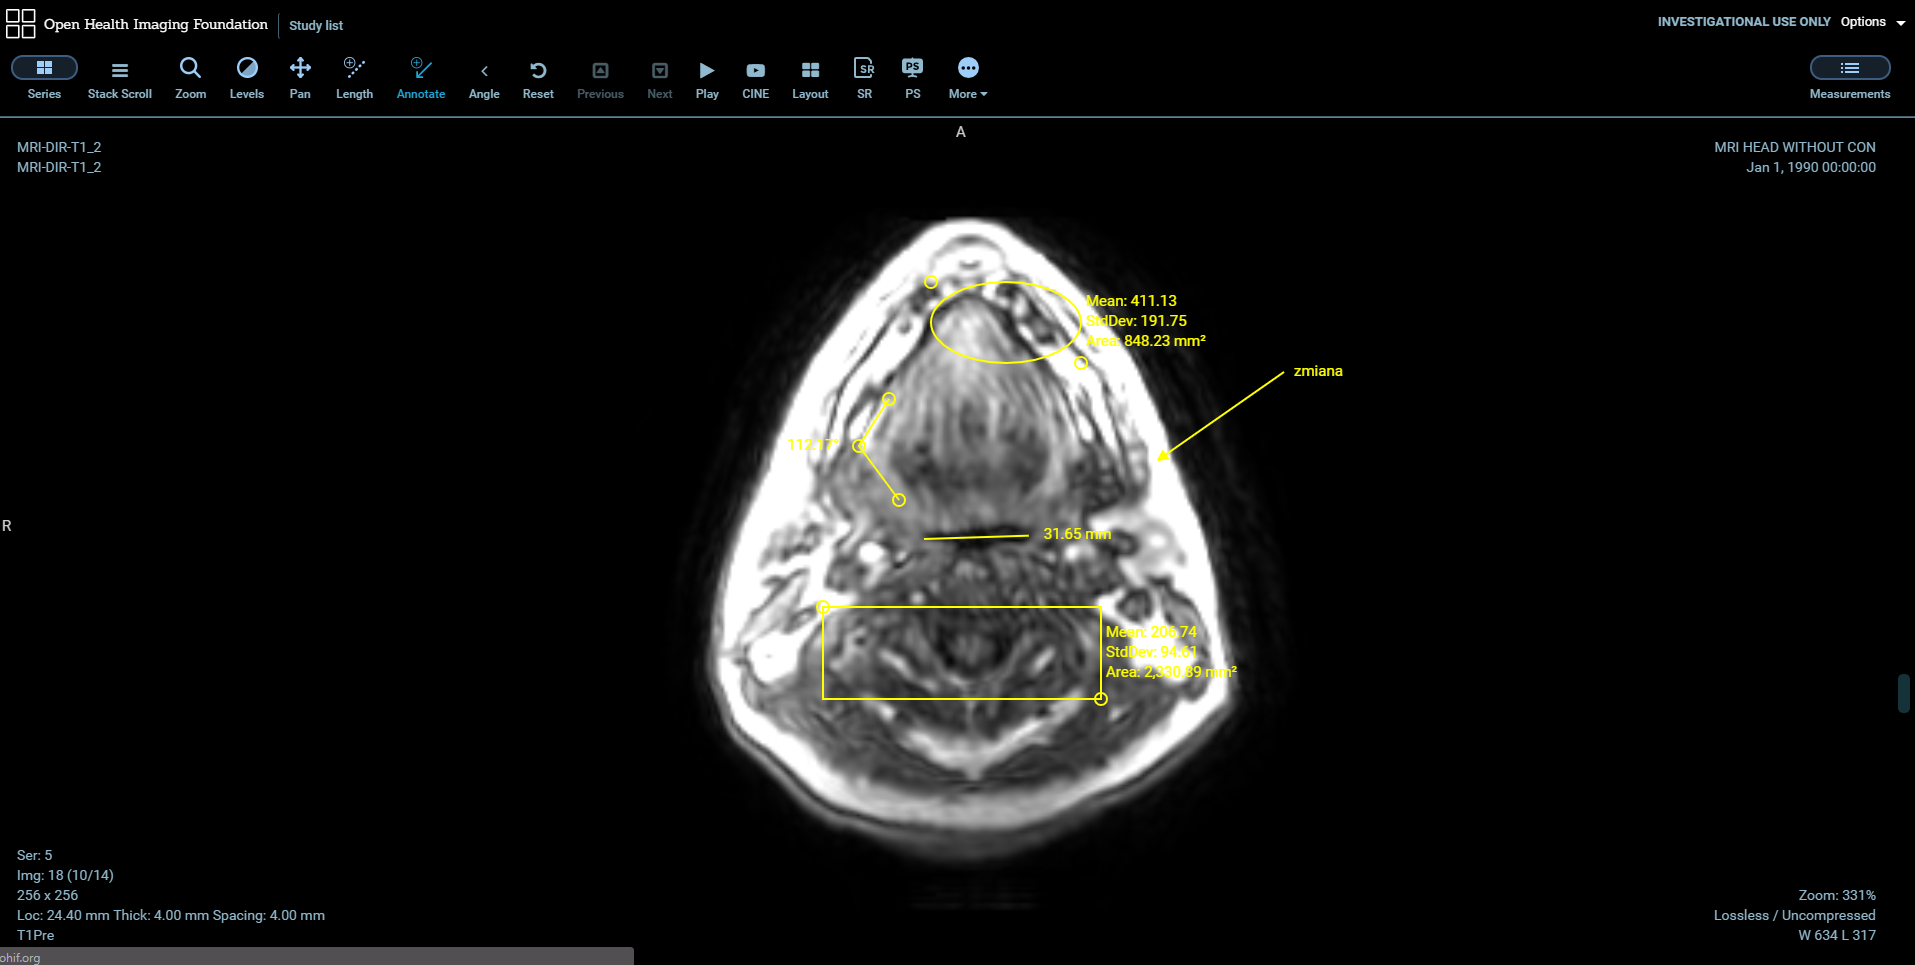
\includegraphics[width=0.7\textwidth]{OHIF-example}
	\caption{Przykład użycia aplikacji OHIF Viewer --- oznaczono: prostokątny obszar,
	dla którego obliczone zostały wybrane statystyki; odcinek, dla którego otrzymano
	odległość w~jednostkach rzeczywistych; wskaźnik, wskazujący na~zmianę i posiadający
	etykietę tekstową.}
    	\label{fig:OHIF-example}
\end{figure}

Niestety aplikacja OHIF Viewer nie umożliwia wykonywania obrysów manualnych ani półautomatycznych,
jak również nie pozwala na~zapisanie naniesionych na~obraz oznaczeń.

Drugim rozwiązaniem działającym i~pozwalającym na~pracę z~plikami DICOM w~przeglądarce
internetowej jest DICOM Web Viewer \cite{DWV}.

Aplikacja DICOM Web Viewer (DWV) jest również przykładem aplikacji
przeglądarkowej służącej do~przetwarzania obrazów DICOM, z~wygodnym interfejsem
automatycznego i~półautomatycznego obrysowywania obszarów zaznaczonych
przez użytkownika na~obrazie. Przykładowy obrys wykonany przy użyciu aplikacji
DWV przedstawiono na~Rysunku \ref{fig:DWV-interface}.

\begin{figure}[tb!]
	\center
	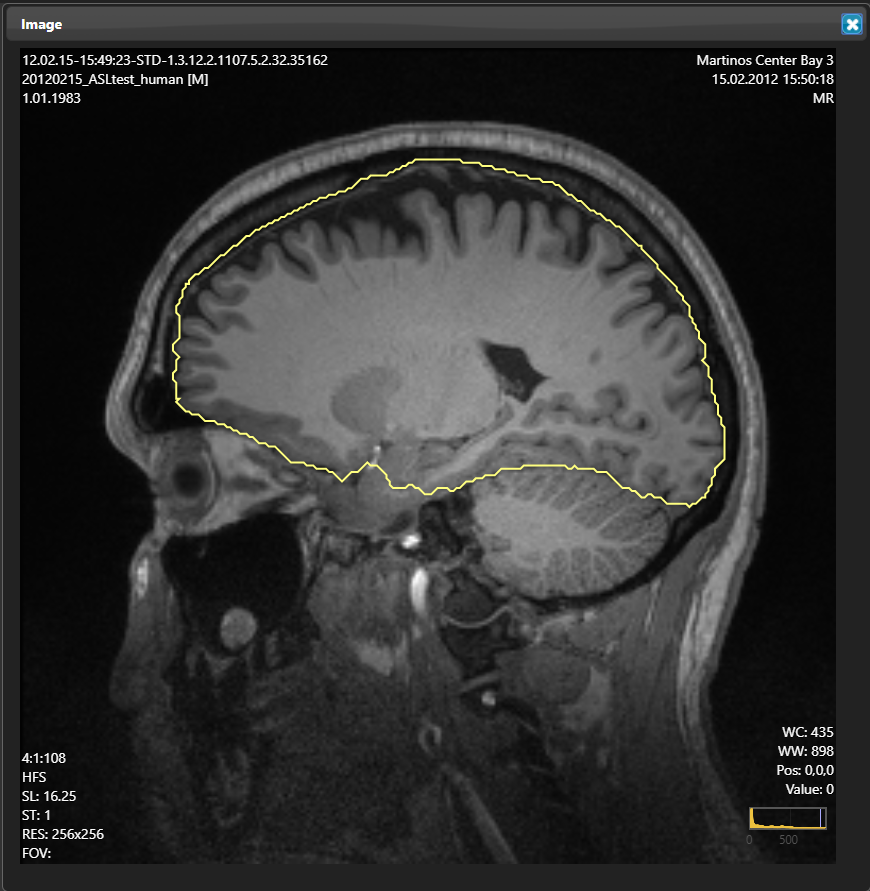
\includegraphics[width=0.7\textwidth]{DWV-interface}
	\caption{Przykład użycia aplikacji DWV - obrys półautomatyczny (Livewire) \cite{DWV}}
    	\label{fig:DWV-interface}
\end{figure}

 Poza tym aplikacja udostępnia:
\begin{itemize}[noitemsep]
\item przybliżanie i~oddalanie obrazu,
\item przesuwanie obrazu w~wyświetlanym komponencie,
\item możliwość zmiany jasności wyświetlanego obrazu,
\item mierzenie odległości w~linii prostej na~obrazie z~podaniem rzeczywistych wartości,
\item oznaczanie obszarów przy pomocy prostokątów oraz elips.
\end{itemize}

Aplikacja nie pozwala na~wykonywanie manualnych obrysów poprzez samodzielne
poruszanie kursorem po~obrazie.

\subsection {Serwer z~bazą plików DICOM}

Orthanc \cite{Orthanc} to~serwer plików DICOM, który umożliwia łatwe przechowywanie,
zarządzanie oraz dostęp do~plików medycznych DICOM. Ponadto Orthanc udostępnia
REST API \cite{Orthanc API}, które umożliwia przeglądanie wgranych na~serwer plików DICOM podzielonych
na kategorie takie jak: dane pacjentów, badania pacjenta i~serie.

Serwer Orthanc udostępnia prosty interfejs webowy, dzięki któremu możliwe jest
wgrywanie nowych plików (interfejs wgrywania plików przedstawiono na~Rysunku
\ref{fig:Orthanc-upload}), przeglądanie zapisanych plików w~szczególności
tagów (Rysunek \ref{fig:Orthanc-tags}) oraz podglądanie obrazów (Rysunek \ref{fig:Orthanc-preview}).
Interfejs webowy nie zapewnia żadnej metody tworzenia na~wybranym obrazie, ale
pozwala na~przełączanie pomiędzy kolejnymi obrazami za~pomocą kliknięcia lewym
przyciskiem myszy w~prawą część podglądu obrazu.

\begin{figure}[tb!]
	\center
	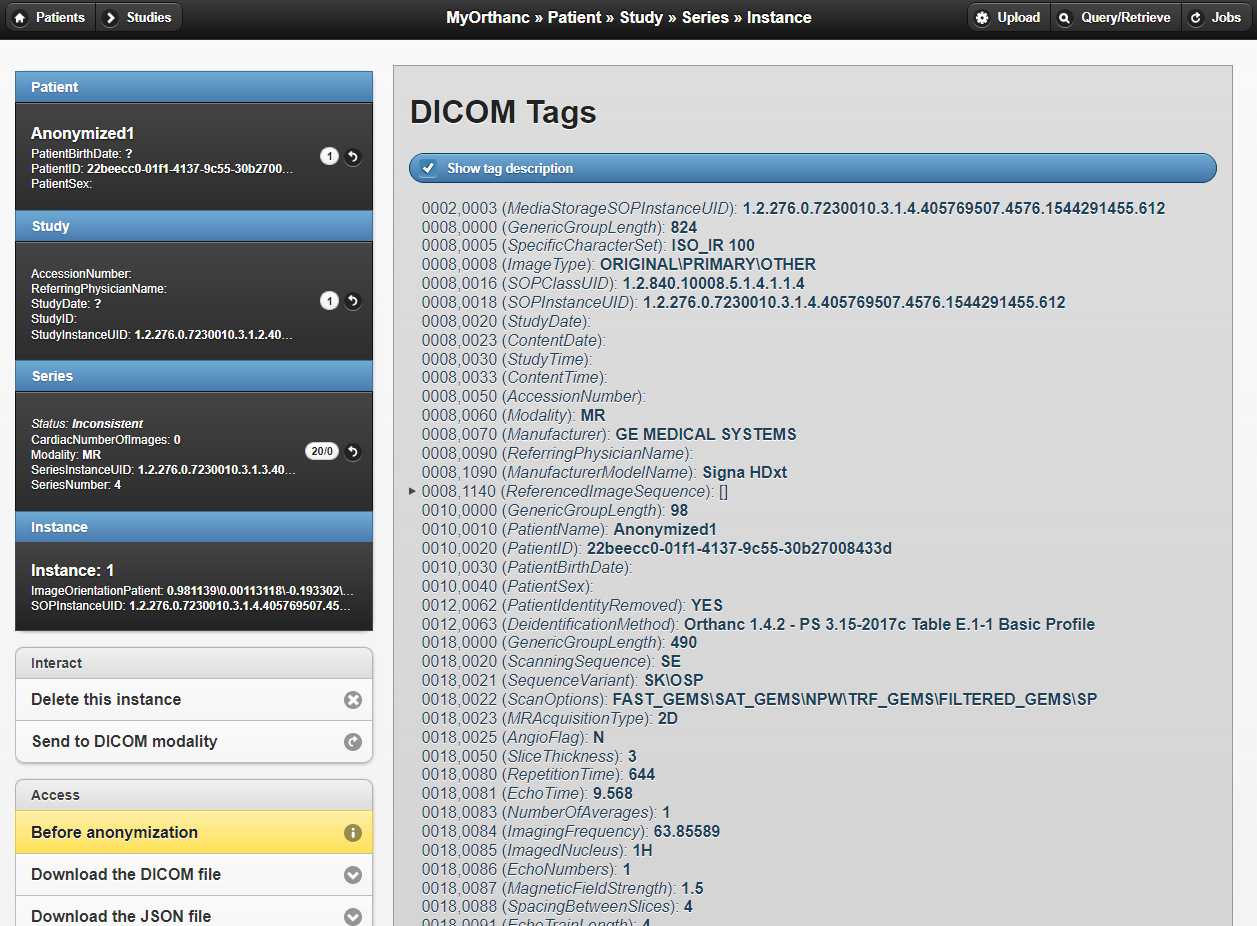
\includegraphics[width=0.95\textwidth]{Orthanc-tags}
	\caption{Podgląd tagów pliku DICOM przy użyciu interfejsu przeglądarkowego Orthanc}
    	\label{fig:Orthanc-tags}
\end{figure}

\begin{figure}[tb!]
	\center
	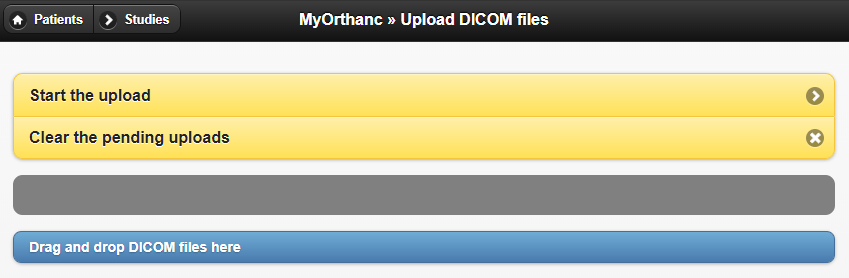
\includegraphics[width=0.8\textwidth]{Orthanc-upload}
	\caption{Interfejs wgrywania plików DICOM do~serwera Orthanc \cite{Orthanc}}
    	\label{fig:Orthanc-upload}
\end{figure}

\begin{figure}[tbh!]
	\center
	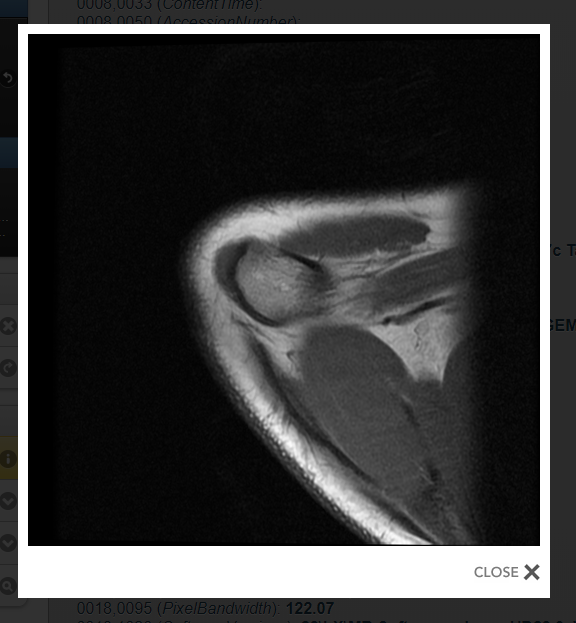
\includegraphics[width=0.55\textwidth]{Orthanc-preview}
	\caption{Podgląd obrazu DICOM przy użyciu interfejsu przeglądarkowego Orthanc}
    	\label{fig:Orthanc-preview}
\end{figure}

Innym rozwiązaniem pozwalającym na zarządzanie badaniami obrazowymi jest SonicDICOM~\cite{SonicDICOM}.
Podobnie jak Orthanc udostępnia on API \cite{SonicDICOM API}, pozwalające na komunikację zewnętrznych narzędzi
z systemem w celu przeglądania, wyświetlania i modyfikacji zapisanych w systemie badań.

Analogicznie jak Orthanc, SonicDICOM posiada wbudowany interfejs do przeglądania
zapisanych w systemie badań, który nie umożliwia wykonywania obrysów na badaniach.

\begin{figure}[tb!]
	\center
	\includegraphics[width=0.6\textwidth]{SoniCDICOMViewer}
	\caption{Podgląd obrazu DICOM przy użyciu interfejsu SonicDICOM \cite{SonicDICOM API}}
    	\label{fig:SonicDICOM}
\end{figure}

System SonicDICOM jest rozwiązaniem komercyjnym i wykorzystanie go wymaga wykupienia
licencji w celu korzystania z zawartych w nim funkcjonalności.

\subsection {Podsumowanie}

Wymienione rozwiązania przeglądarkowe nie zapewniają wygodnego interfejsu użytkownikowi
do manualnego obrysowywania interesujących go~fragmentów obrazów medycznych przy użyciu tabletu graficznego.
Ponadto żadne z~tych narzędzi nie przechowuje obrysów utworzonych w~sposób manualny
ani półautomatyczny.

\section {Proponowane rozwiązanie}

Przygotowane rozwiązanie zapewnia funkcjonalności niedostępne w innych narzędziach
takie jak: połączenie funkcjonalności manualnego i półautomatycznego generowania obrysów,
zapisanie i przeglądanie wykonanych i wygenerowanych obrysów,
obliczanie statystyk związanych z wykonanymi obrysami, jak również zmiana danych pacjenta
dla przeglądanego badania.

W zaproponowanym rozwiązaniu (Rysunek \ref{fig:architektura2}) zdecydowano się skorzystać z~serwera Orthanc jako bazy przechowującej
pliki DICOM. Przy decyzji miało znaczenie przede wszystkim to, że jest to~narzędzie
bezpłatne. Ponadto udostępniane przez API serwera funkcjonalności pozwalające na
zarządzanie i~przeglądanie zapisanych plików były wystarczające dla realizowanego systemu.

Poza serwerem Orthanc stworzono serwer w~technologii .NET Core \cite{Dotnet}
wspomagający interfejs użytkownika, który pozwala na~przeprowadzanie czasochłonnych
aplikacji poza interfejsem użytkownika. Wybrano tę technologię ze~względu na~to,
że jest ciągle rozwijana, podobnie jak Orthanc .NET Core jest rozwiązaniem darmowym
i nie ustępuje jakością w~stosunku do~Java~EE~\cite{Dlaczego dotnet}.
Podstawowymi zadaniami tego serwera było przechowywanie
wykonanych przez użytkownika obrysów manualnych, generowanie i~przechowywanie
obrysów półautomatycznych oraz obliczanie statystyk związanych z~zapisanymi obrysami.

Jako interfejs użytkownika wykorzystano bibliotekę ReactJS \cite{React} w~połączeniu
z biblioteką Redux\cite{Redux}. Zdecydowano się na~tę technologię ze~względu na~bardzo dobre wsparcie techniczne
i elastyczność \cite{Dlaczego react}. Wybranie tej technologii pozwoliło na~stworzenie
aplikacji przeglądarkowej, pozwalającej na~generowanie obrysów manualnych przy
użyciu myszy lub tabletu graficznego, wybieranie punktów, z~których generowane
będą obrysy półautomatyczne, możliwość oglądania wcześniej wygenerowanych i~zapisanych
obrysów oraz wyświetlanie statystyk dotyczących wykonanego obrysu. Interfejs
inspirowany jest podglądem obrazu w~aplikacji DWV, ale działanie półautomatycznego
obrysu zostało zrealizowane inaczej --- obrys nie jest generowany na~bieżąco, lecz na~życzenie
użytkownika. Wybrane przez niego punkty na~obrazie wysyłane są do~serwera i~na~obrazie wyświetlany jest
wynik półautomatycznego dopasowania obrysu.

\begin{figure}[tb]
	\center
	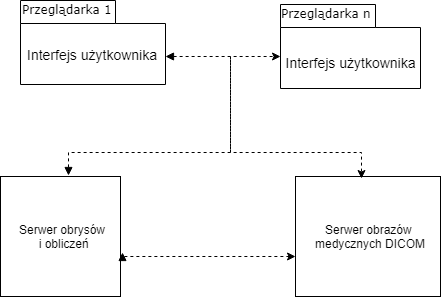
\includegraphics[width=0.7\textwidth]{architektura2}
	\caption{Diagram przedstawiający części autorskiego systemu}
    	\label{fig:architektura2} % TODO: add image!!!!!!!!!!!!!!!!!!!!!!!!!!!!!!!!!!!!!!!!!!!!!!!
\end{figure}

\afterpage{\blankpage}

\chapter {Opis autorskiego narzędzia informatycznego}

W poniższym rozdziale zawarto dokumentację biznesową, jak i~techniczną tworzonego narzędzia.
Przedstawiono wymagania funkcjonalne i~niefunkcjonalne,
architekturę narzędzia, a także zastosowane metody półautomatycznego obrysu oraz metody obliczania
statystyk dla wybranego obszaru obrazu wewnątrz obrysu.

\section {Specyfikacja wymagań}

Specyfikacja wymagań została opracowana na podstawie danych dotyczących wymagań stawianych
przed tworzonym systemem. Zostały one przedstawione w~rozdziałach 3.1.1. - 3.1.3. Wymagania
były konsultowane %z~lekarzami i~studentami ostatniego roku medycyny z Warszawskiego Uniwersytetu Medycznego.
środowiskiem medycznym m.in. Warszawskim Uniwersytetem Medycznym.

\subsection {Opis biznesowy}
\interfootnotelinepenalty=10000

Celem projektu było stworzenie interfejsu przyjaznego użytkownikowi, który umożliwi
przeglądanie obrazów DICOM, w~celu wykonywania obrysów na~tych obrazach, a~także wyliczenia
statystyk dotyczących wykonanych obrysów. Praca
obejmowała stworzenie aplikacji webowej, która udostępni użytkownikowi interfejs
komunikujący się z~bazą danych Orthanc. Ponadto praca obejmowała stworzenie serwera
odpowiedzialnego za~przechowywanie wygenerowanych przez użytkownika obrysów oraz
wyznaczanie obrysów półautomatycznych.

Do podstawowych funkcjonalności systemu zaliczają się:
\begin{itemize}[noitemsep]
%O listach wyliczeniowych https://sjp.pwn.pl/poradnia/haslo/listy-wyliczeniowe;4812.html
\item anonimizacja\footnote {Anonimizacja (ang. anonymization) --- operacja mająca
na celu usunięcie z~danych informacji o~pacjentach, które pozwoliłyby na~identyfikację
danych z~tożsamością pacjenta. Są to~między innymi: imiona, nazwisko, pesel.
Inne tłumaczenia słowa anonymization --- utajnianie, usuwanie danych niejawnych.
Z uwagi na~fakt, że te~tłumaczenia nie oddają dobrze kontekstu, zastosowano kalkę
językową.} danych zapisanych w~strukturze pliku DICOM, w~sytuacji braku takiej anonimizacji,
\item generowanie obrysu manualnego,
\item generowanie obrysu półautomatycznego na~podstawie punktów wybranych przez użytkownika,
\item zapisywanie wygenerowanych obrysów w postaci plików CSV zawierających
punkty wybrane przez użytkownika i wyliczone statystyki.
\end{itemize}

\subsection {Wymagania funkcjonalne}

Nieodłącznym elementem inżynierii oprogramowania przy tworzeniu dokumentacji
określonego produktu lub usługi, są wymagania funkcjonalne i~niefunkcjonalne.
Te pierwsze opisują funkcje i~możliwości, które system powinien realizować, drugie
natomiast mówią o tym jakiej wydajności, użyteczności i dostępności wymaga się od tworzonego narzędzia.
Wymagania funkcjonalne dla tworzonego systemu zostały przygotowane na podstawie
konsultacji z~lekarzami i studentami ostatniego roku radiologii. Przedstawiono
je poniżej w~postaci historii użytkownika (ang. user stories), czyli czynności
jakie może chcieć wykonać użytkownik tego systemu.
\begin{enumerate}
\item \textbf {Jako użytkownik chcę wczytać obraz DICOM.} \\
Użytkownik może wybrać obraz w~menu bocznym, w~którym ma~możliwość wyboru pacjenta,
badania oraz serii. Wybranie serii skutkuje wyświetleniem pierwszego obrazu DICOM z~tej serii.

\item \textbf {Jako użytkownik chcę zmienić obraz w~serii przy użyciu rolki myszy.} \\
Po umieszczeniu kursora na~obrazie, przewijanie rolką myszy do~góry powoduje zmianę
wyświetlanego obrazu na~kolejny obraz w~serii. Gdy rolka myszy jest przewijana do~góry
na ostatnim obrazie w~serii wyświetlany obraz nie zmienia się. Analogicznie
przewijanie rolką myszy w~dół powoduje zmianę wyświetlanego obrazu na~poprzedni
obraz w~serii, a~przewijanie w~dół rolką myszy na~pierwszym obrazie w~serii nie
powoduje zmiany obrazu.

\item \textbf {Jako użytkownik chcę wykonać obrys przy użyciu tabletu graficznego.} \\
Po umieszczeniu kursora na~obrazie sterowanym przez tablet graficzny, użytkownik
prowadzi kursor po~obrazie wykonując obrys bez odrywania końcówki rysika od~podkładki.
Jeżeli użytkownik nie zakończy obrysu dokładnie w~punkcie, w~którym go~rozpoczął,
obrys powinien zakończyć się linią prostą, łączącą punkt końcowy z~punktem początkowym.

\item \textbf {Jako użytkownik chcę wygenerować obrys na~podstawie wybranych punktów.} \\
Po umieszczeniu kursora na~obrazie użytkownik może wybierać punkty, na~podstawie
których zostanie wygenerowany obrys, poprzez wciśnięcie lewego przycisku myszy w
miejscach, w~których chce, aby znalazły się punkty. Użytkownik może zobaczyć efekt
wygenerowanego przez system obrysu.

\item \textbf {Jako użytkownik chcę edytować listę punktów, z~której wygenerowany zostanie obrys.} \\
Użytkownik może usunąć wcześniej wybrany punkt po~umieszczeniu nad nim kursora i~wciśnięciu
lewego przycisku myszy. Użytkownik może dodać nowy punkt do~listy punktów
poprzez wciśnięcie lewego przycisku myszy w~miejscu, w~którym chce wstawić punkt.

\item \textbf {Jako użytkownik chcę wybrać kolor obrysu.} \\
Użytkownik wybiera kolor z~palety kolorów lub może zdefiniować własny kolor poprzez
podanie kodu RGB koloru, który chce wybrać.

\item \textbf {Jako użytkownik chcę zapisać obrys.} \\
Po wykonaniu obrysu manualnego lub wybraniu listy punktów do~wygenerowania obrysu
półautomatycznego, użytkownik wybiera nazwę obrysu i~zapisuje obrys w~systemie.

\item \textbf {Jako użytkownik chcę obejrzeć zapisany obrys.} \\
Użytkownik wybiera z~listy obrysów zapisany obrys i~przegląda obrys naniesiony
na obraz, na~którym został wykonany.

%Doprecyzować listę po~prawej stronie
\item \textbf {Jako użytkownik chcę zobaczyć statystyki dotyczące obrysu.} \\
Użytkownik wybiera z~listy obrysów zapisany obrys i~przegląda statystyki obliczone
na podstawie zapisanego obrysu. Do~statystyk zalicza się: obwód obrysu, pole obrysu,
histogram obrazu na~obszarze obrysu oraz liczbę pikseli wewnątrz obrysu.

%Doprecyzować listę po~prawej stronie
\item \textbf {Jako użytkownik chcę zobaczyć jednocześnie dowolną liczbę zapisanych
w systemie obrysów na~jednym obrazie DICOM.} \\
Użytkownik wybiera poprzez kliknięcie lewym przyciskiem myszy na~nazwie obrysu,
znajdującej się na~liście obrysów. Wybrane obrysy wyświetlane są jednocześnie
na przeglądanym przez użytkownika zdjęciu. Użytkownik może wyłączyć podgląd
wcześniej wybranego obrysu poprzez ponowne wciśnięcie lewego przycisku myszy
na nazwie obrysu, która znajduje się na~liście po~prawej stronie. Na~zdjęciu wyświetlane są jedynie
obrysy wykonane na~tym obrazie.

%Doprecyzować listę po~prawej stronie
\item \textbf {Jako użytkownik chcę zanonimizować dane pacjenta zawarte w~pliku DICOM.} \\
Użytkownik może zanonimizować dane pacjenta, gdy przegląda jego obraz. Użytkownik może
anonimizować imię i~nazwisko pacjenta, datę urodzenia pacjenta oraz płeć pacjenta
poprzez nadanie nowych wartości lub poprzez usunięcie poprzedniej wartości i
pozostawienie pustych pól w~formularzu.

\end{enumerate}

\subsection {Wymagania niefunkcjonalne}

Drugim rodzajem wymagań przy tworzeniu systemu są wymagania niefunkcjonalne, które opisują kryteria osądzania
działania systemu pod kątem jakościowym. Założone wymagania niefunkcjonalne zostały
przedstawione w~Tabeli \ref{tabela wymagania niefunkcjonalne}. Do najważniejszych
obszarów ujętych w tabeli należą:

\begin{enumerate}[label=(\alph*)]
  \item użyteczność pod względem dostępności z różnych urządzeń o rozdzielczościach
   1920x1080 pikseli oraz pod względem zapewnienia dostępu do zapisanych na serwerze obrysów,
  \item niezawodność aplikacji w działaniu,
  \item wydajność pozwalająca na generację obrysów w krótkim czasie.
\end{enumerate}

\newcommand{\specialcell}[3][c]{%
 \begin{tabular}[#1]{@{}#2@{}}#3\end{tabular}}
\begin{table}
\caption{Spis wymagań niefunkcjonalnych}
\label{tabela wymagania niefunkcjonalne}
\centering
\begin{tabular}{ | p{0.2\textwidth} | p{0.65\textwidth} | }
\hline
  Obszar wymagań & Opis \\ \hline
	\specialcell{l}{Użyteczność\\(ang. Usability)} & Każda funkcjonalność aplikacji
	dostępna dla użytkownika musi mieścić się na~pojedynczym ekranie przy rozdzielczości
	1920x1080 i~czcionce nie mniejszej niż 12pt. \\
  \cline{2-2}
   & Aplikacja powinna udostępniać pobranie zapisanych obrysów przy użyciu serwisu REST. \\ \hline
	 \specialcell{l}{Niezawodność\\(ang. Reliability)} & Aplikacja ma~być dostępna
	 24h w~ciągu doby. Dopuszczalny jest brak działania aplikacji w~dowolnym momencie
	 przez okres nie dłuższy niż przez 12h. Po~przerwie w~działaniu aplikacja musi
	 być dostępna przez kolejne 24h bez utrudnień. \\ \hline
	 \specialcell{l}{Wydajność\\(ang. Performance)} & Aplikacja powinna pobierać dane
	 zewnętrzne w~postaci pliku DICOM (około 20MB) nie dłużej niż 5~sekund. \\
  \cline{2-2}
	& Aplikacja powinna generować obrys półautomatyczny i~zapisywać obrys do~systemu
	w~czasie nie dłuższym niż 30~sekund. \\
  \cline{2-2}
	& Aplikacja powinna reagować na~działanie użytkownika (z wyłączeniem generowania
	obrysu półautomatycznego i~zapisu obrysu do~systemu) w~czasie nie dłuższym niż
	1~sekunda. \\
  \hline
\end{tabular}
\end{table}

\section {Architektura zaproponowanego narzędzia}

Architektura autorskiego systemu do tworzenia obrysów na obrazach w formacie DICOM
(Rysunek \ref{fig:architektura}) pozwala na~połączenie z~serwerem obrazów DICOM (Orthanc) oraz serwerem
obrysów dowolnej liczby klientów korzystających z~przeglądarki. Algorytmy zapisu
obrysu, generowania obrysu, obliczania statystyk oraz anonimizacji badań są od
siebie niezależne i~mogą zostać zrównoleglone --- ograniczeniem jest tutaj moc
obliczeniowa maszyny, na~której uruchomiony jest serwer. Niemożliwe jest zwiększenie
wydajności poprzez zwiększenie liczby instancji serwera. Dopuszczalne jest takie
rozwiązanie, gdyż planowana liczba użytkowników jednocześnie korzystających z~aplikacji
to nie więcej niż 20~osób. Wynika to z tego, że narzędzie będzie używane przez pracowników
zakładu i zaproszonych przez nich lekarzy. Możliwości zwiększenia skalowalności w~kontekście
obliczeniowym zostało opisane w~Rozdziale 5.

\begin{figure}[t]
	\center
	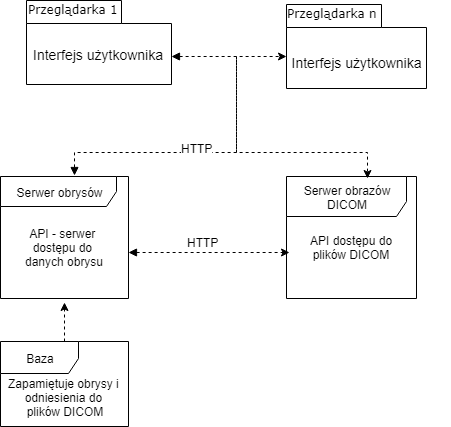
\includegraphics[width=0.7\textwidth]{architektura}
	\caption{Diagram UML przedstawiający architekturę autorskiego systemu}
    	\label{fig:architektura}
\end{figure}

\subsection {Interfejs użytkownika}

Kluczowym elementem stworzonego systemu jest interfejs użytkownika napisany w
języku skryptowym JavaScript przy użyciu biblioteki ReactJS. Udostępnia ona
interfejs nawigujący po~zapisanych w~serwerze Orthanc plikach DICOM. Ponadto dla
wyświetlonego obrazu udostępnia szczegóły dotyczące akwizycji obrazu, rodzaju badania i~danych pacjenta.
Umożliwia także wykonanie obrysu manualnego zrealizowanego przy użyciu biblioteki
\textit{react-canvas-draw} \cite{React canvas draw}. W~aplikacji zawarto również autorski interfejs do~wyboru punktów
do algorytmu półautomatycznego, wykonany z~użyciem elementu \textit{canvas} \cite{Canvas}.
Podgląd zapisanych w~systemie obrysów wraz z~wyliczonymi dla nich statystykami
jest możliwy z~poziomu tworzenia obrysów oraz w~osobnej zakładce, gdzie udostępniono
widok, w~którym użytkownik może oglądać jednocześnie wybrane przez siebie obrysy
z listy obrysów na~jednym obrazie.

\subsection {Serwer obrazów Orthanc}

Wyświetlane w~interfejsie użytkownika obrazy DICOM oraz związane z~nimi informacje
przechowywane są przez serwer DICOM. Dostęp do~zapisanych na~serwerze danych jest
możliwy poprzez udostępniane przez serwer API. Interfejs użytkownika wykorzystuje
API poprzez protokół HTTP.

API serwera udostępnia informacje o obrazach, takie jak: dane pacjenta,
rodzaj badania oraz serii. Wykorzystano je~w~interfejsie użytkownika do~nawigacji pomiędzy
obrazami. Dodatkowo dla każdego obrazu serwer udostępnia dane obrazowe, umożliwiając
wyświetlenie obrazu w~interfejsie użytkownika. Ponadto API udostępnia wszystkie
tagi obrazu DICOM, co~umożliwia wyświetlanie w interfejsie użytkownika informacji
w nich zawartych.

\subsection {Serwer obrysów i~statystyk}
Kolejny kluczowy element stworzonego systemu to~serwer obrysów i~obliczeń. Udostępnia
on API z~obrysami, które zostało wykorzystane przez interfejs użytkownika. API zostało
stworzone przy pomocy ASP.NET Core 2.2 \cite{ASPNET} i wykorzystaniu frameworka
.NET Core 2.2 \cite{Charakterystyka dotnet}. API oferuje cztery podstawowe operacje CRUD
- utwórz, odczytaj, aktualizuj i~usuń. W~celu pobrania obrazów medycznych serwer z~API
łączy się do~bazy danych Orthanc. Informacje o~obrysach, takie jak: ID~obrysu, tag,
ID obrazu medycznego i~typ obrysu (półautomatyczny lub manualny) są przechowywane
w bazie danych Microsoft SQL Server. Pozostałe informacje takie jak: lista pikseli
należących do~obrysu, lista punktów w~przypadku obrysu półautomatycznego i~statystyki
są przechowywane w~plikach CSV. Te~pliki są zapisywane w~katalogu roboczym obok
miejsca przechowywania plików źródłowych dla API.

Poza serwerem Orthanc interfejs korzysta także z~serwera przechowującego obrysy,
a także wykonującego obliczenia związane z~generowaniem obrysów. Serwer ten jest
dostępny dla interfejsu użytkownika poprzez API dostępne przez protokół HTTP.
Pozwala ono na~pobieranie zapisanych obrysów, zapisywanie obrysów manualnych
i~generowanie podglądu i~zapis obrysu półautomatycznego.

\subsection {Baza danych}

W celu zapisania danych związanych z~obrysami wykorzystana została baza SQL~Lite.
Baza składa się z~jednej tabeli, w~której przechowywane są: identyfikator obrazu DICOM,
identyfikator obrysu, nazwa obrysu oraz informacja o tym, czy obraz został wygenerowany
manualnie czy półautomatycznie. Punkty, z których składa się obrys i~statystytki
z~nim związane zapisywane są~w~oddzielnych
plikach tekstowych o nazwie identycznej z identyfikatorem obrysu.

\section {Moduł obrysów manualnych}

Moduł obrysów manualnych służy do~samodzielnego wykonywania obrysów przy użyciu myszy albo tabletu
graficznego. Obrysy wykonywane są poprzez przesuwanie przez użytkownika kursora
z~wciśniętym lewym przyciskiem myszy po~ekranie. Daje to użytkownikowi całkowitą
kontrolę nad kształtem wykonywanego przez niego obrysu. Dzięki temu modułowi
użytkownik może otrzymać obrys w sytuacji,
gdy moduł obrysów półautomatycznych nie daje użytkownikowi satysfakcjonujących rezultatów.

Obrysy manualne generowane przez użytkowników zapisywane są przez serwer obrysów
i~obliczeń w~postaci plików CSV na~dysku serwera. Na obrys składa się lista
pozycji punktów na obrazie, przez które użytkownik przesuwał kursor, a~także kolor obrysu.
W~momencie zapisu obrysu do pliku obliczane są
również statystyki dotyczące obrysowanej części obrazu, takie jak: długość obrysu,
pole obrysu, środek ciężkości obrysu, histogram regionu zainteresowania zawartego w obrysie oraz
liczba pikseli wewnątrz obrysu.

W związku z~tym, że obrazy wyświetlane w~interfejsie są w~innej rozdzielczości
niż rzeczywisty rozmiar obrazu (spowodowane jest to potrzebą zapewnienia, że obrys
będzie wyświetlany na ekranie w całości, jak również faktem, że obrazy o małej rozdzielczości
będą dostatecznie czytelne dla użytkownika), to obrysy przed zapisaniem zostają przeskalowane do
faktycznych wymiarów obrazu poprzez przemnożenie współrzędnych zaznaczonych przez
użytkownika punktów przez odwrotność współczynnika skalowania obrazu.
Natomiast w~przypadku obrazów o~małych rozdzielczościach może
spowodować to~utratę dokładności obrysu, a~w~przypadku obrysów bardzo małych
obszarów zdegradowanie obrysu do~jednego piksela, co~zostało przedstawione na Rysunku
\ref{fig:manual-0px}. Tego typu straty mogą wpływać
na poprawność obliczanych statystyk, jak również błędne wyświetlanie zapisanych
obrysów w~interfejsie użytkownika.

\begin{figure}[h]
	\center
	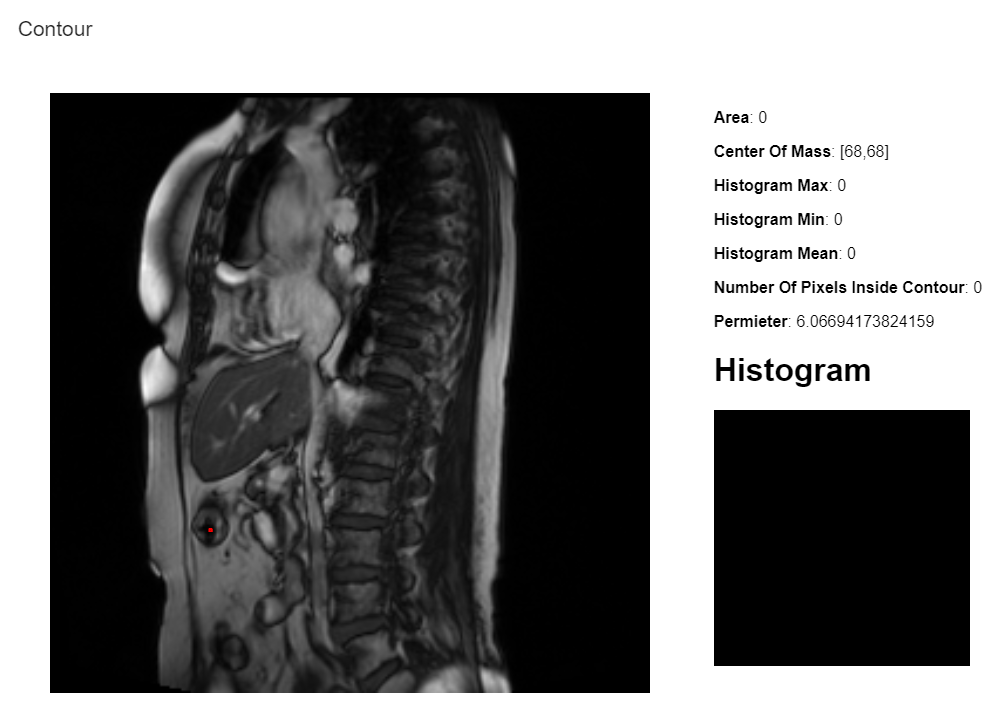
\includegraphics[width=0.9\textwidth]{manualny-0px}
	\caption{Przykład obrysu bez pikseli wewnątrz ze względu na niską rozdzielczość obrazu}
    	\label{fig:manual-0px}
\end{figure}

\section {Moduł obrysów półautomatycznych}

Moduł obrysów półautomatycznych pozwala użytkownikowi na~generowanie
obrysów poprzez wybieranie punktów na~obrazie DICOM. Wybrane punkty łączone są
ze sobą na~podstawie autorskiego algorytmu opisanego w~tym podrozdziale.

\subsection {Algorytmy generowania półautomatycznego obrysu}

Często na~obrazach medycznych różnice w~charakterystyce poziomów szarości pikseli
reprezentujących interesujące nas obiekty są~nieznaczne. Pliki zawierające te~obrazy medyczne często nie posiadają
dodatkowych informacji o~położeniu tych obiektów, ani czym się wyróżniają i~co~przedstawiają.
Problem opracowania uniwersalnego algorytmu wykrywania krawędzi na~obrazach medycznych
jest problemem trudnym. Takie algorytmy muszą spełniać szereg wymagań,
które stwierdzają poprawność danego algorytmu, jak również operatora morfologicznego.
Dla wielu takich algorytmów można znaleźć odpowiednie przykłady,
dla których krawędzie nie zostaną wyznaczone poprawnie. Według J.~Cytowskiego \cite{Cyfrowe przetwarzanie
obrazów medycznych} dobry detektor krawędzi powinien mieć niskie prawdopodobieństwo
zaznaczenia punktów nienależących do~krawędzi, oraz niskie prawdopodobieństwo
niezaznaczenia punktów należących do~krawędzi. Ponadto zaznaczone punkty krawędzi
przez taki detektor powinny być możliwie blisko jej osi. Ostatnim warunkiem, który powinien
spełniać taki detektor jest udzielanie minimalnej odpowiedzi, co~można rozumieć jako zwracanie
tylko jednej krawędzi dla jednej prawdziwej krawędzi, zaś szum nie powinien powodować
fałszywych detekcji. Nie można tego powiedzieć o~detektorze, który podzieli jedną krawędź
na~dwie lub zwróci dwie położone bardzo blisko siebie równoległe zamiast jednej.

Detektory krawędzi oparte na~gradiencie, w~tym operator Canny'ego są~często używane
zarówno w~przetwarzaniu obrazów medycznych, jak i~innych bardziej ogólnych zastosowaniach
w~innych dziedzinach nauki. Stosuje się je~do obrazów, które mają duże różnice w~luminancji i~nie
są~zaszumione. W~przypadku obrazów medycznych często możemy mówić właśnie o~takich obrazach.
Główne zalety detektorów krawędzi opartych na~krawędzi
wymienione w~\cite{Cyfrowe przetwarzanie obrazów medycznych}, to:
\begin{itemize}[noitemsep]
\item dobre wyniki dla obrazów o~dobrej jakości i~bez szumów,
\item odpowiednia wydajność --- złożoność algorytmów powinna być liniowa względem liczby przetwarzanych pikseli,
\item brak zastosowania metod o~dużej złożoności obliczeniowej, skomplikowanych metod sztucznej inteligencji.
\end{itemize}

Natomiast do~głównych wad tych algorytmów można zaliczyć:
\begin{itemize}[noitemsep]
\item potrzebę określenia rozmiaru maski i~wartości progowej, gdyż rozmiar maski
znacząco wpływa na~rozmieszczenie pozycji, w~których gradient osiąga wartości
maksymalne lub~przecina zera,
\item pomijanie narożników, które spowodowane jest faktem, że~wartość 1D~gradientu
w narożnikach jest zazwyczaj zbyt mała, aby wykrywać krawędzie wokół nich,
\item znajdowanie schodkowych krawędzi, które są wykrywane tylko przez operator pierwszej pochodnej,
\item dużą wrażliwość na~szum,
\item na~podstawie obserwacji działania algorytmu --- rozmyte krawędzie często
nie są wykrywane przez małe różnice w~wartościach kolejnych sąsiadujących pikseli.
\end{itemize}

Poniżej po krótce przedstawiono ogólny opis działania detektorów krawędzi opartych na~gradiencie,
na~przykładzie operatora Canny'ego \cite{Canny}. Wymyślony przez Canne'go operator
składa się z~trzech~zasadniczych kroków:
\begin{enumerate}%[noitemsep]
\item Określenie wartości i~kąta gradientu \\
W celu wyznaczenia wartości oraz kąta gradientu należy wykorzystać operator gradientu,
który będzie estymatorem gradientu w funkcji dyskretnej, jaką jest obraz.
Stosuje się takie operatory jak Krzyż Robertsa, Prewitta czy też operator Sobela.
Wykorzystując jeden z~takich operatorów,~uzyskano dla każdego piksela wielkość oraz
kierunek gradientu, co służy do~dalszych obliczeń,
\item Wykrycie miejsc występowania krawędzi \\
W tym celu został wykorzystany algorytm usuwania niemaksymalnych pikseli
(ang. \textit{non-max suppression}). Polega on~na~wyborze
takich pikseli, które mają największą wartość gradientu na~linii o~kierunku
zgodnym z~kątem danego gradientu. Możliwe są cztery kierunki: pionowy, poziomy oraz
dwa diagonalne. Jeśli dany piksel miał większą wartość gradientu od~dwóch swoich
sąsiadów, to~zaznaczono go~jako potencjalny punkt tworzący krawędzie. W~ten sposób
otrzymano obraz z~potencjalnymi krawędziami,
\item Wyznaczanie krawędzi progowaniem histerezy \\
Po poprzednim kroku na~obrazie nadal znajdują się nieistotne krawędzie. W~tym celu
Canny wprowadził ideę progowania histerezy. Metoda ta~wymaga dwóch wartości progowych
$T_1, T_2$ takich, że $T_1 < T_2$. Jeżeli wartość gradientu w~danym pikselu jest
większa od~$T_2$, to~zaznaczono ten punkt jako krawędź. Jeśli tak się stało, to
zaczęto proces śledzenia krawędzi --- dla każdego sąsiada, którego wartość gradientu
jest większa od~$T_1$ zaznaczono go~jako krawędź. Jest ona wykonywana rekurencyjnie
dla każdego zakwalifikowanego punktu.

Zamiast dokładnych wartości progowych można przekazać do~funkcji dwie wartości ---
$t_1, t_2$, które są procentem liczby pikseli, które będą niedopuszczone jako
krawędzie. Dla~$t_1~=~0.7, t_2 = 0.9$ dopuszczono tylko 10\% pikseli jako te,
które są większe od~$T_2$. Podając $t_1, t_2$ wyznaczono rozkład wartości
gradientu w~badanym obrazie, obliczono dystrybuantę $F(x)$ i~wybrano dla $T_1$
ten argument, dla którego $F(x) = t_1 * p$, gdzie $p$ to~liczba pikseli i~analogicznie
dla $T_2$. W~ten sposób wyznaczono progi do~histerezy.

\end{enumerate}

W celu obliczenia wartości oraz kąta gradientu stosuje się operator gradientu.
Istnieją różne rozwiązania obliczenia gradientu, a~najczęściej wykorzystuje się
do~tego operator Sobela, Prewitta lub Krzyż Robertsa. Krzyż Robertsa ma~najmniejszą złożoność,
lecz także wykazuje największą wrażliwość na~szumy. Operator Sobela i~Prewitta
mają podobną złożoność obliczeniową, ale~operator Sobela lepiej wygładza
krawędzie niż operator Prewitta. Z~wyżej wymienionych powodów w~autorskim rozwiązaniu
zdecydowano się użyć operatora Sobela w~celu obliczenia wartości oraz~kąta gradientu.
Założenia i~sposób działania tego operatora zostały przedstawione poniżej.

Operator Sobela \cite{Sobel} to~metoda wyznaczania gradientu, a~więc zarazem
krawędzi w~kierunku poziomym, jak i~w~pionowym. Dla każdego piksela
przeprowadzono operację morfologiczną z~następującymi maskami:

\begin{table}[h!]
\centering
\setlength{\tabcolsep}{40pt}
\begin{tabular} { c c }
  Maska rzędów & Maska kolumn \\
$
\begin{matrix*}[r]
-1 & -2 & -1 \\
0 & 0~& 0~\\
1 & 2~& 1
\end{matrix*}$
&
$\begin{matrix}
-1 & 0~& 1~\\
-2 & 0~& 2~\\
-1 & 0~& 1
\end{matrix}$
\end{tabular}
\end{table}

Po wykonaniu tych operacji otrzymano wartości $s_1$ i~$s_2$ odpowiednio dla maski
rzędów i~kolumn. Na~podstawie tych danych otrzymano następujące informacje o~gradiencie:
\begin{table}[h!]
\centering
\setlength{\tabcolsep}{30pt}
\begin{tabular} { c c }
  Wielkość gradientu & Kierunek krawędzi \\
$\sqrt{s_1^2 + s_2^2}$ & $tg^{-1} \Bigg[ {\cfrac{s_1}{s_2}} \Bigg]$
\end{tabular}
\end{table}

Podsumowując, w~dzisiejszych czasach w~celu zachowania niskiej złożoności obliczeniowej stosuje się
detektory krawędzi oparte na~gradiencie. Jednym z~takich detektorów jest operator Canny'ego. W~celu obliczenia
gradientu w~autorskim rozwiązaniu zastosowano operator Sobela, a~następnie aby wyznaczyć
położenia krawędzi zastosowano operator Canny'ego.

\subsection {Opracowany algorytm obrysów półautomatycznych}

Opracowany algorytm służy do~półautomatycznego tworzenia obrysów na~podstawie wybranych punktów,
które są interpolowane przez algorytm bazujący na~operatorze Canny'ego, operatorze
Sobela i~algorytmie A* (algorytm A* to~heurestyczny algorytm znajdowania najkrótszych ścieżek w~grafie).
Powyższe rozwiązania pozwalają na~uzyskanie satysfakcjonujących efektów na~przetwarzanych
przez narzędzie obrazach medycznych.
% screen z~aplikacji i~schemat

Danymi wejściowymi dla tego algorytmu obrysów półautomatycznych są:
\begin{itemize}[noitemsep]
\item {identyfikator obrazu medycznego, na~którym jest wykonywany obrys,}
\item {lista punktów wybranych przez użytkownika; punkty te~są~wcześniej
przeskalowywane ze~współrzędnych w~internetowej aplikacji webowej
na współrzędne odpowiadające rozdzielczości oryginalnego obrazu.}
\end{itemize}


Zaproponowany algorytm można podzielić na~kilka etapów:

\begin{itemize}[noitemsep]
\item {wygenerowanie bitmapy,}
\item {wykrycie krawędzi na~bitmapie,}
\item {stworzenie grafu z~bitmapy,}
\item {zapewnienie spójności grafu,}
\item {wyszukanie najkrótszych ścieżek w~grafie.}
\end{itemize}

Poniżej zostaną przedstawione dokładne rozwiązania dla każdego z~tych kroków.

\subsection {Wygenerowanie bitmapy}

W pierwszym etapie jest pobierany obraz medyczny o~danym wcześniej
identyfikatorze z~serwera Orthanc. Bitmapa tworzona jest na~podstawie obrazu DICOM poprzez
zapisanie w~odpowiednich komórkach wartości kolorów z~oryginalnego obrazu.
Stanowi ona podstawę do~dalszej pracy algorytmu.

\subsection {Wykrycie krawędzi na~bitmapie}

W pracy został użyty operator Canny'ego, ze~względu na~możliwość dostosowania
go~do~bardzo różnorodnych zagadnień detekcji obiektów w~obrazach medycznych.
Potwierdza to~porównanie operatorów wykrywania krawędzi zobrazowane przez
J.~Cytowskiego~\cite{Cyfrowe przetwarzanie obrazów medycznych}, operator Canny'ego
najlepiej wykrywał główne narządy, takie jak wątroba czy też trzustka, w~porównaniu
do~innych analizowanych narzędzi, takich jak operator Laplace'a czy też operatora \textit{zero-crossing}.

Stosując operator Canny'ego otrzymano macierz, gdzie każde pole w~macierzy odpowiada pikselowi
w wejściowej bitmapie --- obrazie medycznym. Jeśli w~komórce macierzy znajduje
się 1, to~w~tym miejscu na~bitmapie znajduje się krawędź, w~przeciwnym przypadku
0. W~ten sposób algorytm wykrył wszystkie znaczące krawędzie na~bitmapie. Kolejnym
krokiem przetwarzania było stworzenie grafu na~podstawie wyżej wymienionej macierzy.

Przykład działania operatora Canny'ego przedstawiono na~Rysunkach od \ref{fig:123} do \ref{fig:127}.
Obraz wyjściowy do dalszych działań został przedstawiony na Rysunku \ref{fig:123}.

%\begin{figure}[h!]
%	\center
%	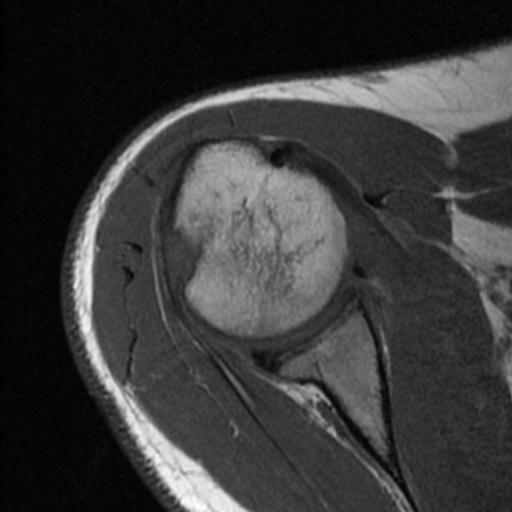
\includegraphics[width=0.45\textwidth]{123}
%	\caption{Oryginalny obraz, który przedstawia badanie rezonansem magnetycznym stawu ramiennego}
%	\label{fig:123}
%\end{figure}

\begin{figure}[p!]
	\center
	\minipage{0.48\textwidth}
		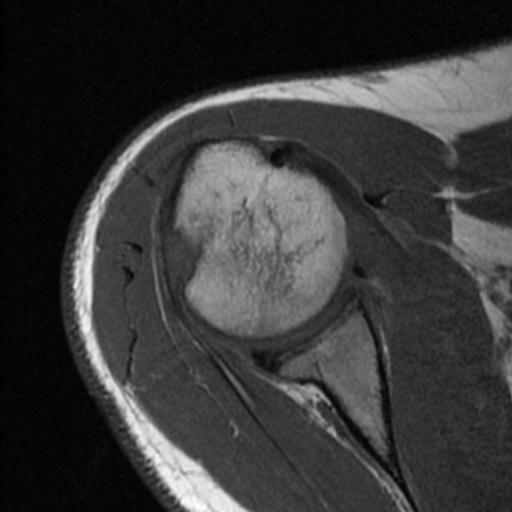
\includegraphics[width=\linewidth]{123}
		\caption{Oryginalny obraz, który przedstawia badanie rezonansem magnetycznym
		stawu ramiennego}%, jest on~obrazem wyjściowym do~dalszych rozważań}
		\label{fig:123}
	\endminipage
	\\
	\minipage{0.48\textwidth}
		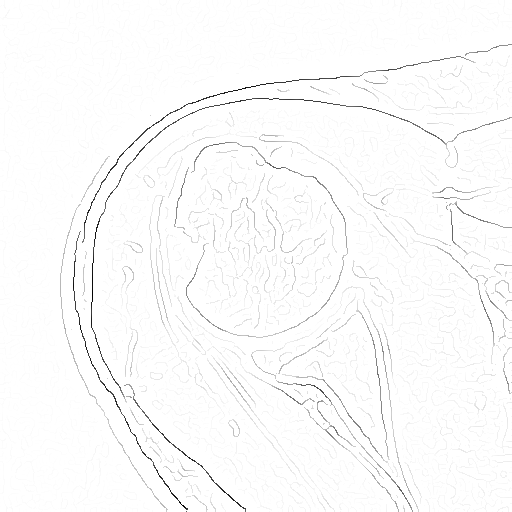
\includegraphics[width=\linewidth]{126}
		\caption{Obraz po~zastosowaniu algorytmu usuwania
	niemaksymalnych krawędzi nadal zawierający nieistotne krawędzie, które należy
	w~kolejnym kroku usunąć}
		\label{fig:126}
	\endminipage\hfill
	\minipage{0.48\textwidth}
		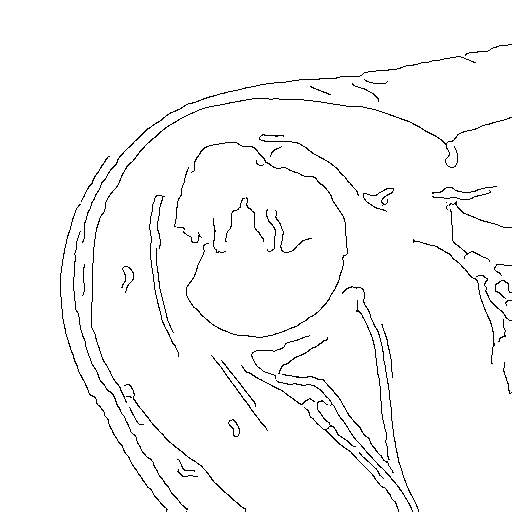
\includegraphics[width=\linewidth]{127}
		\caption{Wynikowa macierz po~zastosowaniu
	operatora Canny'ego, gdzie kolorem białym są
	reprezentowane wartości odpowiadające 0, a~kolor czarny odpowiada 1}
		\label{fig:127}
	\endminipage\hfill
\end{figure}

Po dwóch pierwszych krokach operatora Canny'ego, czyli wyznaczeniu gradientu i~zastosowaniu algorytmu
usuwania niemaksymalnych krawędzi uzyskano obraz z~potencjalnymi krawędziami. Został on~przedstawiony
na Rysunku \ref{fig:126}.

W ostatnim kroku była przeprowadzana histereza. Wynikiem jej działania jest macierz z~informacjami
gdzie znajduje się krawędź. Na~Rysunku \ref{fig:126} wartościom 1~w~macierzy odpowiada kolor czarny,
a~wartościom 0~odpowiada kolor biały.

\subsection {Stworzenie grafu z~bitmapy}

Kolejnym etapem było stworzenie grafu z~bitmapy. Na~tym etapie danymi wejściowymi były:
\begin{itemize}[noitemsep]
\item macierz z~wartościami logicznymi prawda/fałsz określającymi, czy znajduje się w~danym
punkcie krawędź,
\item punkty wybrane przez użytkownika aplikacji.
\end{itemize}

%Jaki tutaj -? - czy --?
Przed rozpoczęciem działania algorytmu należy zapewnić łączność 4-krotną
(ang. \textit{pixel 4-connectivity}) \cite{Pixel connectivity}, zwaną także
sąsiedztwem von Neumanna. Przy łączności 4-krotnej sprawdza się tylko sąsiadów
w poziomie lub pionie zgodnie ze~schematem na~Rysunku \ref{fig:4pixel}.

%Opisać te~rysunki i~wywalić stąd - nie muszą być dokładnie w~tym miejscu.
\begin{figure}[h!]
\begin{center}
	\minipage{0.48\textwidth}
	\begin{center}
		\begin{tikzpicture}
			\draw[step=1cm,gray,very thin] grid (3,3);
			\fill[fill=black!60!white, draw=black] (1,1) rectangle (2,2);
			\fill[fill=gray!60!white, draw=black] (1,0) rectangle (2,1);
			\fill[fill=gray!60!white, draw=black] (0,1) rectangle (1,2);
			\fill[fill=gray!60!white, draw=black] (2,1) rectangle (3,2);
			\fill[fill=gray!60!white, draw=black] (1,2) rectangle (2,3);
		\end{tikzpicture}
		\caption{Ilustracja łączności 4-krotnej}
		\label{fig:4pixel}
	\end{center}
	\endminipage\hfill
	\minipage{0.48\textwidth}
	\begin{center}
		\begin{tikzpicture}
			\draw[step=1cm,gray,very thin] grid (3,3);
			\fill[fill=black!60!white, draw=black] (1,1) rectangle (2,2);
			\fill[fill=gray!60!white, draw=black] (1,0) rectangle (2,1);
			\fill[fill=gray!60!white, draw=black] (0,1) rectangle (1,2);
			\fill[fill=gray!60!white, draw=black] (2,1) rectangle (3,2);
			\fill[fill=gray!60!white, draw=black] (1,2) rectangle (2,3);
			\fill[fill=gray!60!white, draw=black] (0,0) rectangle (1,1);
			\fill[fill=gray!60!white, draw=black] (2,2) rectangle (3,3);
			\fill[fill=gray!60!white, draw=black] (0,2) rectangle (1,3);
			\fill[fill=gray!60!white, draw=black] (2,0) rectangle (3,1);
		\end{tikzpicture}
		\caption{Ilustracja łączności 8-krotnej}
		\label{fig:8pixel}
	\end{center}
	\endminipage\hfill
\end{center}
\end{figure}

Dla łączności 8-krotnej sprawdza się wszystkich możliwych sąsiadów, także po
przekątnej. Jest ona zwana także sąsiedztwem Moore'a lub otoczeniem Moore'a \cite{Moore}.
Została ona przedstawiona na~Rysunku \ref{fig:8pixel}.

%\begin{figure}[h!]
%\begin{center}
%\begin{tikzpicture}
%\draw[step=1cm,gray,very thin] grid (3,3);
%\fill[fill=black!60!white, draw=black] (1,1) rectangle (2,2);
%\fill[fill=gray!60!white, draw=black] (1,0) rectangle (2,1);
%\fill[fill=gray!60!white, draw=black] (0,1) rectangle (1,2);
%\fill[fill=gray!60!white, draw=black] (2,1) rectangle (3,2);
%\fill[fill=gray!60!white, draw=black] (1,2) rectangle (2,3);
%\fill[fill=gray!60!white, draw=black] (0,0) rectangle (1,1);
%\fill[fill=gray!60!white, draw=black] (2,2) rectangle (3,3);
%\fill[fill=gray!60!white, draw=black] (0,2) rectangle (1,3);
%\fill[fill=gray!60!white, draw=black] (2,0) rectangle (3,1);
%\end{tikzpicture}
%\end{center}
%\caption{Ilustracja łączności 8-krotnej}
%\label{fig:8pixel}
%\end{figure}

%Bibliografia do~tego?
W przypadku zastosowania łączności 8-krotnej przy wyznaczaniu długości krawędzi
trzeba zastosować metrykę Czebyszewa, która jest specjalnym przypadkiem
odległości Minkowskiego. Przy zastosowaniu łączności 4-krotnej długość krawędzi
jest obliczana zgodnie z~metryką miejską, zwaną też metryką Manhattan.

Metryka Manhattan w~kontekście dalszego przetwarzania w~celu wyszukiwania
najkrótszych ścieżek w~grafie jest bardziej adekwatna, ponieważ jest intuicyjna
w wyznaczaniu odległości na~obrazie płaskim w~porównaniu do~metryki Czebyszewa.
W tym przypadku najlepsza byłaby tutaj metryka Euklidesa, lecz mamy do~czynienia
nie z~kolejnymi punktami oddalonymi od~siebie, a~z~sąsiadującymi pikselami.
Ponadto w~tym algorytmie istotne jest szybkie szacowanie odległości, czy też
długości danej krawędzi.

Wykrywanie wierzchołków przy łączności 4-krotnej jest prostsze. Wystarczy zliczyć
liczbę sąsiadów. Poniżej zakładamy, że piksel jest oznaczony jako krawędź w~macierzy
wejściowej. W~zależności od~liczby sąsiadów mamy następujące przypadki:
\begin{itemize}[noitemsep]
\item 0~--- wierzchołek izolowany,
\item 1~--- punkty końcowe (ang. \textit{endpixels}),
\item 2~--- punkty łączące (ang. \textit{linkpixels}), czyli fragmenty krawędzi,
\item 3--4 --- punkty węzłowe (ang. \textit{vertices}), czyli punkty, od~których odchodzą
co najmniej trzy krawędzie.
\end{itemize}

W przypadku łączności 8-krotnej do~detekcji wierzchołków należałoby stosować
przekształcenia Hit-or-Miss z~elementami strukturalnymi. Elementy strukturalne
do wykrywania odpowiednich punktów są następujące:

\begin{itemize}%[noitemsep]
\item wierzchołek izolowany: \\
$
\begin{bmatrix}
0 & 0~& 0~\\
0 & 1~& 0~\\
0 & 0~& 0
\end{bmatrix}
$,
\item punkty końcowe (ang. \textit{endpixels}): \\
$
\begin{bmatrix}
0 & 0~& 0~\\
0 & 1~& 0~\\
z & z~& z
\end{bmatrix}
$,
\item punkty łączące (ang. \textit{linkpixels}) --- fragmenty krawędzi, posiadają
dokładnie dwa punkty sąsiadujące, nie używane są przekształcenia Hit-or-Miss, a~tylko są liczone punkty sąsiadujące,
\item punkty węzłowe (ang. \textit{vertices}), czyli punkty, od~których odchodzą co~najmniej trzy krawędzie: \\
$
\begin{bmatrix}
z & 1~& z~\\
z & 1~& z~\\
z & z~& 1
\end{bmatrix}
$ lub $
\begin{bmatrix}
1 & z~& z~\\
z & 1~& z~\\
1 & z~& 1
\end{bmatrix}
$.
\end{itemize}

Warto zauważyć, że te~elementy strukturalne należy obracać o~90\textdegree, 180\textdegree~i~270\textdegree.
Za każdym razem trzeba by~wielokrotnie sprawdzać te~same piksele. Ponadto należy
stosować spójność 8-krotną, a~nie 4~krotną.

Kolejnym problemem jest fakt, że przy spójności 8-krotnej przekształcenie
Hit-or-Miss może w~najbliższym otoczeniu punktu krzyżowania się krawędzi oznaczyć
kilka otaczających punktów, jako punkty węzłowe. Jest to~złe rozwiązanie, ponieważ
w ten sposób może nawet kilkukrotnie zwiększyć liczbę wierzchołków w~grafie, co
przełożyłoby się na~niską wydajność algorytmu.

Ostatnim problemem, który należałoby rozwiązać wybierając łączność 8-krotną
jest fakt, że macierz wejściową dla tego etapu algorytmu trzeba by~poddać procesowi
szkieletyzacji. Najlepiej byłoby w~tym celu skorzystać z~algorytmu KMM \cite{KMM}
lub K3M \cite{K3M}. Te~algorytmy, w~optymistycznym przypadku, musiałyby co~najmniej
raz przeanalizować całą macierz z~wykrytymi krawędziami.

\bigskip

W pracy zdecydowano się na~metrykę 4-krotną ze~względu na~prostotę obliczeń,
która skróciła czas pracy algorytmu. Nie wymagało to~także dodatkowych
obliczeń związanych ze~szkieletyzacją (ang. \textit{thinning}). Przygotowano
i~zaimplementowano algorytm tworzący graf z~bitmapy, a~jego pseudokod znajduje
się w~Załączniku 1.

Utworzony w~ten sposób graf był grafem nieskierowanym z~wagami, gdzie wagi to
liczba pikseli, czy też liczba punktów należących do~krawędzi. Graf ten mógł nie być
spójny. Ponadto mógł nie zawierać wierzchołków, które pokrywały się z~punktami
wybranymi przez użytkownika.

Graf ten zazwyczaj był rzadki, ponieważ liczba jego krawędzi była rzędu liczby
jego wierzchołków.  Z~uwagi na~czasami bardzo dużą liczbę wierzchołków, nawet
do kilkudziesięciu tysięcy, próba implementacji przy pomocy macierzy sąsiedztwa
mogłaby spowodować zużycie całej możliwej pamięci operacyjnej. Dla 50~tysięcy
wierzchołków program musiałby zadeklarować macierz sąsiedztwa zawierającą 2,5
miliarda komórek. Z~tych powodów graf został zaimplementowany przy pomocy list sąsiedztwa.

W przyjętej implementacji każda krawędź zawierała dodatkowo informację o~tym, jakie
piksele należały do~danej krawędzi w~rzeczywistym obrazie.

\subsection {Zapewnienie spójności grafu}

W pierwszym kroku na~tym etapie przetwarzania grafu są dodawane punkty wybrane
przez użytkownika do~grafu.

Graf, który uzyskano w~poprzednim kroku może nie być spójny. Powoduje to~fakt,
że między punktami wybranymi przez użytkownika mogą nie istnieć ścieżki. W~celu
zapewnienia spójności grafu należy dodawać sztuczne krawędzie. Zostają one dodawane
z większymi wagami, niż wynikałoby to~w~rzeczywistości z~liczebności listy pikseli,
które reprezentują, ponieważ ma~to~na~celu używanie z~większym priorytetem prawdziwych
krawędzi, a~nie sztucznych. W~sytuacji gdy nie istnieje dobra ścieżka z~prawdziwych
krawędzi, zostaną użyte krawędzie sztuczne. Duże wagi dodatkowo będą zmuszały
algorytmy wyszukiwania najkrótszych ścieżek w~grafie do~minimalizowania długości
takich fragmentów zawierających sztuczne krawędzie.

Do znajdowania spójnych składowych grafu najczęściej używa się algorytmu
przeszukiwania grafu w~głąb (ang. \textit{Depth-first search}, w~skrócie DFS) lub
przeszukiwania grafu wszerz (ang. \textit{Breadth-first search}, w~skrócie BFS)
\cite{Algorytmy Sedgewick}. Użyto algorytmu przeszukiwania wszerz, opierając się
na przykładowej implementacji w~materiałach \cite{AiSD2}. Ponieważ zdecydowano się
na~przeszukiwanie wszerz, to wykorzystano \textit{Queue<T>}, a~zatem kolejkę. Dla tego zagadnienia
nie ma różnicy czy wybrano przeszukiwanie wszerz, czy też w~głąb. Złożoność
obliczeniowa tego algorytmu przeszukiwania to~$O(|E|)$.

Po wyznaczeniu spójnych składowych grafu dla każdej pary składowych znajdowano
taką parę wierzchołków, żeby odległość między nimi była minimalna. Jeśli odległość
była mniejsza niż maksymalna odległość między dwoma dowolnymi punktami zaznaczonymi
przez użytkownika, to~była dodawana sztuczna krawędź o~wadze 2,5 razy większej
niż odległość wynikająca z~metryki Manhattan pomiędzy tymi dwoma wierzchołkami.

Przykład zasady działania tej operacji przedstawia poniższy pseudokod:

\begin{verbatim}
foreach (Spójna składowa grafu s1)
{
    foreach (Spójna składowa grafu s2, różna od s1 i nie przetwarzana
      wcześniej jako s1)
    {
        Wybierz wierzchołek v1 z s1 i v2 z s2 takie, że odległość pomiędzy
          nimi jest najmniejsza ze wszystkich takich par
        Dodaj sztuczną krawędź pomiędzy v1 i v2
    }
}
\end{verbatim}


W ten sposób osiągnięto spójny graf, który zawiera punkty dodane przez użytkownika.

\subsection {Wyszukanie najkrótszych ścieżek w~grafie}

Na tym etapie została zapewniona spójność grafu. Z~całą pewnością istnieje ścieżka
pomiędzy punktami wybranymi przez użytkownika, te~punkty są osiągalne. Pozostało
wybrać najkrótszą ścieżkę łączącą kolejne punkty. Założono, że jest dana lista
punktów wybranych przez użytkownika i~zawiera ona kolejne punkty, tzn. algorytm
prowadzi ścieżkę od pierwszego punktu przez kolejne punkty wybrane przez użytkownika
aż~do~ostatniego takiego punktu. Następnie jest łączony ostatni punkt z~pierwszym.

Warto zaznaczyć, że wyszukiwano ścieżki o~minimalnej wadze, czy też o~minimalnym
koszcie. Z~uwagi na~fakt, że wagi w~grafie są ściśle związane z~odległościami to
używane jest sformułowanie szukania najkrótszych ścieżek. Wagi w~tym grafie są
nieujemne. Może w~nim istnieć kilka ścieżek z~jednego punktu do~drugiego o~tym
samym koszcie, więc algorytm kończy swoje działanie na~tym etapie, gdy znajdzie
jedną z~nich. W~tym grafie nie występują krawędzie wielokrotne i~graf nie zawiera
cykli własnych.

Do wyszukiwania najkrótszych ścieżek w~grafie, po~zgłębieniu literatury
\cite{Algorytmy Sedgewick} i~\cite{AiSD2} były rozważane do~użycia dwa~algorytmy.
Był to~algorytm Dijkstry i~algorytm A*. Do~algorytmu A* była rozważana heurystyka w~postaci
odległości miejskiej, Manhattan z~wierzchołka $v$ do~celu $t$, ozn. $h(v)$.

Zgodnie z~\cite{AiSD2} ,,Funkcja $h$ musi spełniać następujące warunki:

\begin{itemize}[noitemsep]
\item musi być oszacowaniem dolnym, czyli dla każdego wierzchołka $v$ $h(v) <=$ odległość $v$ od~celu $t$,
\item musi być monotoniczna, czyli dla dowolnej krawędzi $<u,v>$ $h(u) <= $waga$<u,v> + h(v)$.''
\end{itemize}

Heurystyka w~postaci metryki Manhattan spełnia te~wymagania. Z~tego powodu może
zostać wykorzystany algorytm A*. Porównując złożoności algorytmu A* i~Dijkstry w
\cite{AiSD2} możemy zauważyć, że algorytm A* w~pesymistycznym przypadku ma~taką
samą złożoność jak algorytm Djikstry, czyli $O(|E|*log(|V|))$ z~kolejką priorytetową
dla grafów rzadkich, a~$O(|V|^2)$ nie wykorzystując kolejki priorytetowej dla
grafów gęstych. W~praktyce dla grafów rzadkich nie ma~potrzeby rozważania znacznej
części wierzchołków, co~poprawia złożoność średnią. Wynosi ona wtedy $O(|E|)$.

Do implementacji wyszukiwania najkrótszych ścieżek w~grafie na~podstawie wyżej
wymienionych wniosków został wykorzystany algorytm A* z~heurystyką w~postaci
metryki Manhattan. Przykładowy pseudokod tego algorytmu można znaleźć w
\cite{AiSD2} i~jest on~następujący: %Także nie powinno tak tego się robić!

\begin{verbatim}
CLOSE = 0 // zbiór (z szybkim sprawdzeniem przynależności)
OPEN = {s} // kolejka priorytetowa
// priorytety - sumy odległości wierzchołków od źródła
// i oszacowań odległości tych wierzchołków od celu
odległość[s] = 0
while ( OPEN niepusty )
{
    u = wierzchołek należący do OPEN taki, że
        odległość[u] + oszacowanie[u,t] <=
        odległość[w] + oszacowanie[w,t]
        dla wszystkich w należących do OPEN
    usuń u z OPEN
    wstaw u do CLOSE
    if ( u == t ) break
    foreach ( wierzchołek w sąsiadujący z u taki, że w należący do CLOSE )
    {
        if ( w należy do OPEN )
        {
            odległość[w] = nieskończoność
            wstaw w do OPEN
        }
        if ( odległość[w] > odległość[u] + waga<u,w> )
        {
            odległość[w] = odległość[u] + waga<u,w>
            aktualizacja priorytetu wierzchołka w (w OPEN)
            poprzedni[w] = u
        }
    }
}
\end{verbatim}

W celu wykorzystania niskiej złożoności obliczeniowej algorytmu A*
należało zastosować dobre struktury danych do~tego algorytmu. Zbiór CLOSE
wymagał szybkiego sprawdzania przynależności. Po~przeanalizowaniu rekomendowanych
struktur danych \cite{Dotnet struktury} został użyty \textit{HashSet<T>}.

Zbiór OPEN oferował zastosowanie znacznie bardziej finezyjnych struktur danych.
Wymagano od~niego, aby był kolejką priorytetową, czyli aby był sortowany po
priorytetach będącymi sumą odległości wierzchołków od~źródła i~oszacowań odległości
tych wierzchołków od~celu. Warto zauważyć, że oprócz sortowania często były wstawiane
do niego wierzchołki, pobierane, usuwane i~modyfikowane wartości priorytetu.
Bardzo często była sprawdzana przynależność i~przeprowadzano
wyszukiwanie według klucza.

Porównanie czasów różnych operacji dla różnych klas słownikowych zaimplementowanych
w~technologii .NET można znaleźć w~\cite{C w pigulce}.
Najlepszym rozwiązaniem byłoby użycie \textit{SortedDictionary<K,V>},
która jest implementowana przez drzewo czerwono-czarne. Niestety jest
sortowana po~kluczu a~nie tak, jak jest potrzebne w~tym przypadku sortowanie
po wartości. Poszukiwano zatem struktury danych, która sortuje po~wartościach
i ma~łatwy dostęp przez klucz.

W zaproponowanym rozwiązaniu została zaimplementowana struktura danych opierająca się
na dwóch podstrukturach - zaimplementowanej kolejki priorytetowej poprzez listę
oraz słownik \textit{Dictionary<K,V>} z~technologii .NET, który opiera się na~tablicy
skrótów. Zaimplementowana lista miała następującą strukturę:

\begin{verbatim}
public class MySortedListElement
{
    public Vertex Key;
    public double Value;
    public MySortedListElement next;
    public MySortedListElement previous;
}
\end{verbatim}

Struktura ta~miała zaimplementowane sortowanie przez wstawianie, zatem modyfikacja
tylko jednego elementu wymagała w~pesymistycznym przypadku tylko $O(n)$ porównań.
Wstawianie nowego elementu ma~złożoność pesymistyczną $O(n)$, usuwanie $O(1)$.
Zbadanie przynależności po~kluczu to~$O(n)$ i~nie zaleca się tego robić.

Niezależnie od~tej struktury jest przechowywana druga struktura danych,
\textit{Dictionary<K,V>}, gdzie kluczami są wierzchołki, a~wartości to~referencje na
elementy tej listy. Zmienne odpowiedzialne za~przechowanie kolejki priorytetowej
OPEN zostały zadeklarowane w~sposób następujący:

\begin{verbatim}
Dictionary<Vertex, MySortedListElement> OpenDictionary =
   new Dictionary<Vertex, MySortedListElement>();
MySortedList OpenList = new MySortedList();
\end{verbatim}

W ten sposób w~połączeniu tych dwóch podstruktur otrzymano strukturę danych
o następujących własnościach:
\begin{itemize}[noitemsep]
\item dodawanie w~czasie $O(n)$,
\item wyszukiwanie po~kluczu w~czasie $O(1)$,
\item wybieranie najmniejszego elementu według wartości w~czasie $O(1)$,
\item usuwanie w~czasie $O(1)$
\item modyfikowanie jednego elementu w~czasie $O(n)$.
\end{itemize}

Algorytm A* jest uruchamiany dla każdego punktu wybranego przez użytkownika.
Wyszukuje on~najkrótszą ścieżkę do~kolejnego punktu wybranego przez użytkownika.
Po wszystkich obliczeniach obrys składa się z~poszczególnych ścieżek. Są one
konsolidowane i~zwracane jako lista pikseli na~podstawie danych z~krawędzi o
listach pikseli, z~których jest zbudowana krawędź. W~ten sposób jest wykrywany
obrys pomiędzy punktami zaznaczonymi przez użytkownika.

W sytuacji, gdy pomiędzy różnymi wierzchołkami nie istnieją prawdziwe krawędzie,
albo istnieją tylko w~wybranym fragmencie ścieżki łączącej te~dwa wierzchołki,
algorytm w~miarę możliwości będzie starał się używać prawdziwych krawędzi, dzięki
odpowiedniej wadze krawędzi sztucznych. Dzięki sztucznym krawędziom na~pewno
istnieje droga między kolejnymi punktami, zatem algorytm z~całą pewnością zwróci
poprawny wynik. Co~najwyżej będzie to~wielokąt z~punktami wybranymi przez użytkownika.

Algorytm dla sztucznych krawędzi generuje listę pikseli algorytmem Bresenhama
\cite{Bresenham}. Jest to~algorytm, który dodaje w~najbardziej optymalny sposób
krawędzie. W~celu zapewnienia łączności 4-krotnej jest przeprowadzana operacja
morfologiczna z~wykrywaniem 2~pikseli po~przekątnej z~maską 4-pikselową. Gdy takie
piksele zostaną wykryte, to~na~jednym z~rogów jest dodawany piksel w~celu
zapewnienia łączności 4-krotnej.

\subsection {Optymalizacja algorytmu obrysu półautomatycznego}

Większość obrazów medycznych ma~rozdzielczość rzędu kilkaset na~kilkaset pikseli,
a więc cały obraz zawiera kilkaset tysięcy pikseli. Zdarzają się też
pliki w~znacznie większej rozdzielczości, takimi są między innymi mammografia i
obrazy rentgenowskie rzędu kilku tysięcy na~kilka tysięcy pikseli.
Takie obrazy zawierają do~kilkudziesięciu milionów
pikseli. W~celu sprawnego przetwarzania tych obrazów potrzebne było przeprowadzenie optymalizacji
algorytmu, opisanej w dalszej części pracy.
\begin{enumerate}
\item Zmniejszenie rozmiaru obrazu roboczego \\
W pierwszym kroku zmniejszono rozmiar obrazu roboczego. Wyznaczono najmniejszy obszar
zainteresowania (ang. \textit{ROI --- Region of Interest}) w~kształcie
prostokąta, w~którym mieszczą się wszystkie punkty zaznaczone przez użytkownika.
Powiększono ten obszar o~marginesy w~taki sposób, by~wyjściowy prostokąt nadal
był w~środku, a~pole powiększonego było 4-krotnie większe. Innymi słowami,
dodano marginesy po~50\% szerokości/wysokości do~każdego wymiaru. Jeśli rozmiar
powiększonego prostokąta jest większy niż obrazu, to~nie jest zmieniany obraz roboczy.
Gdy użytkownik stworzył niewielki obrys, to~rozmiar obrazu jest także niewielki.
W sytuacji, gdy obrys zajmuje prawie cały obraz medyczny, to~nadal musi być
przetwarzany cały obraz.
\item Sięganie do~pamięci zamiast to~bitmapy \\
W celu przyśpieszenia działania operatora Sobela i~liczenia statystyk, zamiast
sięgać do~bitmapy metodą \textbf{.GetPixel()} na~platformie .NET, bitmapa została zapisana
do tablicy bajtów w~celu uzyskania bezpośredniego dostępu. Została wykorzystana do~tego
funkcja \textbf{.LockBits()}. Zysk na~tej operacji był kilkudziesięciokrotny. Na~późniejszych
etapach algorytmu pracowano na~macierzy, która nie była już bitmapą, więc operacje
te wykonywały się znacznie szybciej.
\item Dzielenie zbyt długich krawędzi \\
W sytuacji, gdy wczytane krawędzie do~grafu są bardzo długie, może zdarzyć się
taka sytuacja, że punkt zaznaczony przez użytkownika znajduje się bardzo blisko
krawędzi, ale daleko od~punktu początkowego lub końcowego krawędzi. W~tym celu
jest wprowadzony mechanizm dzielenia zbyt długich krawędzi na~kilka krótszych.
\item Problem z~liczbą punktów \\
Dla każdego punktu jest uruchamiany algorytm A*, zatem w~sposób liniowy od~ilości
punktów zależy liczba uruchomień algorytmu A*. Nie można wyznaczyć, czy w~złożoności
średniej całego algorytmu jest on zależny liniowo od~ilości punktów, czy
w sposób logarytmiczny, czy też w~sposób stały.
\end{enumerate}

\section {Moduł obliczeń statystyk}

System zapewnia liczenie statystyk dotyczących obrysu. Statystyki są identyczne
zarówno dla obrysów manualnych i~półautomatycznych, do~których należą:

\begin{itemize}[noitemsep]
\item histogram --- wykres pokazujący natężenie kolorów w~obrysowanym obszarze
(kolor, to~liczba w~zakresie $[0,255]$, gdzie 0~oznacza najciemniejszy piksel,
a 255 najjaśniejszy),
\begin{itemize}[noitemsep]
\item wartość maksymalna --- maksymalna wartość piksela wewnątrz obrysu,
\item wartość minimalna --- minimalna wartość piksela wewnątrz obrysu,
\item wartość średnia --- średnia arytmetyczna wartości pikseli wewnątrz obrysu,
\end{itemize}
\item środek ciężkości --- średnia arytmetyczna pozycji pikseli obrysu,
\item długość obrysu w~$mm$ --- obliczana na~podstawie położenia pikseli i~% doprecyzuj, bo~ja~nie wiem
wartości \textit{pixel spacing} odczytywanej z~tagu obrazu DICOM,
\item długość obrysu w~pikselach,
\item pole powierzchni w~$mm^2$,
\item liczba pikseli wewnątrz obrysu.
\end{itemize}

Przykładowe wygenerowane statystyki zostały przedstawione na~Rysunku \ref{fig:107b}.

\begin{figure}[h!]
	\center
	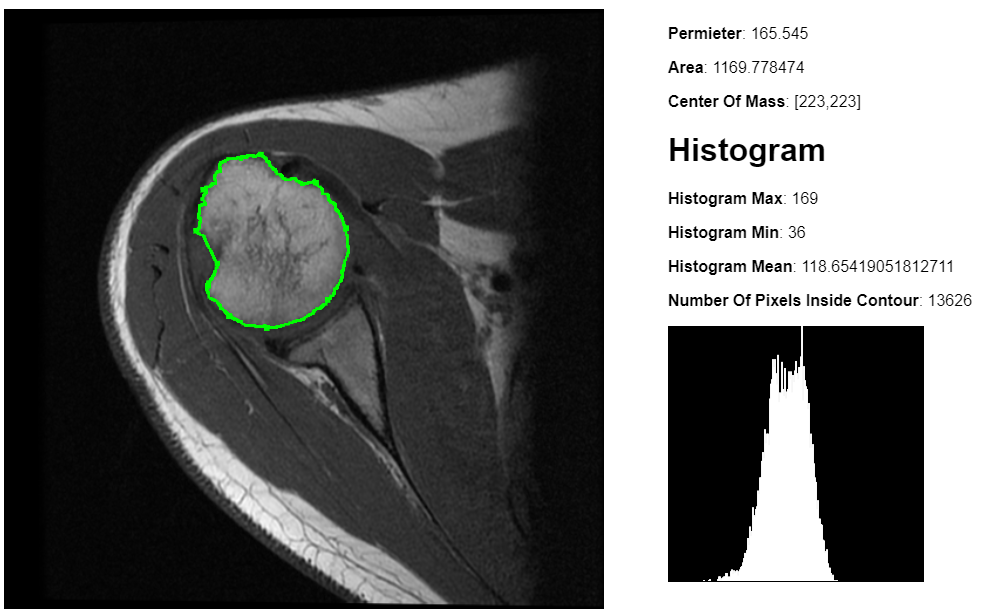
\includegraphics[width=0.8\textwidth]{107}
	\caption{Przykładowe wygenerowane statystyki}
    	\label{fig:107b}
\end{figure}

Do obliczenia histogramu jest wymagany punkt wewnętrzny obrysu. Środek ciężkości
obrysu nie zawsze musi znajdować się wewnątrz obrysu. W~przypadku zastosowania
algorytmu \textit{scan-linii} \cite{GK1} dla obrysu manualnego nie jest podana informacja o~logicznych
wartościach, gdzie jest krawędź, więc nie można wykryć np. krawędzi poziomych.
%Algorytm scan-linii lepiej nadaje się w~przypadku, gdy wypełniamy wielokąt,
%a nie obrys.
% pani dr~chciała to~inaczej

Z tego powodu wybrano algorytm \textit{Flood Fill} \cite{AiSD2}, czyli rozlewania się rekurencyjnego % cytacja
zliczonych pikseli od~punktu wewnętrznego. Właśnie z~tego powodu od~użytkownika
jest wymagane podanie dodatkowej informacji, jaką jest punkt wewnętrzny obrysu.
Założono, że użytkownik zaznaczy go~poprawnie. W~sytuacji, gdy zostanie podany
błędny punkt, to~ten algorytm policzy to, co~znajduje się poza regioniem zainteresowania (ROI),
a~nie to, co~znajduje się wewnątrz tego regionu.
%to~ten algorytm policzy to~co~znajduje się na~zewnątrz obrysu, a
%nie to~co~jest wewnątrz.

Długość obrysu w~pikselach jest obliczana na~podstawie liczebności listy pikseli należących do~obrysu.

\section {Moduł anonimizacji danych}

W celu umożliwienia anonimizacji danych pacjentów zawartych w~plikach DICOM skorzystano
z REST API serwera Orthanc. Umożliwia to wykonanie kopii badania wgranego do~serwera
z~nowymi danymi pacjenta. Po~wykonaniu kopii z~podanymi przez użytkownika danymi,
oryginalny obraz DICOM jest usuwany z~serwera obrazów Orthanc.

Danymi, które użytkownik może zmienić to~imię i~nazwisko pacjenta, data urodzenia pacjenta
i~płeć pacjenta. W miejsce wymienionych pól użytkownik może wpisać dowolne ciągi
znaków, w szczególności takie, które nie pozwolą na ustalenie tożsamości pacjenta.

\afterpage{\blankpage}

\chapter {Przeprowadzone eksperymenty}

%Zostały przeprowadzne eksperymenty na~autorskim narzędziu do~tworzenia obrysów.
Eksperymenty zostały przeprowadzone przy użyciu zaproponowanego narzędzia 
do~tworzenia obrysów pod kątem:
\begin{itemize}[noitemsep]
\item działania narzędzia z różnymi typami badań medycznych,
\item poprawności działania algorytmu obrysów półautomatycznych,
\item wydajności algorytmu obrysów półautomatycznych.
\end{itemize}
W podrozdziałach 4.1 - 4.4 przedstawiono wyniki tych eksperymentów.

Testy wykonano na~komputerze stacjonarnym o~następującej specyfikacji:
\begin{itemize}[noitemsep]
\item procesor Intel Core i5-7500 o~taktowaniu maksymalnym dla jednego rdzenia 3.8 Ghz;
\item pamięć RAM Corsair Vengeance DDR4 16GB 3000 Mhz ustawiona w~tryb 2140 Mhz o~opóźnieniach CL15;
\item płyta główna ASUS STRIX ROG Z270-I;
\item procesor jest chłodzony powietrzem przez Noctuę NH-L9i; procesor utrzymuje
temperaturę około 64~stopni Celsjusza przy temperaturze otoczenia około 21~stopni
Celsjusza; nie występuje throttling;
\item system operacyjny Windows 10.
\end{itemize}

\section {Zbiór testowy}

%Na zbiór plików testowych składają się prywatne badania autora i~jego najbliższej rodziny.
Zbiór danych testowych składał się z~20 badań, w~tym badania 
CT~(ang. \textit{computed tomography}~---~tomografia komputerowa), 
MRI~(ang. \textit{magnetic resonance imaging}~---~obrazowanie metodą rezonansu magnetycznego),
RTG, MMG. Badania te zostały wykonane na różnych urządzeniach, w~różnych placówkach medycznych.

Badania tomografią komputerową zazwyczaj składają się z~jednej serii. Ta seria zazwyczaj zawiera od~kilkudziesięciu
do~kilkuset kolejnych wartw, które są obrazami. Dla większości badań rozdzielczość takiego obrazu wynosiła 512 na 512 pikseli.

Badania rezonansem magnetycznym zazwyczaj składają się z~kilku do kilkunastu serii, gdzie każda seria zawierała kilkanaście warstw.
Rozdzielczość jednego obrazu składającego się na warstwę zazwyczaj wynosiła 512 na 512 pikseli.

Na badanie rentgenowskie składa się zazwyczaj jedna do kilku serii, gdzie każda zawiera jeden obraz. Rozdzielczość tego obrazu zazwyczaj wynosiła około 1952 na 1620 pikseli.

Mammogramy mają największą rozdzielczość. Jeden obraz składał się z 6000 na 3300 pikseli, co daje rozdzielczość prawie 20 megapikseli.

%Do testów zostały wykorzystane następujące badania:
%\begin{enumerate}[noitemsep]
%\item badanie rezonansem magnetycznym barku prawego Tomasza Świerczewskiego około
%8 tygodni po~zwichnięciu stawu ramiennego typu przedniego podkruczego --- Badanie 1,
%\item zdjęcie rentgenowskie barku prawego Tomasza Świerczewskiego w~momencie zwichnięcia stawu ramiennego --- Badanie 2,
%\item badanie tomografią komputerową kręgosłupa Wojciecha Świerczewskiego --- Badanie 3,
%\item badanie rezonansem magnetycznym kręgosłupa Wojciecha Świerczewskiego --- Badanie 4.
%\end{enumerate}

%W celu zaprezentowania działania algorytmu  wybrano jedno przykładowe badanie --- badanie MRI stawu ramiennego.

%Pliki te~były wykonane na~różnych urządzeniach, w~różnych szpitalach.

%Dodatkowo wykorzystano wyniki badań udostępnione Politechnice Warszawskiej do
%celów dydaktycznio badawczych. Zawierały one badania organów wewnętrznych, takich
%jak wątroba i~trzustka wykonane przy użyciu rezonansu magnetycznego oraz badanie mammograficzne.

\section {Analiza działania aplikacji}

%W autorskiej aplikacji otwierano kolejne badania. Rysunek \ref{fig:112} przedstawia
%jedną klatkę obrazu medycznego Badania 1, z~pewnej serii. Rysunek \ref{fig:113}
%przedstawia Badanie 2, natomiast Rysunek \ref{fig:114} przedstawia Badanie 3, a
%Rysunek \ref{fig:115} Badanie 4.

%Ten test wykazał, że aplikacja otwiera różne badania medyczne, od~rezonansu
%magnetycznego, przez tomografię komputerową po~zdjęcie rentgenowskie. Na~każdym
%z obrazów medycznych można wykonywać obrysy. Przykładowe obrysy ręczne i
%półautomatyczne znajdują się odpowiednio na~Rysunku \ref{fig:105} i~Rysunku
%\ref{fig:107}. Wyniki testów potwierdzają, że statystyki są obliczane poprawnie.

Przeprowadzano analizę działania autorskiego narzędzia do tworzenia obrysów.
W~pierwszym kroku przeprowadzono testy związane z~obsługą różnych typów badań.
Aplikacja obsługuje wszystkie przebadane typy badań, czyli CT, MRI, RTG, MMG.
Nie wykonano testów na innych typach badań takich jak cyfrowej angiografii subtrakcyjnej
i~wielu innych. Aplikacja powinna obsługiwać inne typy badań, ponieważ wspiera pliki DICOM.

W celu zaprezentowania funkcjonalności autorskiej aplikacji, na Rysunku \ref{fig:113} 
przedstawiono w~jaki sposób autorska aplikacja ukazuje 
użytkownikowi badanie RTG. 

\begin{figure}[h!]
	\center
	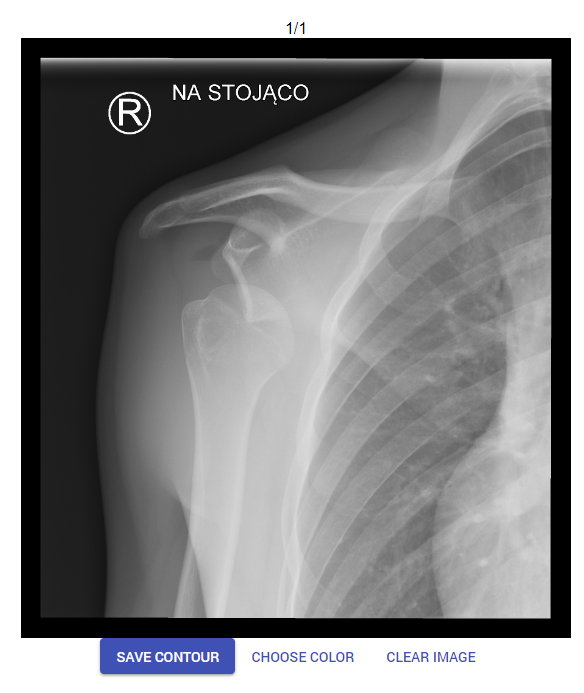
\includegraphics[width=0.6\textwidth]{113}
	\caption{Widok badania RTG barku}
    	\label{fig:113}
\end{figure}

Na Rysunku \ref{fig:140} przedstawiono inne badanie, MRI. Dodatkowo przedstawiono, 
że~aplikacja umożliwia zmianę wyświetlanej warstwy. Użytkownik ma~możliwość wybrania 
odpowiedniej warstwy z~listy, bądź wybranie następnej lub poprzedniej warstwy przez użycie
rolki myszy. Ta~funkcjonalność zadziała, gdy kursor myszy znajduje się nad obrazem.
Użytkownik ma także możliwość zmiany serii badania poprzez wybranie jej z~odpowiedniej listy.

\bigskip

\begin{figure}[h!]
\begin{center}
	\minipage{0.48\textwidth}
	\begin{center}
		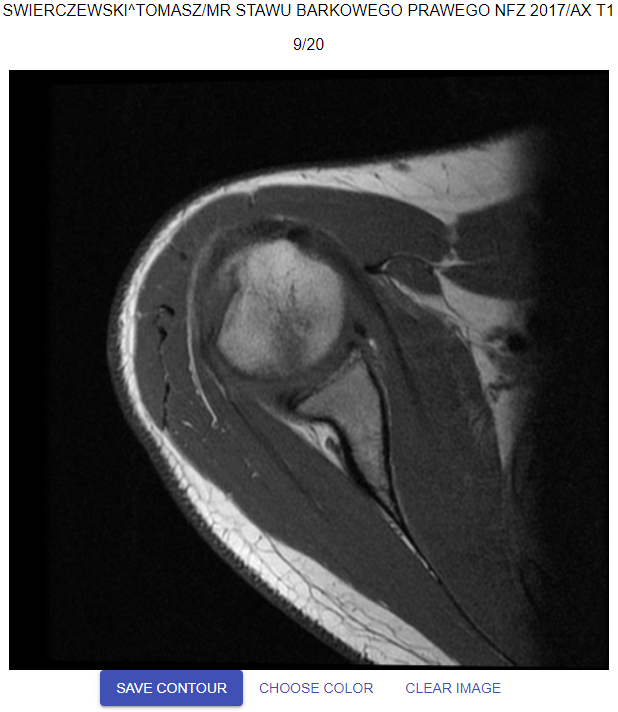
\includegraphics[width=1.0\textwidth]{141}
	\end{center}
	\endminipage\hfill
	\minipage{0.48\textwidth}
	\begin{center}
		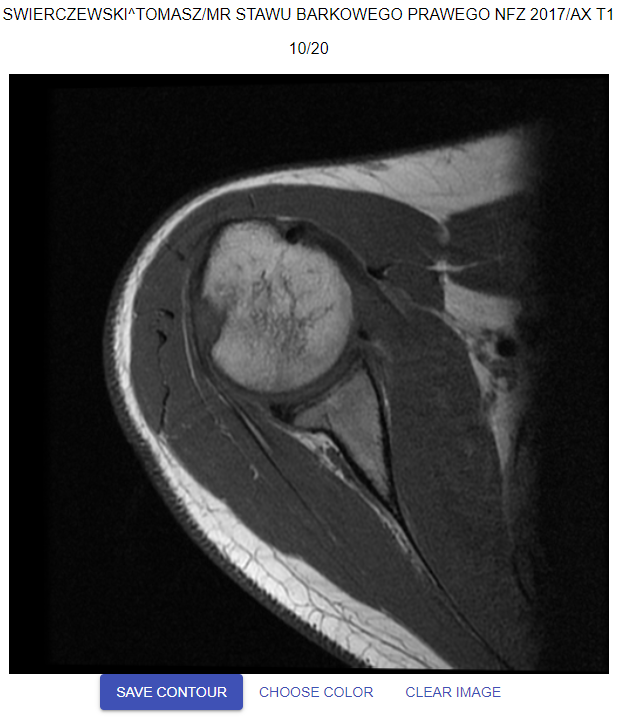
\includegraphics[width=1.0\textwidth]{140}
	\end{center}
	\endminipage\hfill
	\caption{Dwie kolejne warstwy badania MRI}
	\label{fig:140}
\end{center}
\end{figure}

%https://github.com/embiem/react-canvas-draw

Aplikacja ta spełnia wszystkie zakładane wymagania w~zakresie przeglądania i~obsługi różnych typów plików.
Dzięki zastosowaniu serwera Orthanc powinny być obsługiwane wszystkie pliki DICOM.

\bigskip

Aplikacja pozwala na~wykonanie obrysu na~wyświetlanym obrazie. Może to~być zarówno obrys
manualny jak i~półautomatyczny. Na Rysunku \ref{fig:105} przedstawiono przykładowy obrys manualny
wykonany na~badaniu MRI barku. Po~lewej stronie jest przedstawiony obrys, a~po~prawej 
stronie są~przedstawione statystyki ROI, czyli regionu zainteresowania, w~tym przypadku obszaru
wewnątrz obrysu.

Na tym badaniu jest przedstawiony bark prawy i~dokonano obrysu kości ramiennej. W~statystykach można
znaleźć takie informacje jak obwód, pole powierzchni ROI, jego środek na obrazie. Dodatkowo jest zawarty
histogram, a~na nim kluczowe informacje o~luminancji w~ROI.

\pagebreak

%\begin{figure}[p]
%	\center
%	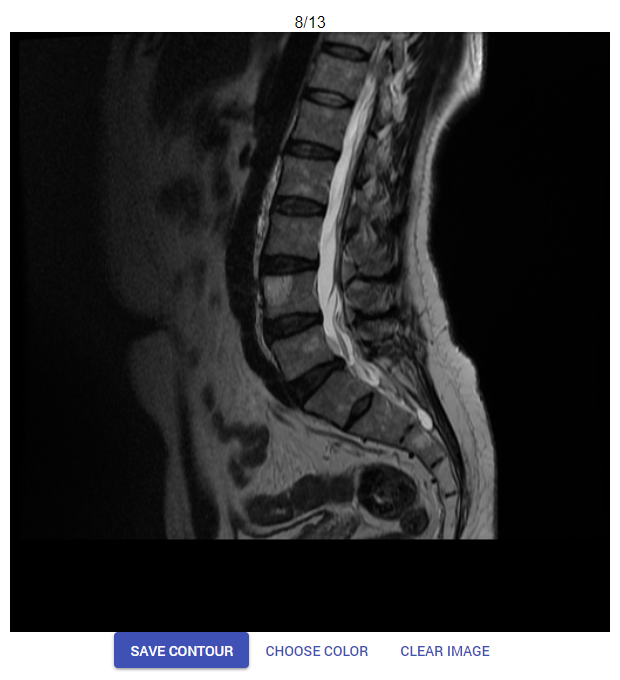
\includegraphics[width=0.6\textwidth]{114}
%	\caption{Widok badania rezonansem magnetycznego kręgosłupa}
%    	\label{fig:114}
%\end{figure}

%\begin{figure}[p]
%	\center
%	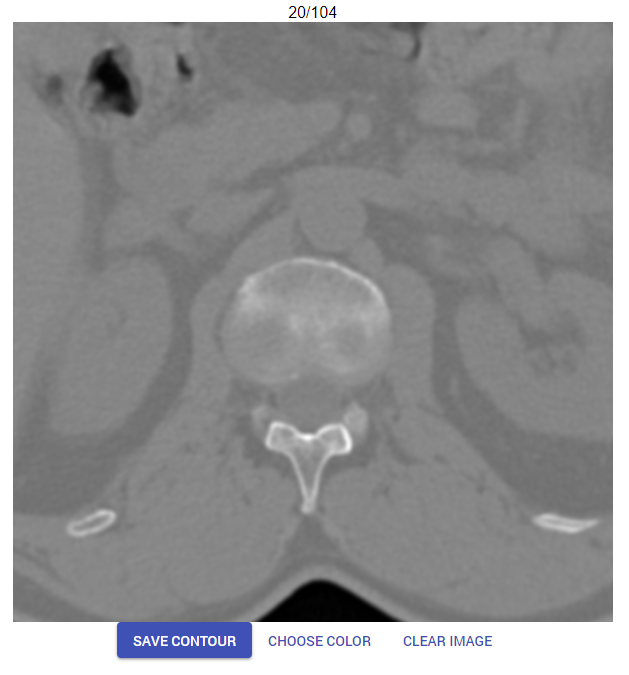
\includegraphics[width=0.6\textwidth]{115}
%	\caption{Widok badania tomografią komputerową kręgosłupa}
%    	\label{fig:115}
%\end{figure}

\begin{figure}[h!]
	\center
	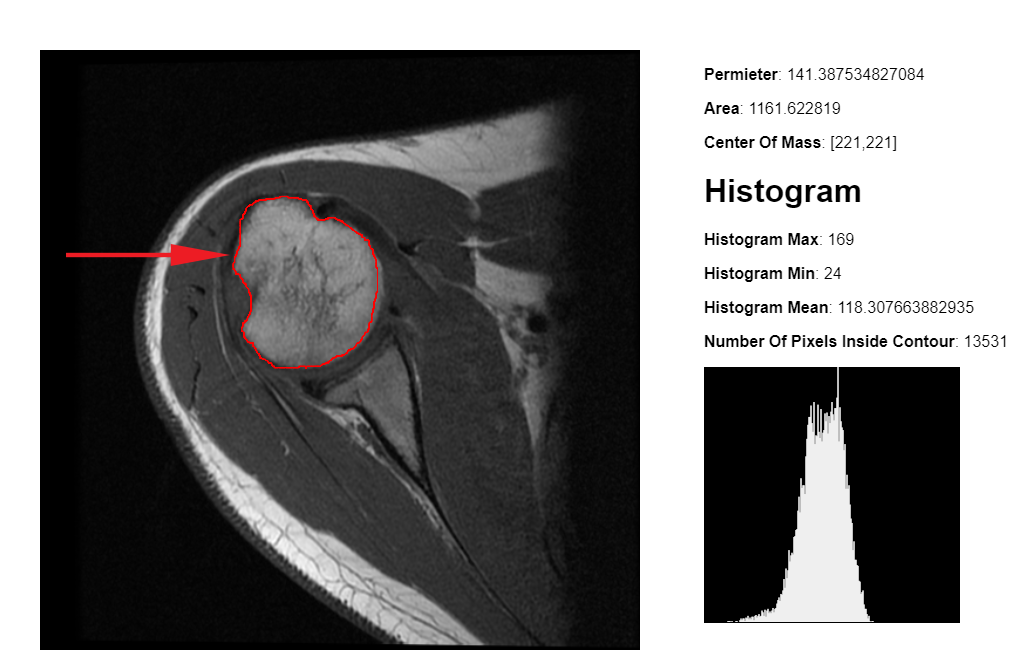
\includegraphics[width=0.9\textwidth]{105b}
	\caption{Przykładowy obrys manualny na MRI barku wraz z~wyznaczonymi statystykami}
    	\label{fig:105}
\end{figure}

Na~tym samym badaniu wykonano test obrysu półautomatycznego i~przedstawiono
go~na~Rysunku \ref{fig:107}. Analogicznie wygenerowany obrys znajduje się po lewej stronie,
a~statystyki po~prawej.

\begin{figure}[h!]
	\center
	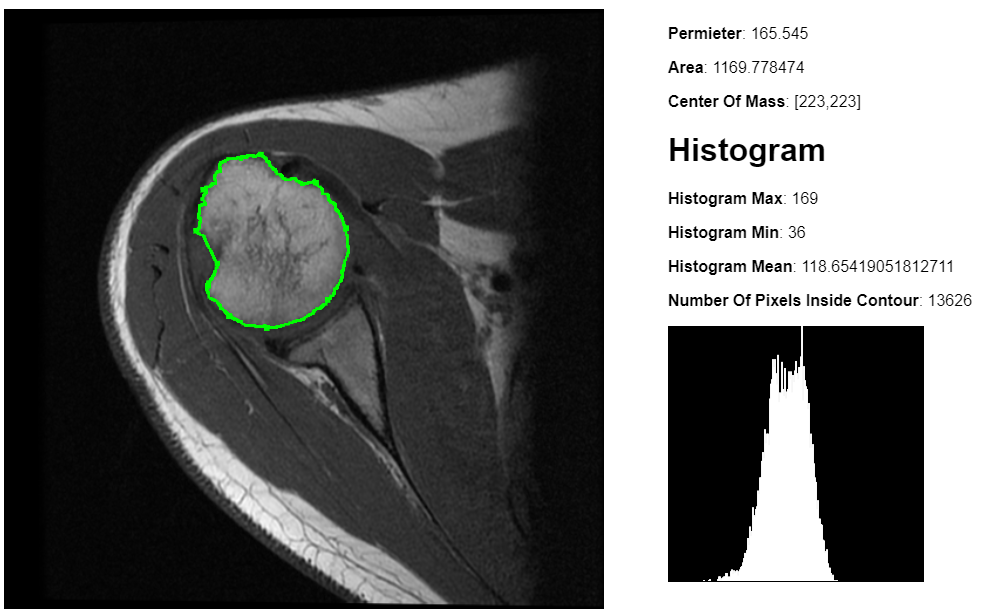
\includegraphics[width=0.9\textwidth]{107}
	\caption{Przykładowy obrys półautomatyczny na MRI barku
	wraz z~wyznaczonymi statystykami}
    	\label{fig:107}
\end{figure}

\pagebreak

W ramach analizy działania aplikacji wykonano test edycji obrysu półautomatycznego w~trakcie
jego tworzenia. Przebieg tego testu przedstawiono na~Rysunku \ref{fig:146}.

\begin{figure}[h!]
\begin{center}
	\minipage{0.24\textwidth}
	\begin{center}
		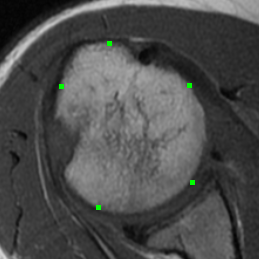
\includegraphics[width=1.0\textwidth]{146}
		a
	\end{center}
	\endminipage\hfill
	\minipage{0.24\textwidth}
	\begin{center}
		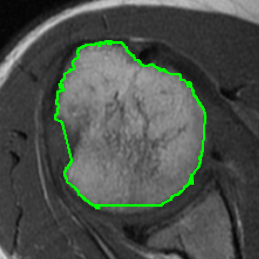
\includegraphics[width=1.0\textwidth]{147}
		b
	\end{center}
	\endminipage\hfill
	\minipage{0.24\textwidth}
	\begin{center}
		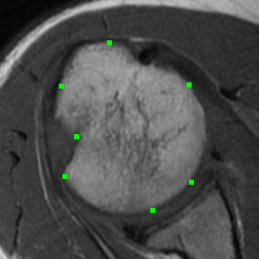
\includegraphics[width=1.0\textwidth]{148}
		c
	\end{center}
	\endminipage\hfill
	\minipage{0.24\textwidth}
	\begin{center}
		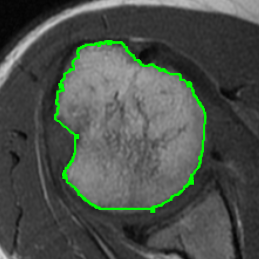
\includegraphics[width=1.0\textwidth]{149}
		d
	\end{center}
	\endminipage\hfill
	\caption{Przykład edycji obrysu półautomatycznego. Początkowo wybrano pięć punktów 
	(a)~i~wygenerowano obrys (b). Następnie usunięto jeden z~punktów i~dodano dwa kolejne (c). 
	Wygenerowany w~ten sposób obrys półautomatyczny (d).}
	\label{fig:146}
\end{center}
\end{figure}

\section {Wydajność algorytmu półautomatycznego}

W celu sprawdzenia wydajności stworzonego algorytmu półautomatycznego posłużono
się badaniem MRI barku, o~rozdzielczości 512 na~512 pikseli. Widok tego badania został przedstawiony
na Rysunku \ref{fig:112}.

\begin{figure}[h!]
	\center
	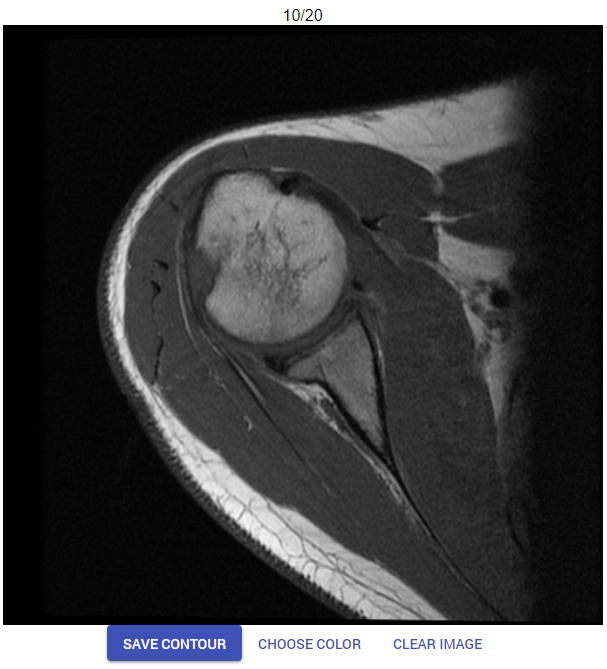
\includegraphics[width=0.5\textwidth]{112}
	\caption{Widok badania MRI barku, na którym wykonywano testy}
    	\label{fig:112}
\end{figure}

\pagebreak

W pierwszym teście sprawdzono czasy generowania obrysu półautomatycznego,
 w~zależności od~ilości punktów wybranych przez użytkownika. Oczekiwano,
że obrys będzie wyglądał podobnie do~tych na~Rysunkach \ref{fig:105} i~\ref{fig:107}.
Rozmiary przetwarzanych fragmentów obrazu w~algorytmie były porównywalne. Algorytm
wykorzystywał fragmenty obrazu medycznego zawierające wszystkie punkty wybrane
przez użytkownika z~uwzględnieniem marginesów.

W trakcie dodawania kolejnych punktów starano się poprawiać obrys, tzn. aby
wygenerowany obrys jak najlepiej odwzorowywał granicę kości. Przy okazji dodawania kolejnych
punktów do~tego samego obrysu przetestowano funkcjonalność dodawania kolejnych
punktów do~obrysu.

Dla każdej liczby wierzchołków przeprowadzano 10~kolejnych pomiarów generowania
tego samego obrysu. Pozwoliło to~na~wyznaczenie średniego czasu generowania obrysu,
niezależnie od~chwilowego wykorzystania procesora. Średni czas był obliczany przez narzędzia 
programistyczne badając działanie serwera w trybie debugowania. Realizowano to~przez
analizę czasu potrzebny na wygenerowanie odpowiedzi przez serwer.

Większość z~generowanych obrysów było podglądami, czyli nie obliczano dla nich
statystyk. Czas mierzono poprzez sprawdzanie czasu potrzebnego na~wygenerowanie
odpowiedzi przez API na~otrzymane zapytanie.

\begin{figure}[h!]
	\center
	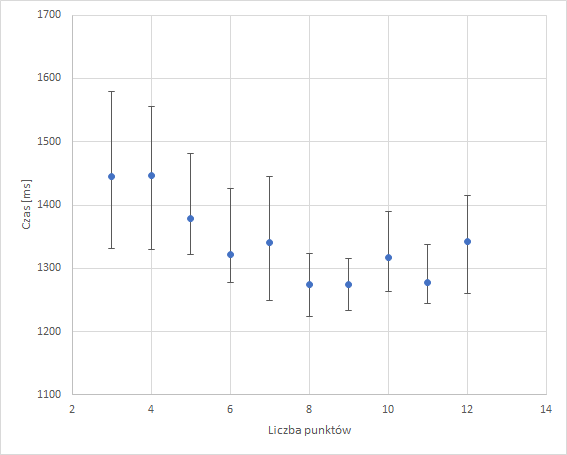
\includegraphics[width=0.85\textwidth]{152}
	\caption{Czasy generowania obrysu półautomatycznego granicy kości ramiennej
	 w~zależności od~liczby punktów
	początkowych wskazanych przez użytkownika}
    	\label{fig:testy_1}
\end{figure}

Na Rysunku \ref{fig:testy_1} przedstawiono wyniki przeprowadzonych testów. Wraz
z dodawaniem kolejnych punktów zmniejszał się czas potrzebny na~wygenerowanie
obrysu przez serwer. Warto zauważyć, że wartości zmniejszyły się o~ok. 150ms.
Nie dodawano kolejnych punktów z~uwagi na~osiągnięcie zadowalającej jakości
wygenerowanego obrysu.

\begin{figure}[h!]
	\center
	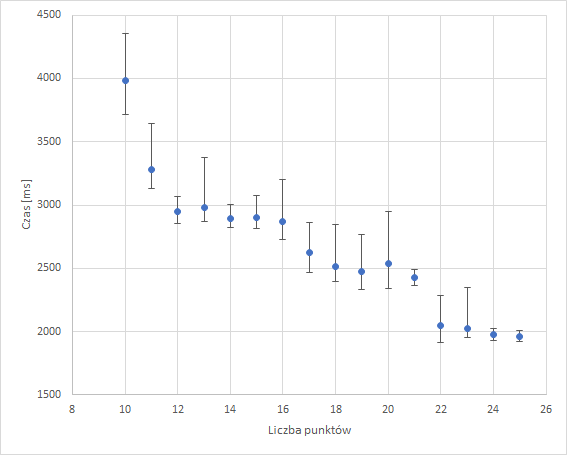
\includegraphics[width=0.85\textwidth]{151}
	\caption{Czasy generowania obrysu półautomatycznego barku w~zależności od~liczby punktów
	początkowych wskazanych przez użytkownika dla równomiernego wstawiania punktów}
    	\label{fig:testy_2}
\end{figure}


%Na Rysunku \ref{fig:testy_2} przedstawiono wyniki dla drugiego z~testów. Starano się obrysować
W kolejnym teście (Rysunek \ref{fig:testy_2}) obrysowano
cały brak widoczny na~obrazie medycznym. W~tym celu wstawiano kolejne
punkty i~obserwowano czasy, jakie były potrzebne na~wygenerowanie obrysu. Wraz z
kolejnymi punktami poprawiano generowany obrys. Czasy generowania zmalały prawie 2~krotnie, z~poziomu
około 4s~do~około 2s.

%\begin{figure}[h!]
%	\center
%	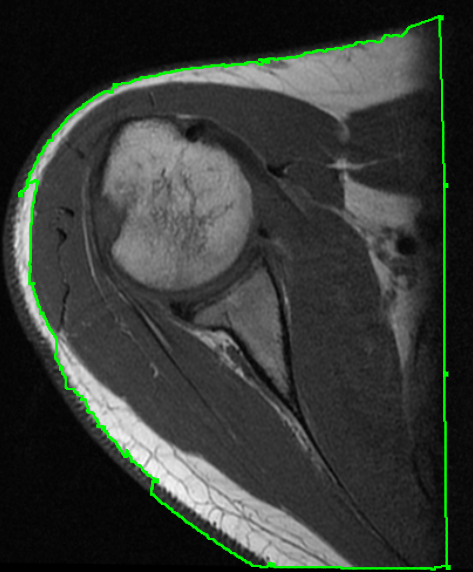
\includegraphics[width=0.6\textwidth]{108}
%	\caption{Jeden z~wygenerowanych obrysów w~trakcie testów}
%    	\label{fig:108}
%\end{figure}


Na Rysunku \ref{fig:testy_2} można zauważyć czasami gwałtowne skoki w~zmniejszającym
się czasie potrzebnym na~obliczenia. Mogło to~być spowodowane faktem, że zmieniała
się maksymalna odległość między kolejnymi punktami. Bliżej to~zjawisko zostało
opisane w~podrozdziale 4.4.

\begin{figure}[h!]
	\center
	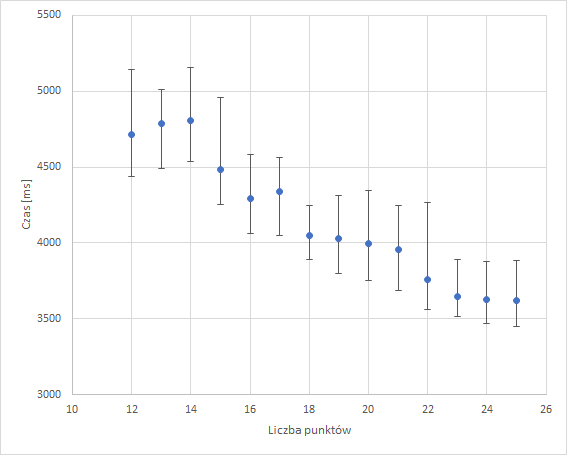
\includegraphics[width=0.85\textwidth]{150}
	\caption{Czasy generowania obrysu półautomatycznego barku w~zależności od~ilości punktów 
	w~celu analizy zależności od algorytmu A*}
    	\label{fig:testy_3}
\end{figure}

Na Rysunku \ref{fig:testy_3} przedstawiono wyniki trzeciego testu. Nie ingerowano
we wspomnianą w~podrozdziale 4.4 maksymalną odległość --- wstawiano gęsto kolejne
punkty obok siebie na~łuku. W~ten sposób sprawdzano wpływ liczby uruchomień
algorytmu A* poprzez zmianę liczby punktów na~czas obliczeń.

Uzyskane wyniki są bardzo podobne do~poprzednich, choć bez wyraźnych skoków.
Czas potrzebny na~wygenerowanie obrysu nie spadł tak bardzo jak w~drugim teście,
ale spadek był zauważalny, z~ok. 4.7s~do~3.7s. 

Wraz ze~zwiększeniem się przestrzeni roboczej obrazu rośnie czas potrzebny na
wygenerowanie obrysu. Na~podstawie wykresów zależności czasu od~liczby punktów
można wysnuć wnioski, że lepiej jest stawiać więcej punktów, niż mniej. Ponadto na czas generowania
obrysu półautomatycznego wpływa zarówno przestrzeń robocza, jak i~liczba wywołań algorytmu A*. Gdy zwiększamy
liczbę punktów, to~zarówno algorytm A* szybciej znajdzie kolejny punkt zaznaczony przez użytkownika, jak i~nie
trzeba analizować dużej części obrazu.

\section {Analiza wyników i~wnioski}

%Poniżej przedstawiono analizę wyników oraz wnioski z~przeprowadzonych testów.

Na podstawie przeprowadzonych testów
zauważono, że gdy są generowane statystyki, to~czas potrzebny na~obliczenie statystyk
zwiększał czas na~realizację zapytania o~około 30\%. Wiązało się to~z~odwiedzeniem
wszystkich punktów wewnątrz obrysu, co~powodowało wydłużenie obliczeń.

Wraz ze~zwiększaniem rozdzielczości obrazu, jak również ze~zwiększeniem się
tworzonego obrysu na~obrazach medycznych o~wysokiej rozdzielczości, wzrastał proporcjonalnie
czas potrzebny na~wygenerowanie obrysu półautomatycznego. Dzieje się tak dlatego,
że w~algorytmie wykorzystano operator Sobela i~Canny'ego, które wymagają odwiedzenia
pewnej liczby pikseli, która odpowiednio się zwiększa. Dla mammogramów, które miały rozdzielczość
blisko 20 megapikseli, obrys był generowany nawet kilkadziesiąt sekund. Dla większości obrysów
czasy obliczeń nie przekraczały zakładanych 30~sekund w~wymaganiach niefunkcjonalnych.

Ponadto warto podkreślić, że~wraz 
ze~zwiększaniem liczby punktów zmniejszał się czas potrzebny na~wygenerowanie
obrysu półautomatycznego. Powodowały to~dwa oddzielne zjawiska. Pierwsze z~nich, to
maksymalna odległość pomiędzy kolejnymi dwoma punktami wybranymi przez użytkownika.
W celu zapewnienia spójności grafu dodawano sztuczne krawędzie, o~maksymalnej długości
nieprzekraczającej maksymalnej odległości pomiędzy wcześniej wspomnianymi punktami.
Im krótsza była to~odległość, tym mniej było dodawanych sztucznych krawędzi.
Dodawanie nowych krawędzi pomiędzy oddalonymi od~siebie punktami oznaczało
kilkukrotnie mniejszą liczbę przetwarzanych krawędzi przetwarzanych przez algorytm
A*. Drugim zjawiskiem odpowiedzialnym za~zmniejszanie się czasu potrzebnego na
wygenerowanie obrysu półautomatycznego, wraz z~zwiększającą się liczbą punktów,
był algorytm A*. Początkowo przypuszczano, że zwiększanie liczby uruchomień algorytmu
A* wraz ze~wzrostem liczby punktów będzie generował dodatkowy koszt obliczeniowy,
a~nie go~redukował. Tak może się stać w~pesymistycznym przypadku. W~realnych
obrysach wraz z~dodawaniem kolejnych punktów w~celu poprawienia jakości obrysu
malała złożoność średnia, ponieważ algorytm A* szybciej znajdował prawidłową
ścieżkę. Algorytm A* dzięki heurystyce pomijał bardzo dużą liczbę krawędzi,
które na~pewno nie polepszyłyby rozwiązania.

Wraz ze~wzrostem liczby punktów wybranych przez użytkownika najczęściej malał
czas potrzebny na~wygenerowanie obrysu półautomatycznego. Czas dla większych
obrysów malał w~sposób znaczący, dla małych obrysów w~sposób niezauważalny.
Działo się tak dlatego, że operacje na~grafach były tylko elementem obliczeń. W
przypadku małych obrysów, dominującą częścią obliczeń były operacje na~przetwarzanym
obrazie. Ponadto czasy obliczeń zawierają narzut czasowy wywołany przez
przetwarzanie zapytań.

W~przypadku zdjęć o wysokiej rozdzielczości, takich jak mammogramy lub badania 
rentgenowskie, autorskie narzędzie do~generowania obrysów półautomatycznych
będzie stosunkowo długo wykonywało obliczenia, rzędu kilkunastu do~kilkudziesięciu
sekund. Można uznać to za wadę. Rozwiązaniem dla tego problemu może być 
preprocessing, czyli zawężenie ROI --- regionów zainteresowania na~tych plikach
w~taki sposób, aby algorytm nie przetwarzał zbyt dużej liczby pikseli.
Ponadto generowanie obrysów
półautomatycznych działa zauważalnie lepiej dla zdjęć o~ostrych krawędziach i~o
niskim szumie. W~celu poprawienia zarówno jakości wykrywanego obrysu jak i
wydajności czasowej przeprowadzanych w~trakcie generowania obrysu obliczeń użytkownik
powinien wybierać liczbę punktów rzędu kilkunastu punktów, co~może mieć zauważalnie
lepszą wydajność niż wybranie kilku punktów.

%\afterpage{\blankpage}
\chapter {Podsumowanie}


Cel pracy został osiągnięty. Spełniono wszystkie wymagania funkcjonalne i~niefunkcjonalne,
z wyłączeniem wymagania dotyczącego wydajności generowania obrysu półautomatycznego
dla obrazów DICOM o~dużej rozdzielczości (ponad 1000000 pikseli).

W trakcie pracy nad systemem napotkano różne problemy i~ograniczenia, przede wszystkim
związane ze~specyfikacją obrazowych badań medycznych.

W interfejsie ograniczeniem okazał się dostępny rozmiar ekranu. Projektowanie
aplikacji zakładało wykorzystanie ekranu o~rozdzielczości 1920x1080, a~więc ekranu
panoramicznego. Niestety obrazy DICOM mają bardzo zróżnicowane układy --- są obrazy
kwadratowe, pionowe oraz poziome. Założenie, że ekran użytkownika jest ekranem
1920x1080 sprawia, że obrazy pionowe będą wyświetlane jedynie w~niewielkiej
części obszaru przeznaczonego dla obrazów. Jest to~niestety ograniczenie, którego
nie da~się zlikwidować, gdyż przy założeniu rozdzielczości 1080x1920 powoduje
analogiczny problem z~obrazami poziomymi. Zaleca się skonfigurowanie aplikacji
ze względu na~rodzaj badań jakie będą występowały w~systemie (MRI, RTG, MMG, itd.).


Podstawowym problemem występującym w~trakcie implementacji rozwiązania było
ustalanie kontraktów w~warstwie komunikacyjnej. Ze~względu na~niewielką ilość
akcji w~komunikacji nie zdecydowano się na~zastosowanie generatora kontraktów,
ale zaleca się wprowadzenie takiego rozwiązania ponownie w~trakcie dalszego rozwoju narzędzia.
W zależności od~złożoności komunikacji generator kontraktów może zdecydowanie
usprawnić wprowadzanie zmian w~aplikacji.

Podczas projektowania systemu zdecydowano, że obrazy DICOM będą wyświetlane w
największej rozdzielczości umożliwiającej wyświetlenie całego obrazu na~ekranie.
W związku z~tym, większość obrazów wyświetlona jest w~rozmiarze różnym od
faktycznego rozmiaru obrazu. Rozważano dwie możliwości rozdzielczości wykonywanych
obrysów: realne wymiary obrazu oraz rozmiary obrazu wyświetlanego na~ekranie.
Zdecydowano, że obrysy powinny być zapisywane w~wymiarach identycznych realnym
rozmiarom obrazu. Decyzja została uzasadniona potrzebą zapewnienia poprawnego
obliczania statystyk. Zapisywanie obrysów w~takich wymiarach ułatwia obliczanie
liczby pikseli wewnątrz obrysu.

Ze względu na~złożoność algorytmu używanego do~wyznaczania obrysu półautomatycznego,
wykonywanie obrysów półautomatycznych w~obrazach o~dużej rozdzielczości przekracza
dwukrotnie dopuszczalny czas 30~sekund. Czas
obliczeń można poprawić poprzez ograniczenie obszaru, w~którym wykrywane będą
krawędzie, ale nie rozwiąże to~problemu z~wykonywaniem obrysów o~wymiarach
zbliżonych do~pełnych wymiarów obrazu.

Podczas pracy nad narzędziem rozważano dodatkowe funkcjonalności, które nie zostały
poruszone w~tej pracy. Są one potencjalnymi możliwościami rozwoju narzędzia
stworzonego w~ramach tej pracy. Funkcjonalności te opisano szczegółowo poniżej.

W obecnej wersji systemu nie zaimplementowano deskryptorów kształtu obrysu.
Zaimplementowanie takich deskryptorów mogłoby dostarczyć dodatkowych informacji
na temat wykonanych przez użytkownika obrysów. Taka informacja może w~przyszłości
dostarczyć dodatkową zmienną, którą można by~wykorzystywać w~celu trenowania
sztucznej inteligencji w~zautomatyzowanym wykrywaniu organów, jak również wykrywaniu
i sugerowaniu niepokojących zmian.

W tej wersji w~systemie użytkownicy nie są rozróżnialni. Dodanie użytkowników
pozwoliłoby na~segregowanie tworzonych obrysów i~wyświetlanie użytkownikowi
obrysów wykonanych jedynie przez niego samego, a~nie wszystkich obrysów istniejących
w systemie. Z~punktu widzenia użyteczności systemu użytkownik nie musiałby szukać
swojego obrysu pośród obrysu innych użytkowników systemu.

Uwierzytelnianie zapobiegłoby również niepowołanemu dostępowi osób postronnych
do wykonanych obrysów oraz uniemożliwiłoby ataki typu DoS. W~obecnej wersji można
poprzez wysyłanie dużej liczby zapytań związanych z~generowaniem obrysów półautomatycznych
doprowadzić do~niedostępności przeprowadzania akcji na~serwerze. System jest również
podatny na~złośliwe działanie mające na~celu zapełnienie całej dostępnej serwerowi
przestrzeni dyskowej, które może zostać wywołane przez wysłanie dużej liczby
zapisów obrysów manualnych.

Z punktu widzenia użytkownika interesujące mogą być informacje wyliczone przez
system na~temat wykonanych przez niego obrysów. W~obecnej wersji systemu, jeśli
użytkownik chciałby takie informacje zapisać musiałby samodzielnie przepisać dane
wyświetlane w~widoku szczegółów obrysu. Zautomatyzowanie takiej funkcjonalności
mogłoby zaoszczędzić użytkownikowi wiele czasu.

Głównym celem wykonywania obrysów na~obrazach medycznym jest generowanie zbioru
testowego dla różnych metod sztucznej inteligencji mających na~celu sugerowanie
lekarzom niepokojących zmian wykrytych automatycznie. W~związku z~tym użytecznym
rozszerzeniem funkcjonalności systemu byłoby zintegrowanie go~z~modułem sztucznej
inteligencji i~umożliwienie obrysowywania wgrywanych obrazów metodami sztucznej
inteligencji opartych na~obrysach wykonanych przez użytkownika.

%\chapter*{}
%\markboth{}{}
%\addcontentsline{toc}{chapter}{}



% -------------------- 6. Bibliografia -----------------------
% Bibliografia leksykograficznie wg~nazwisk autorów
% Dla ambitnych - można skorzystać z~BibTeX-a

\begin{thebibliography}{24}%jak ktoś ma~więcej książek, to~niech wpisze większą liczbę
% \bibitem[numerek]{referencja} Autor, \emph{Tytuł}, Wydawnictwo, rok, strony
% cytowanie: \cite{referencja1, referencja 2,...}
%\chapter*{Bibliografia}
\phantomsection
\markboth{}{Bibliografia}
\addcontentsline{toc}{chapter}{Bibliografia}


\bibitem{Redux} Abramov D. and the Redux documentation authors: ReduxJs https://redux.js.org/ [Dostęp 1~kwietnia 2019]
\bibitem{C w pigulce} Albahari J., Albahari B. "C~6.0 w~pigułce", \emph{Helion, O'Reilly Media, Inc.}, Gliwice,  2016
\bibitem{React canvas draw} Beierling-Mutz M. React Canvas Draw. Oficjalne repozytorium: https://github.com/embiem/react-canvas-draw [Dostęp 1~kwietnia 2019]
\bibitem{Bresenham} Bresenham J. E. "Algorithm for computer control of~a~digital plotter." \emph{ICM System Journal 4(1)} 1965
\bibitem{AiSD2} Bródka J. Wykłady z~przedmiotu Algorytmy i~Struktury Danych 2~\emph{Politechnika Warszawska, Wydział Matematyki i~Nauk Informacyjnych} Materiały dostepne na~stronie: http://mini.pw.edu.pl/~brodka/ASD2.html [Dostęp 1~kwietnia 2019]
\bibitem{Canny} Canny J. F. "Finding Edges and Lines in~Images." \emph{Technical report no. 720, Massachusetts Institute of~Technology (MIT)}, Cambridge, Massachusetts, USA, 1983
\bibitem{Cyfrowe przetwarzanie obrazów medycznych} Cytowski J., Gielecki J., Gola A. "Cyfrowe przetwarzanie obrazów medycznych: Algorytmy. Technologie. Zastosowania." \emph{Akademicka Oficyna Wydawnicza EXIT}, Warszawa, 2008
\bibitem{React} Facebook Inc.: Informacje o~bibliotece ReactJS. Oficjalna strona: https://reactjs.org/ [Dostęp 1~kwietnia 2019]
\bibitem{SonicDICOM} JIUN Corporation: Oficjana strona: https://sonicdicom.com/ [Dostęp 24~marca 2019]
\bibitem{SonicDICOM} JIUN Corporation: Przykład użycia intefejsu podglądu badań w systemie SonicDICOM: https://sonicdicom.com/screens/viewer-of-dicom-viewer/ [Dostęp 24~marca 2019]
\bibitem{SonicDICOM API} JIUN Corporation: Instrukcja korzystania z~REST API SonicDICOM. Oficialna strona: https://docs.sonicdicom.com/install-manual/integration.html [Dostęp 24 marca 2019]
\bibitem{Cornerstone Core} Hafey C. Dokumentacja projektu Cornerstone Core. Oficjalna strona: https://docs.cornerstonejs.org/ [Dostęp 1~kwietnia 2019]
\bibitem{Cornerstone Tools} Hafey C. Dokumentacja projektu Cornerstone Tools. Oficjalna strona: https://tools.cornerstonejs.org/ [Dostęp 1~kwietnia 2019]
\bibitem{A*} Hart P. E., Nilsson N. J., Raphael B. "A~Formal Basis for the Heurestic Determination of~Minimum Cost Paths" \emph{IEEE Transactions on~Systems Science and Cybernetics 4(2)}, 1968
\bibitem{DWV} ivmartel: Projekt DICOM Web Viewer. Oficjalna strona: https://ivmartel.github.io/dwv/ [Dostęp 1~kwietnia 2019]
\bibitem{Dlaczego dotnet} Kronis K., Uhanova M. "Performance Comparision of~Java EE~and ASP.NET Core Technologies for Web API Developmnet." \emph{Applied Computer Systems 23, Riga Technical University}, Ryga, 2018
\bibitem{Dotnet} Microsoft Corporation: Dokumentacja platformy .NET. Oficjalna strona: https://docs.microsoft.com/pl-pl/dotnet/ [Dostęp 1~kwietnia 2019]
\bibitem{Dotnet struktury} Microsoft Corporation: Dokumentacja rekomendowanych struktur danych platformy .NET. Oficjalna strona: https://docs.microsoft.com/pl-pl/dotnet/standard/collections/ [Dostęp 1~kwietnia 2019]
\bibitem{Charakterystyka dotnet} Microsoft Corporation: Informacje o~platformie .NET Core. Oficialna strona: https://docs.microsoft.com/pl-pl/dotnet/core/about [Dostęp 1~kwietnia 2019]
\bibitem{ASPNET} Microsoft Corporation: Informacje o~platformie ASP.NET Core. Oficialna strona: https://docs.microsoft.com/pl-pl/aspnet/core/?view=aspnetcore-2.2 [Dostęp 1~kwietnia 2019]
\bibitem{Canvas} Mozilla and individual contributors: Dokumentacja HTMLCanvasElement. Oficjalna strona: https://developer.mozilla.org/en-US/docs/Web/API/HTMLCanvasElement/ [Dostęp 1~kwietnia 2019]
\bibitem{DICOM} National Electrical Manufacturers Association: Standard DICOM. Oficjalna strona: https://www.dicomstandard.org/ [Dostęp 1~kwietnia 2019]
\bibitem{Dlaczego react} Nowacki R., Plechawska-Wójcik M. "Analiza porównawcza narzędzi do~budowania aplikacji Single Page Application --- AngularJS, ReactJS, Ember.js" \emph{Journal of~Computer Sciences Institute 2, Politechnika Lubelska, Instytut Informatyki}, Lublin, 2016
\bibitem{OHIF Viewer} OHIF: Open Health Imaging Foundation. Oficjalna strona: http://ohif.org/ [Dostęp 1~kwietnia 2019]
\bibitem{Orthanc} Osimis S.A.: Projekt Orthanc. Oficjalna strona: https://www.orthanc-server.com/ [Dostęp 1~kwietnia 2019]
\bibitem{Orthanc API} Osimis S.A.: Instrukcja korzystania z~REST API Orthanc. Oficjalna strona: http://book.orthanc-server.com/users/rest.html [Dostęp 1~kwietnia 2019]
\bibitem{Pixel connectivity} Rosenfeld A., Kak A. C. "Digital Picture Processing" \emph{Academic Press, Inc.}, Nowy Jork, 1982
\bibitem{KMM} Saeed K., Rybnik M., Tabędzki M., Adamski M. "Algorytm do~Ścieniania Obrazów: Implementacja i~Zastosowania" \emph{Zeszyty Naukowe Politechniki Białostockiej 2002 Informatyka - Zeszyt 1}, Białystok, 2002
\bibitem{K3M} Saeed K., Tabędzki M., Rybnik M., Adamski M. "K3M: A~Universal Algorithm for Image Skeletonization and a~Review of~Thinning Techniques" \emph{International Journal of~Applied Mathematics and Computer Science, 2010, 20(2)} Białystok, 2010
\bibitem{Algorytmy Sedgewick} Sedgewick R., Wayne K. "Algorytmy Wydanie IV", \emph{Helion}, Gliwice, 2012
\bibitem{Sobel} Sobel I., Feldman G. "An~3x3 Isotropic Image Gradient Operator for Image Processing" \emph {Presentation at~Stanford Aartificial Intelligence Project (SAIL) in~1968}, 2014
\bibitem{Moore} Weisstein, Eric W. "Moore Neighborhood" \emph{From MathWorld--A Wolfram Web Resource.} http://mathworld.wolfram.com/MooreNeighborhood.html [Dostęp 1~kwietnia 2019]

%\bibitem[1]{Ktos} A. Author, \emph{Title of~a~book}, Publisher, year, page--page.
%\bibitem[2]{Innyktos} J. Bobkowski, S. Dobkowski, Jak stworzyć bibliografię w~BibTeX-u, \emph{Czasopismo nr}, rok, strona--strona.
%\bibitem[3]{B} C. Brink, Power structures, \emph{Algebra Universalis 30(2)}, 1993, 177--216.
%\bibitem[4]{H} F. Burris, H. P. Sankappanavar, \emph{A Course of~Universal Algebra}, Springer-Verlag, Nowy Jork, 1981.
\end{thebibliography}

%\thispagestyle{empty}
%\pagenumbering{gobble}



% --- 9. Wykaz symboli i~skrótów - jeśli nie ma, zakomentować
\afterpage{\blankpage}
\chapter*{Wykaz symboli i~skrótów}
\markboth{}{Wykaz symboli i~skrótów}
\addcontentsline{toc}{chapter}{Wykaz symboli i~skrótów}


\begin{itemize}[noitemsep]
\item API -- ang. \textit{Application Programming Interface} --- zestaw ściśle określonych reguł, poprzez które komunikują się ze~sobą programy\\
\item CRUD --- ang. \textit{Create, Read, Update, Delete} --- utwórz, odczytaj, aktualizuj i~usuń -- cztery podstawowe funkcje w~aplikacjach, które umożliwiają zarządzanie nią\\
\item CSV --- ang. \textit{Comma-Separated Values} (w pracy użyte w~kontekście formatu pliku) \\
\item DoS --- ang. \textit{Denial of~Service} --- atak na~system komputerowy mający na~celu uniemożliwienie działania systemu\\
\item DICOM --- ang. \textit{Digital Imaging and Communications in~Medicine} --- norma ujednolicająca wymianę i~interpretację obrazowych danych medycznych\\
\item HTML5 --- ang. \textit{HyperText Markup Language 5} --- język do~tworzenia i~prezentowania stron internetowych www\\
\item HTTP --- ang. \textit{Hypertext Transfer Protocol} --- protokół wymiany danych hipertekstowych\\
\item HTTPS --- ang. \textit{Hypertex Transfer Protocol Secure} --- szyfrowana wersja protokołu HTTP\\
\item ID~--- ang. \textit{Identifier} --- unikalna nazwa przypisana do~danego obiektu, pozwalająca rozróżniać obiekty w~systemie\\
\item JSON --- ang. \textit{JavaScript Object Notation} --- lekki format wymiany danych, bazujący na~podzbiorze języka JavaScript\\
\item REST --- ang. \textit{Representational State Transfer} --- styl architektury oprogramowania dla systemów rozproszonych\\
\item RGB --- ang. \textit{Red, Green, Blue} --- model przestrzeni barw, opisanej współrzędnymi 3~barw podstawowych: czerwonej, zielonej i~niebieskiej\\
\item SDK --- ang. \textit{Software Development Kit} --- zestaw narzędzi programistycznych niezbędny do~tworzenia aplikacji korzystającej z~danej biblioteki\\
\end{itemize}

%\thispagestyle{empty}


%\afterpage{\blankpage}

% ----- 10. Spis rysunków - jeśli nie ma, zakomentować --------
\listoffigures
\markboth{}{Spis rysunków}
\addcontentsline{toc}{chapter}{Spis rysunków}
%\thispagestyle{empty}
%Jak nie występują, usunąć.


%\afterpage{\blankpage}


% ------------ 11. Spis tabel - jak wyżej ------------------
%\renewcommand{\listtablename}{Spis tabel}
%\phantomsection
%\markboth{}{Spis tabel}
%\addcontentsline{toc}{chapter}{Spis tabel}
%\listoftables
%\thispagestyle{empty}
%Jak nie występują, usunąć.

%---- 12. Spis CD

\chapter*{Spis zawartości załączonej płyty CD}
\markboth{}{Spis zawartości załączonej płyty CD}
\addcontentsline{toc}{chapter}{Spis zawartości załączonej płyty CD}

Do niniejszej pracy dyplomowej inżynierskiej została załączona płyta CD. W~jej skład wchodzą:
\begin{itemize}[noitemsep]
\item wersja elektroniczna pracy, której treść jest identyczna z~powyższą w
pliku \verb+garsteckil-swierczewskit-praca-inzynierska.pdf+,
\item strona tytułowa pracy w~pliku \verb+garsteckil-swierczewskit-strona-tytulowa.pdf+,
\item streszczenie w~języku polskim i~angielskim w~plikach o~nazwach odpowiednio
\verb+garsteckil-swierczewskit-stresczenie.pdf+ i~\verb+garsteckil-swierczewski-abstract.pdf+.
\end{itemize}

Kod źródłowy, który został podzielony na~kilka katalogów:
\begin{itemize}
\item \verb+DotNetProject/+ - zawierający kod źródłowy głównego serwera aplikacji.
Główne algorytmy odpowiedzialne za~generowanie obrysów półautomatycznych znajdują się w~podkatalogu \verb+Logic/+,
\item \verb+Web/+ - zawierający kod źródłowy aplikacji przeglądarkowej.
\end{itemize}

\afterpage{\blankpage}

% 13. Spis załączników - jak nie ma~załączników, to~zakomentować lub usunąć

\chapter*{Dodatek 1 --- Pseudokod generujący graf z~bitmapy}
\markboth{}{Dodatek 1 --- Pseudokod generujący graf z~bitmapy}
\addcontentsline{toc}{chapter}{Dodatek 1 --- Pseudokod generujący graf z~bitmapy}
%\begin{enumerate}
%\item Załącznik 1~- Pseudokod generujący graf z~bitmapy

\begin{verbatim}
MATRIX - macierz wejściowa z oznaczonymi krawędziami jako 1
foreach(punkt A taki, że MATRIX(A) == 1)
{
    if ( punkt A ma 1 sąsiada albo co najmniej 3 sąsiadów )
    {
        // (tzn. jest albo punktem końcowym albo węzłowym)
        wstaw punkt A do kolejki wierzchołków L_V
        while ( kolejka wierzchołków L_V niepusta )
        {
             weź wierzchołek V_1 z kolejki L_V
            usuń V_1 z kolejki L_V
            dodaj wierzchołek V_1 do grafu G
            foreach (punkt B sąsiadujący z V_1 )
             {
                if ( MATRIX(B) == 1 )
                 {
                    stwórz nową krawędź E.
                    dodaj B do E
                    ustaw wierzchołek V_1 jako początek krawędzi E
                    dodaj krawędź E do kolejki przetwarzanych krawędzi L_E
                }
                while ( L_E niepusta)
                 {
                    weź krawędź E z L_E
                    usuń E z kolejki
                    stwórz kolejkę potencjalnych punktów krawędzi E, L_P
                    weź punkt C z E
                    usuń C z E
                    dodaj punkt C do kolejki L_P
                    while ( L_P niepusta )
                    {
                        weź punkt D z L_P
                        usuń D z L_P
                        K = liczba sąsiadów D
                        if ( K == 0 lub K > 1 )
                        {
                            stwórz wierzchołek V_2, który znajduje się w D
                            do listy krawędzi wierzchołka V_2 dodaj E
                            do listy krawędzi wierzchołka V_1 dodaj E
                            ustaw wierzchołek V_2 jako koniec krawędzi E
                            dodaj krawędź E do grafu G
                            dodaj wierzchołek V_2 do kolejki L_V
                        }
                        if ( K == 1 )
                        {
                            dodaj punkt D do E
                            foreach ( punkt F sąsiadujący z D )
                            {
                                if ( MATRIX(F) == 1)
                                {
                                    dodaj F do L_P
                                }
                            }
                        }
                        MATRIX(D) = 1
                    }
                }
            }
        }
    }
}
Zwróć graf G
\end{verbatim}

% --- 8. Instrukcja instalacji
%\item Załącznik 2~- Instrukcja instalacji
\chapter*{Dodatek 2 --- Instrukcja instalacji}
\markboth{}{Dodatek 2 --- Instrukcja instalacji}
\addcontentsline{toc}{chapter}{Dodatek 2 --- Instrukcja instalacji}

W celu instalacji serwera Orthanc należy otworzyć stronę
\url{https://www.orthanc-server.com/download.php}, pobrać wersję odpowiednią dla
używanego systemu operacyjnego, a~następnie postępować zgodnie z~instrukcjami
wyświetlanymi podczas instalacji. W~celu uzyskania szczegółowych informacji
odnośnie konfiguracji należy zapoznać się z~dokumentacją znajdującą się na~stronie
\url{http://book.orthanc-server.com/users/cookbook.html}

W celu instalacji serwera obrysów i~aplikacji webowej należy skopiować pliki
znajdujące się na~płycie w~folderach Web oraz DotNetProject na~stację,
na której aplikacje te~zostaną uruchomione.

Do działania serwera obrysów wymagany jest .NET Core w~wersji 2.2 lub nowszej.
W celu instalacji .NET Core należy otworzyć stronę \url{https://dotnet.microsoft.com/download},
pobrać wersję odpowiednią dla używanego systemu operacyjnego, a~następnie
postępować zgodnie z~informacjami wyświetlanymi w~trakcie instalacji.

W celu konfiguracji serwera w~pliku DotNetProject/Api/Properties/launchSettings.json
należy wpisać jako wartość~24~linii adres i~port, na~którym serwer ma~zostać
udostępniony, jako wartość pola applicationUrl. Przykładowa poprawna wartość
linii 24~to\texttt{ "applicationUrl": "https://localhost:5001",}.

Ponadto w~pliku DotNetProject/Api/Startup.cs należy podać w~linii 33~link pod
którym dostępna jest aplikacja przeglądarkowa jako argument metody WithOrigins.
Przykładowa poprawna wartość linii 24~to
\texttt{builder => builder.WithOrigins("http://localhost:8080", "http://localhost:3000")}.

W celu uruchomienia serwera obrysów należy przejść do~skopiowanego folderu
DotNetProject/API i~wykonać w~konsoli polecenie \texttt{\$ dotnet build \&\& dotnet run}.

Do działania aplikacji przeglądarkowej wymagany jest Node w~wersji co~najmniej
9.4 oraz yarn w~wersji co~najmniej 1.10.1, aby zainstalować Node.js należy udać
się na~stronę \url{https://nodejs.org/en/download/} i~wybrać wersję odpowiadającą
systemowi, z~którego korzystamy. Postępować zgodnie ze~wskazówkami instalatora.
W celu instalacji yarn należy udać się na~stronę https://yarnpkg.com/en/docs/install
aby pobrać wersję odpowiadającą systemowi, na~którym będzie uruchamiana aplikacja
i uruchomić instalator.

W celu konfiguracji portu, na~który będzie wystawiona aplikacja webowa należy
ustawić odpowiednią liczbę w~4~linii pliku Web/express.js. Przykładowa poprawna
konfiguracja:\\
\texttt{\$ const portNumber = 3000;}

Ponadto w~celu konfiguracji aplikacji należy ustawić adresy do~API serwera obrysów
i~serwera Orthanc w~pliku Web/src/helpers/requestHelper.ts poprzez zmianę zawartośc
cudzysłowów w~pierwszych dwóch linijkach pliku. 	Przykładowa poprawna konfiguracja:\\
\texttt{export const orthancURL = "http://localhost:8042/";}\\
\texttt{export const apiURL = "https://localhost:5001/";}

W celu uruchomienia aplikacji przeglądarkowej wchodzimy do~folderu Web, w~którym
wykonujemy polecenie \texttt{\$ yarn install \&\& yarn prod}. Uwaga, tę komendę
należy uruchomić w~konsoli obsługującej skrypty w~języku bash.


% --- 8. Instrukcja użytkowania


\newpage
%\item Załącznik 2~- Instrukcja użytkowania
\chapter*{Dodatek 3 --- Instrukcja użytkowania}
\markboth{}{Dodatek 3 --- Instrukcja użytkowania}
\addcontentsline{toc}{chapter}{Dodatek 3 --- Instrukcja użytkowania}

Po otwarciu aplikacji użytkownik może przeglądać pacjentów (patients), których
badania zostały wgrane do~serwera Orthanc --- Rysunek \ref{fig:1}.

\begin{figure}[h!]
	\center
	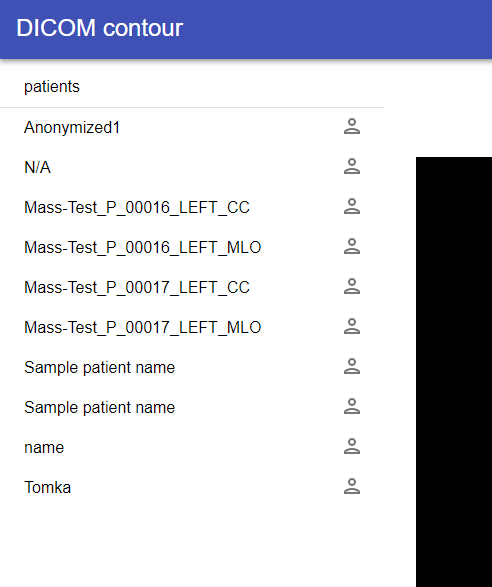
\includegraphics[width=0.6\textwidth]{1}
	\caption{Widok listy pacjentów}
    	\label{fig:1}
\end{figure}

Po wybraniu pacjenta poprzez kliknięcie lewym przyciskiem myszy na~jego nazwę,
na liście pojawiają się badania (studies) wybranego pacjenta. Użytkownik może
wrócić do~widoku pacjentów klikając w~strzałkę na~liście z~badaniami --- Rysunek \ref{fig:2}.

\begin{figure}[h!]
	\center
	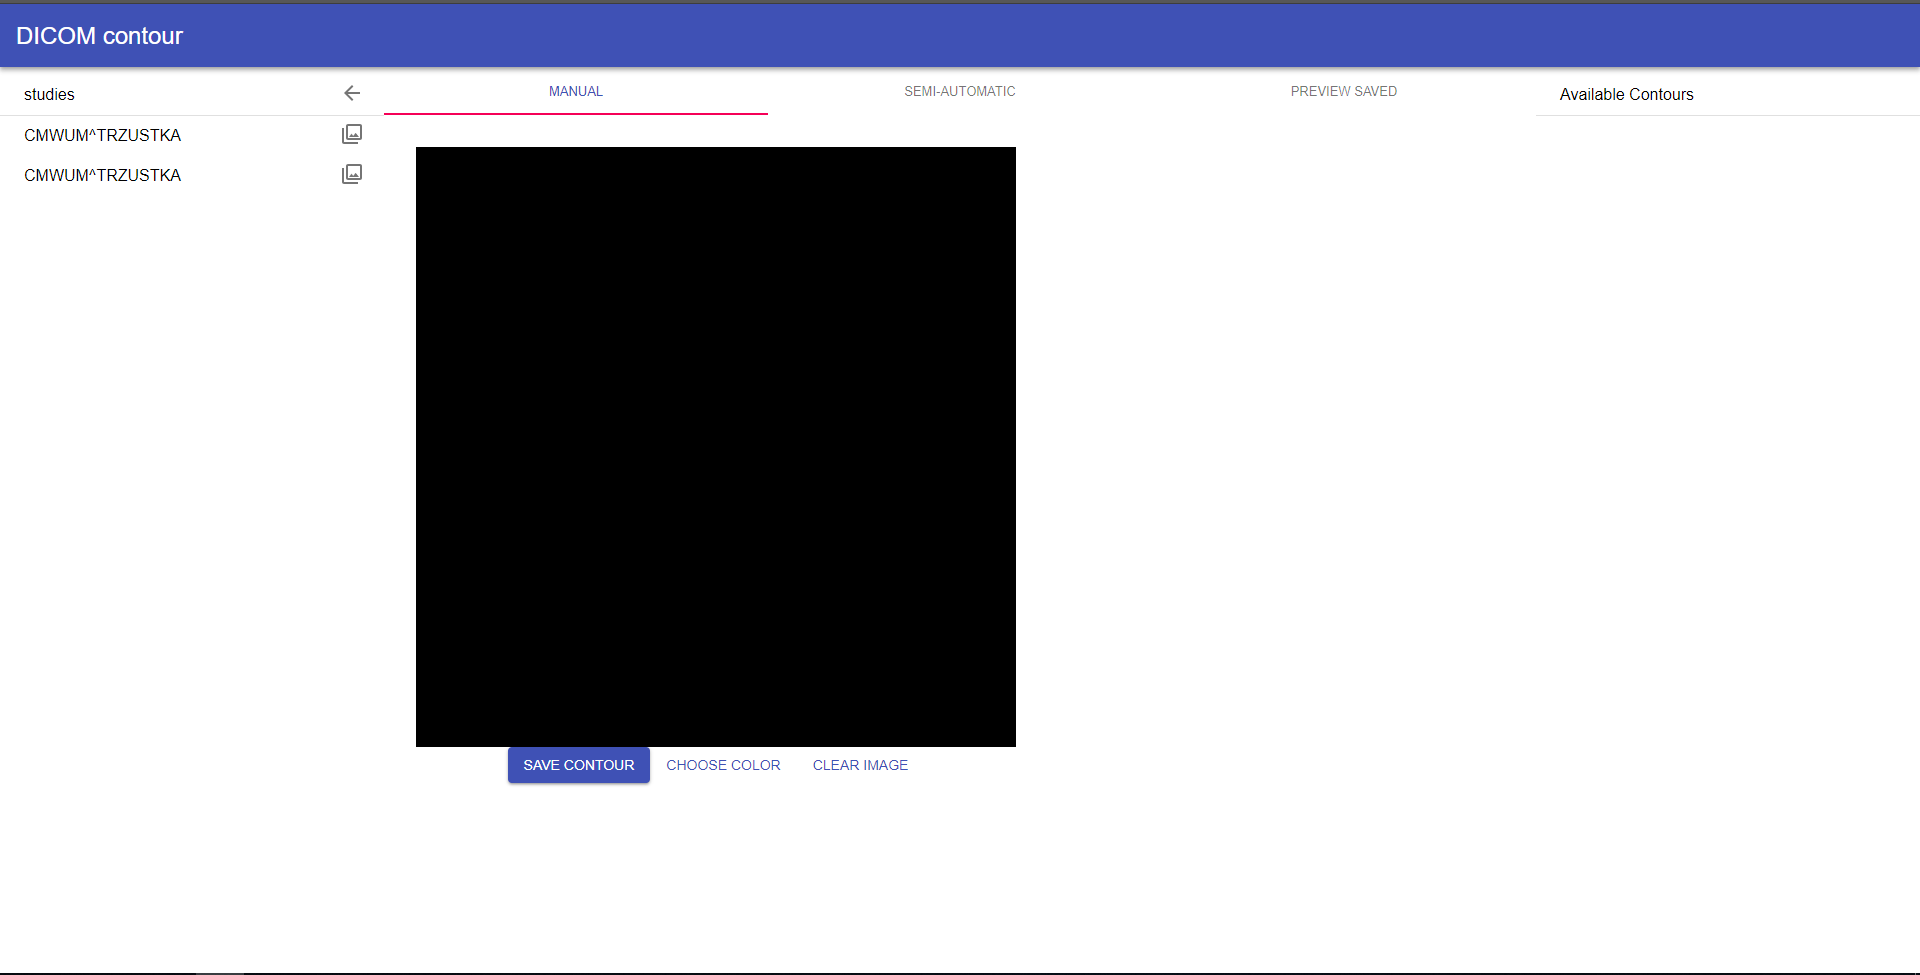
\includegraphics[width=0.6\textwidth]{2}
	\caption{Widok listy badań pacjenta}
    	\label{fig:2}
\end{figure}

\pagebreak

Po wybraniu badania poprzez kliknięcie lewym przyciskiem myszy na~jego nazwę,
na liście pojawiają się serie (series) wybranego badania. Użytkownik może wrócić
do widoku badań, klikając w~strzałkę na~liście z~seriami --- Rysunek \ref{fig:3}.

\begin{figure}[h!]
	\center
	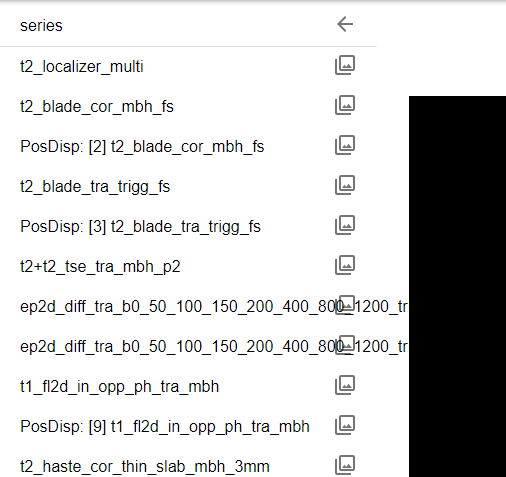
\includegraphics[width=0.7\textwidth]{3}
	\caption{Widok listy serii w~badaniu}
    	\label{fig:3}
\end{figure}

Po wyborze serii na~ekranie pojawia się pierwszy obraz z~serii. Użytkownik
może przełączać się pomiędzy obrazami korzystając z~listy obrazów po~lewej
stronie lub używając rolki myszy po~najechaniu na~obraz. Aby powrócić do~wyboru
serii należy kliknąć lewym przyciskiem myszy na~strzałkę na~liście instancji
(instances) --- Rysunek \ref{fig:4}.

\pagebreak

\begin{figure}[h!]
	\center
	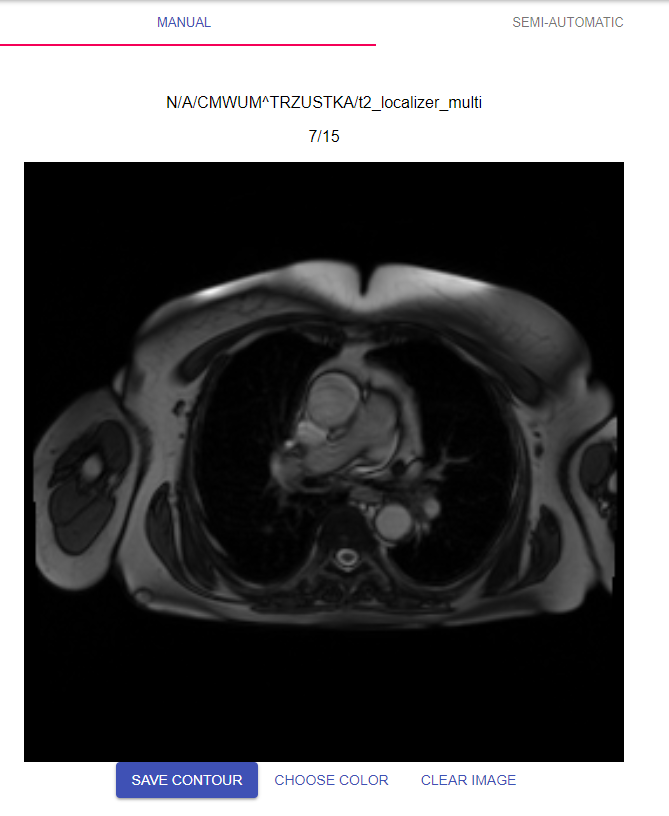
\includegraphics[width=0.5\textwidth]{4}
	\caption{Wybrany obraz w~module obrysu manualnego}
    	\label{fig:4}
\end{figure}

Przy manualnym obrysie użytkownik może wykonywać obrys poprzez przytrzymanie
lewego przycisku myszy na~obrazie, przesuwając mysz z~wciśniętym przyciskiem.
Gdy użytkownik korzysta z~tabletu graficznego wystarczy, że będzie przesuwał
wciśniętym rysikiem po~tablecie --- Rysunek \ref{fig:5}.

\begin{figure}[h!]
	\center
	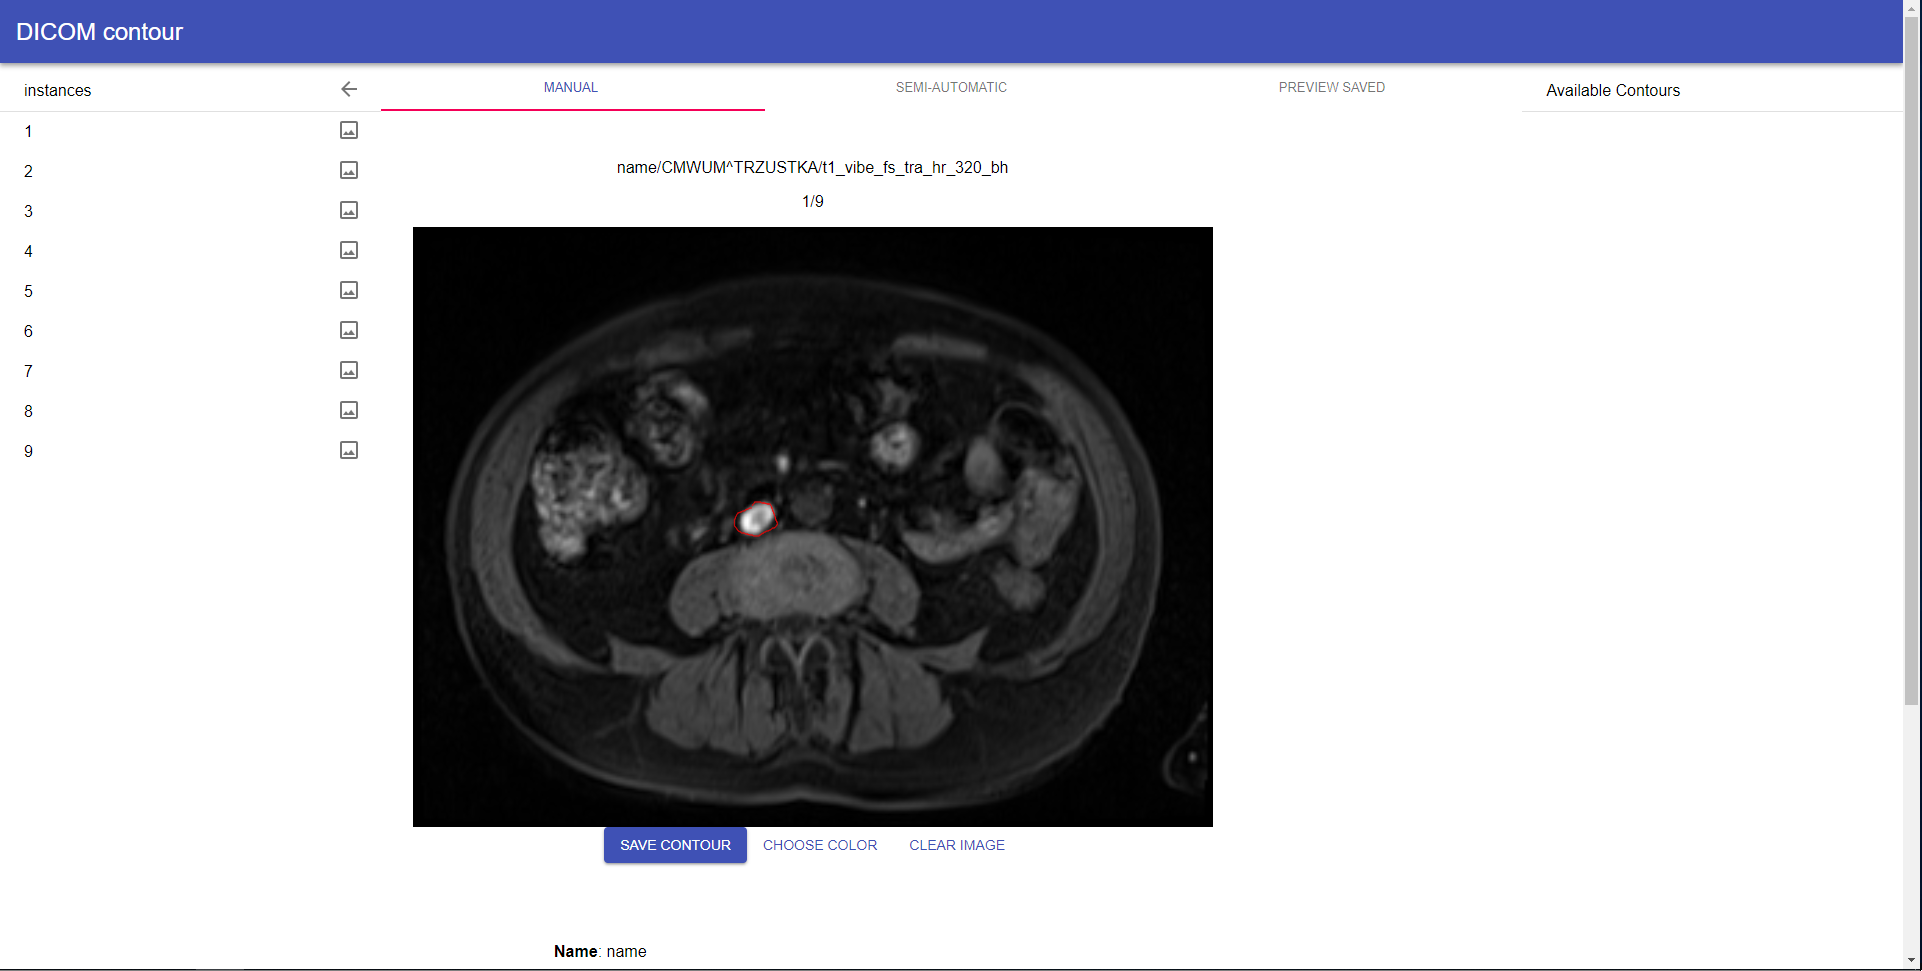
\includegraphics[width=0.8\textwidth]{5}
	\caption{Przykładowy obrys}
    	\label{fig:5}
\end{figure}

\pagebreak

W~celu usunięcia nieudanego obrysu należy kliknąć lewym przyciskiem
myszy w~przycisk wyczyść obraz (Clear Image). Po wciśnięciu przycisku zapisz obrys
(Save Contour), użytkownikowi ukazuje się okno dialogowe --- \ref{fig:6}.

\begin{figure}[h!]
	\center
	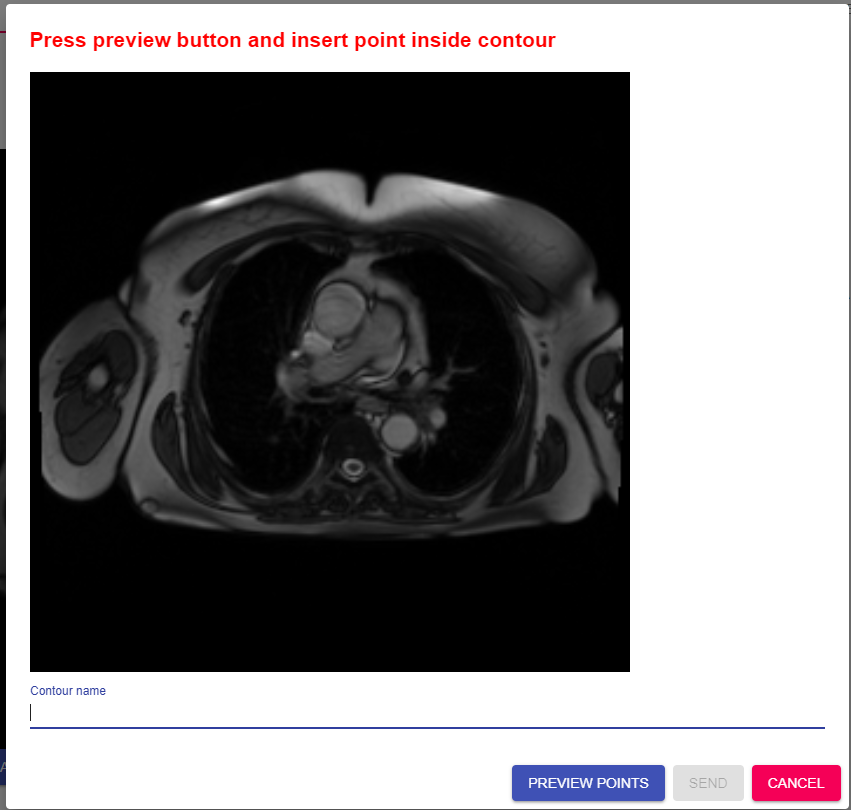
\includegraphics[width=0.48\textwidth]{6}
	\caption{Okno zapisu obrysu manualnego}
    	\label{fig:6}
\end{figure}

W~celu zapisania obrysu należy wpisać nazwę obrysu w~pole tekstowe poniżej obrazu.
Następnie, należy kliknąć przycisk podgląd punktów (Preview Points)
lewym przyciskiem myszy. Pozwoli to~użytkownikowi zobaczyć wykonany przez niego
obrys --- Rysunek \ref{fig:7}.

\begin{figure}[h!]
	\center
	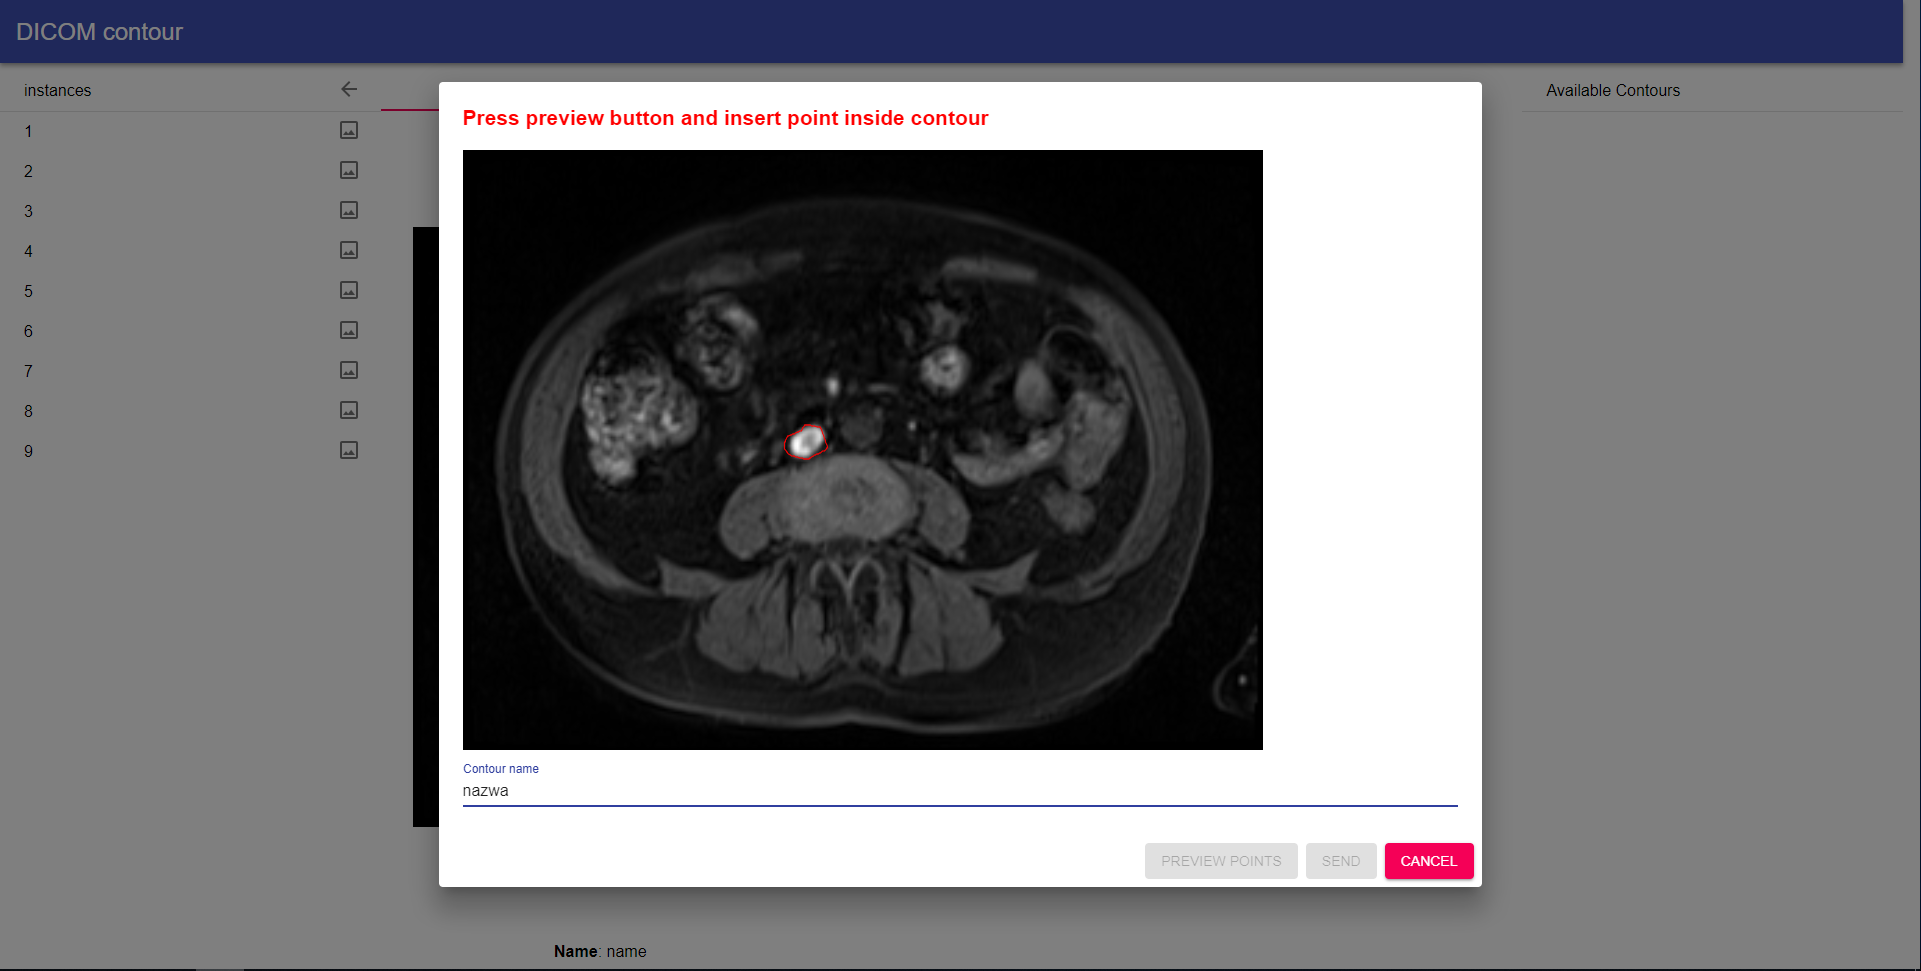
\includegraphics[width=0.48\textwidth]{7}
	\caption{Podgląd wykonanego obrysu}
    	\label{fig:7}
\end{figure}

Następną czynnością, którą musi wykonać użytkownik przed zapisaniem to~wybranie
punktu wewnątrz wykonanego obrysu, poprzez wciśnięcie lewego przycisku myszy w
odpowiednim miejscu na~obrazie --- Rysunek \ref{fig:8}.

\pagebreak

\begin{figure}[h!]
	\center
	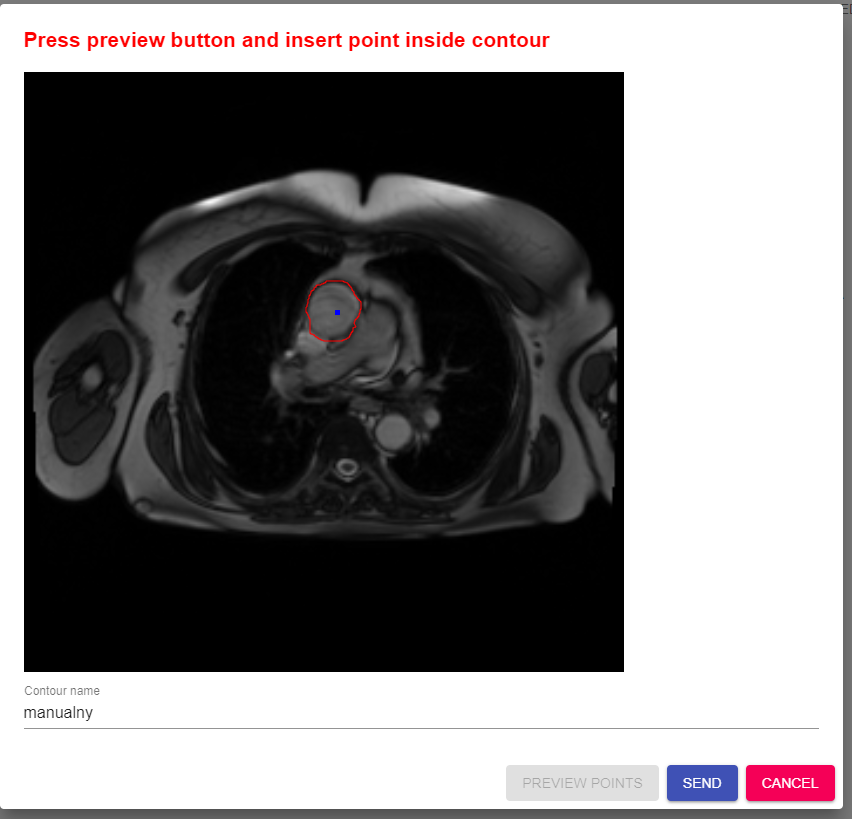
\includegraphics[width=0.6\textwidth]{8}
	\caption{Wybór punktu wewnątrz obrysu}
    	\label{fig:8}
\end{figure}

Po kliknięciu przycisku wyślij (Send) lewym przyciskiem myszy obrys zostaje
zapisany i~pojawia się na~liście wykonanych obrysów (Avaiable Contours). Lista
zawiera jedynie obrysy dla oglądanego obrazu --- Rysunek \ref{fig:9}. Na liście
obrysy pojawiają się w postaci nazwy podanej przy zapisywaniu.

\begin{figure}[h!]
	\center
	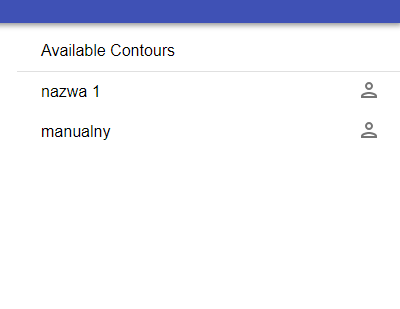
\includegraphics[width=0.35\textwidth]{9}
	\caption{Widok listy obrysów po~zapisaniu obrysu manualnego}
    	\label{fig:9}
\end{figure}

Użytkownik może wykonywać obrysy w~sposób półautomatyczny. W~tym celu musi
wybrać kartę z~obrysami półautomatycznymi (z Manual do~Semi-Automatic) ---
Rysunek \ref{fig:10}. Widok jest bardzo podobny do widoku obrysów manualnych.

\pagebreak

\begin{figure}[h!]
	\center
	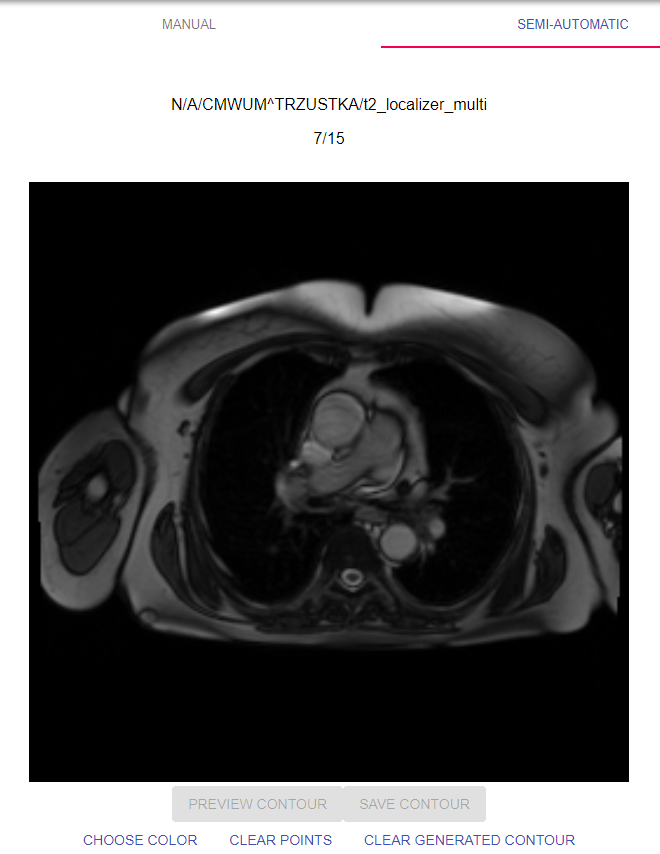
\includegraphics[width=0.4\textwidth]{10}
	\caption{Moduł obrysu półautomatycznego}
    	\label{fig:10}
\end{figure}

Aby wybrać punkty do~obrysu półautomatycznego użytkownik powinien klikać w
interesujące go~punkty lewym przyciskiem myszy. Jeśli korzysta z~tabletu
graficznego, powinien przycisnąć rysik do~tabletu w~interesujących go~punktach.
Punkty wprowadzane powinny być w~kolejności, w~której występują w~obrysie,
zgodnie albo przeciwnie do~ruchu wskazówek zegara --- Rysunek \ref{fig:11}.

\begin{figure}[h!]
	\center
	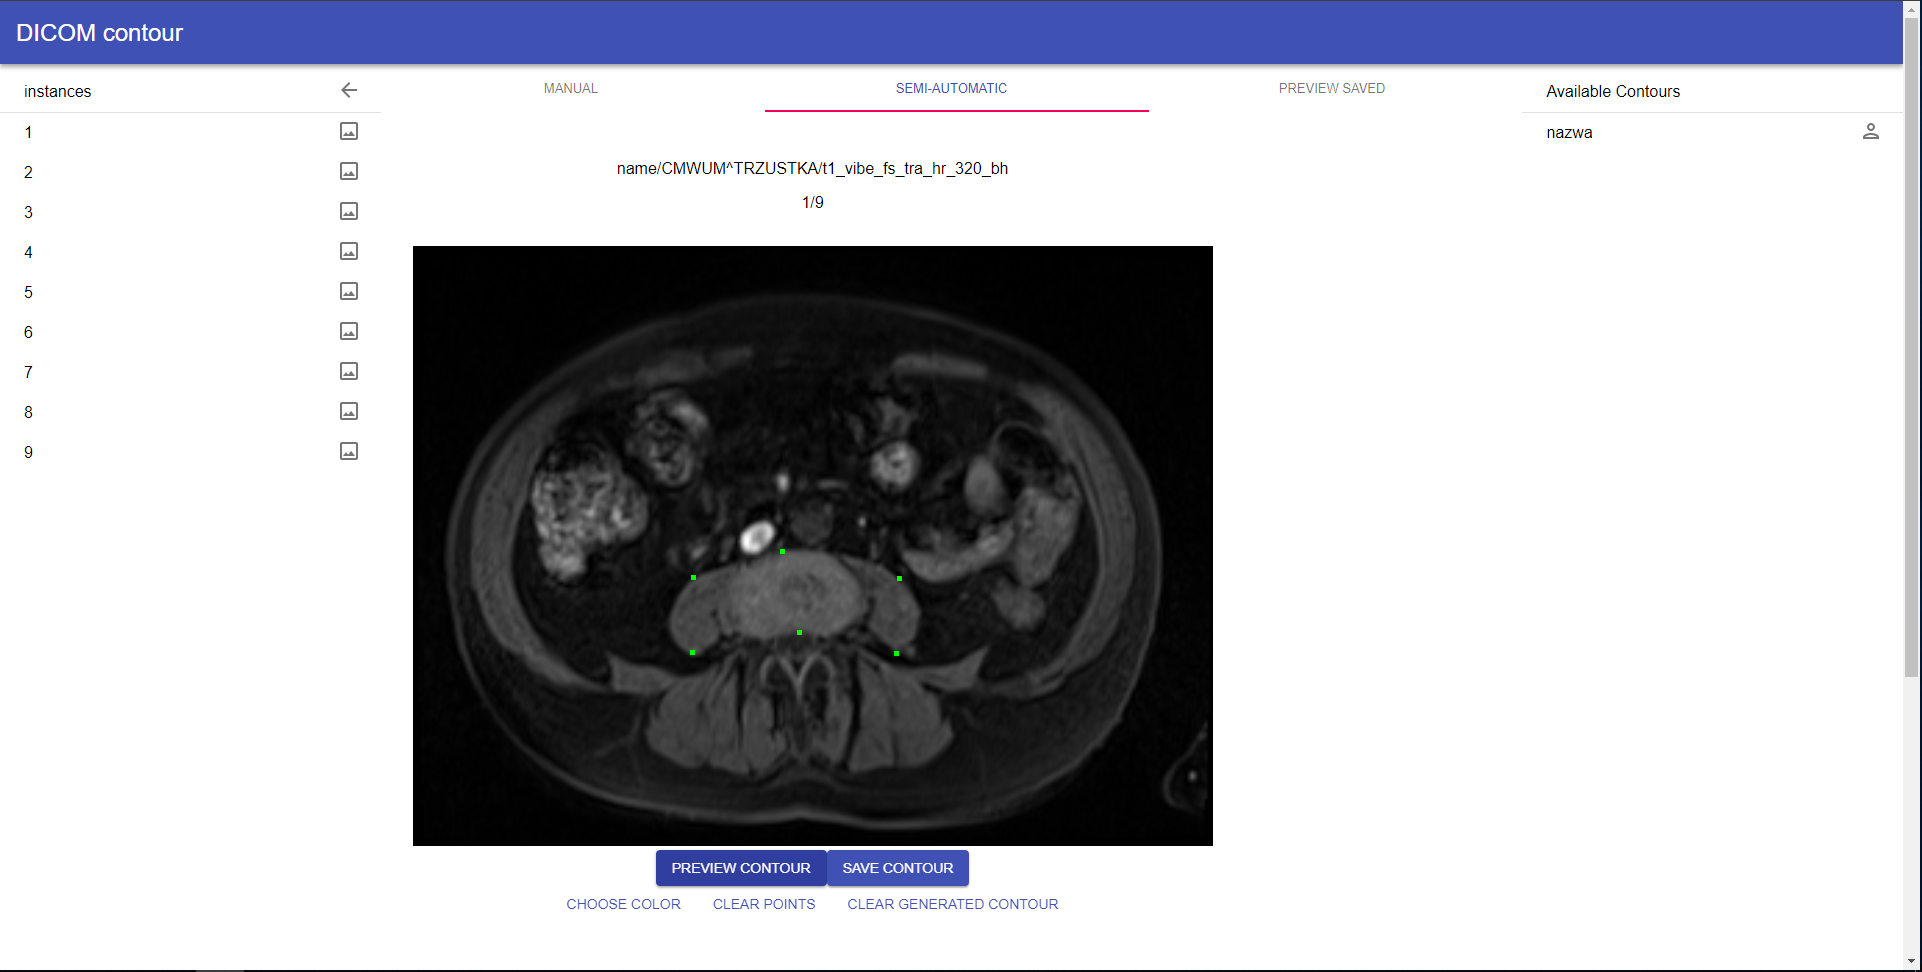
\includegraphics[width=0.4\textwidth]{11}
	\caption{Punkty wybrane do~obrysu półautomatycznego}
    	\label{fig:11}
\end{figure}

\pagebreak

Po wciśnięciu przycisku podgląd obrysu (Preview Contour) użytkownik może
zobaczyć wygenerowany przez algorytm obrys. --- Rysunek \ref{fig:12}.

\begin{figure}[h!]
	\center
	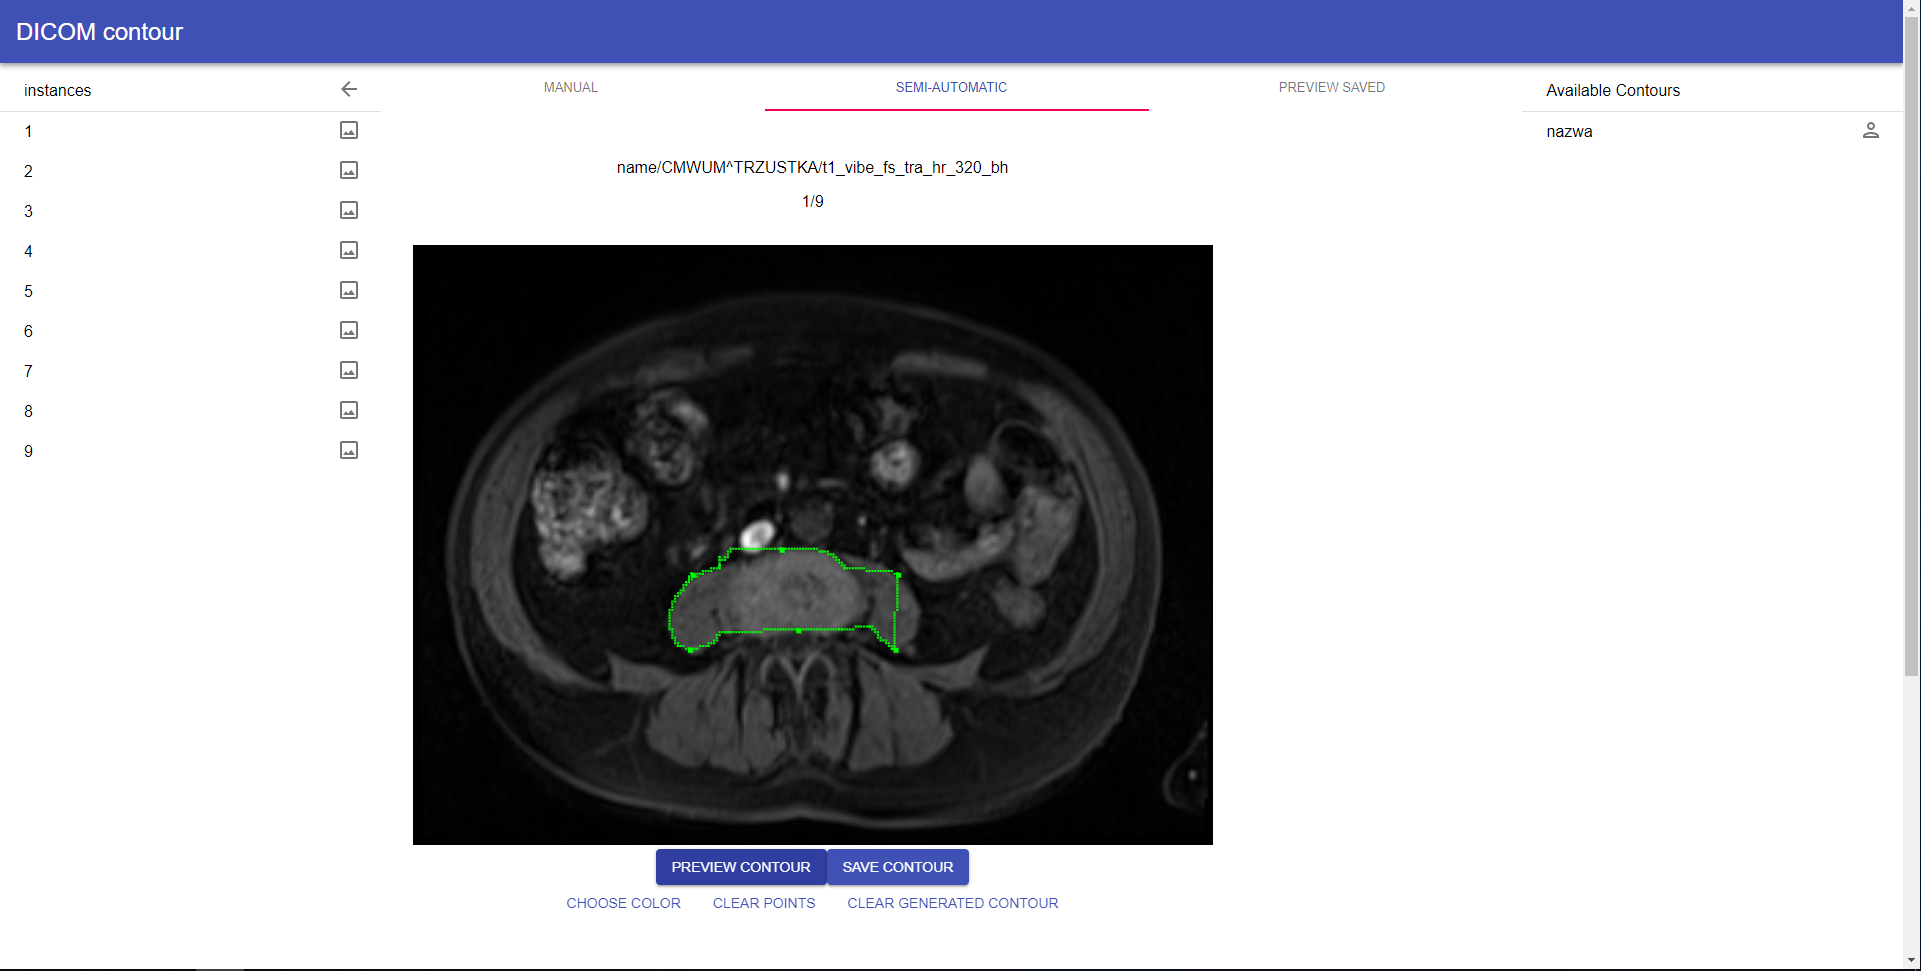
\includegraphics[width=0.5\textwidth]{12}
	\caption{Podgląd obrysu półautomatycznego}
    	\label{fig:12}
\end{figure}

Jeśli algorytm popełnił błąd użytkownik może dodać nowe punkty klikając lewym
przyciskiem myszy w~interesujących go~miejscach lub usunąć nietrafnie umieszczone
punkty poprzez klikanie na~nich lewego przycisku myszy --- Rysunek \ref{fig:13}.

\begin{figure}[h!]
	\center
	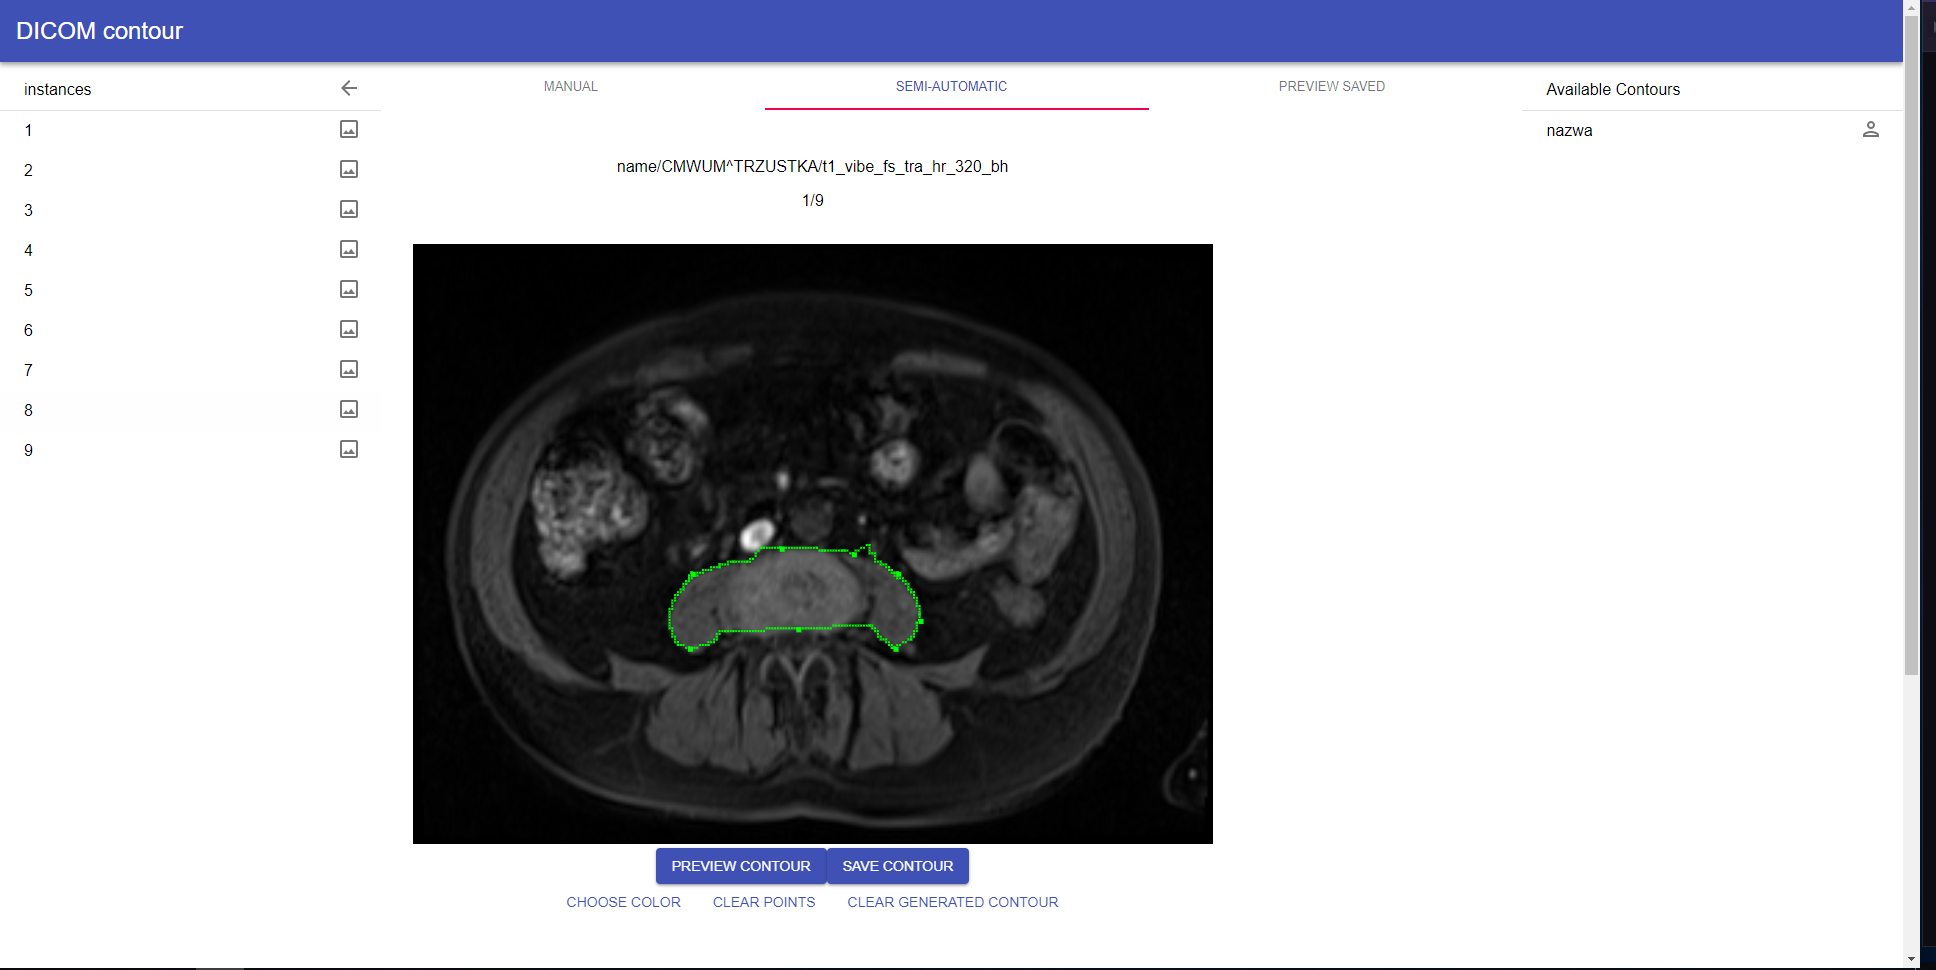
\includegraphics[width=0.5\textwidth]{13}
	\caption{Podgląd obrysu półautomatycznego po~dodaniu nowych punktów}
    	\label{fig:13}
\end{figure}

\pagebreak

Gdy wygenerowany obrys jest satysfakcjonujący dla użytkownika, może on~go~zapisać
klikając przycisk zapisz obrys (Save Contour). Okno zapisu jest analogiczne do~okna zapisu
obrysu manualnego. Jeśli na~obrazie pojawią się krzyżujące krawędzie, należy
wyczyścić obrys i~wykonać go~od~początku, gdyż algorytm modyfikujący obrys dodał
nowe punkty w~złym miejscu lub użytkownik wprowadził punkty w~złej kolejności
--- Rysunek \ref{fig:14}.

\begin{figure}[h!]
	\center
	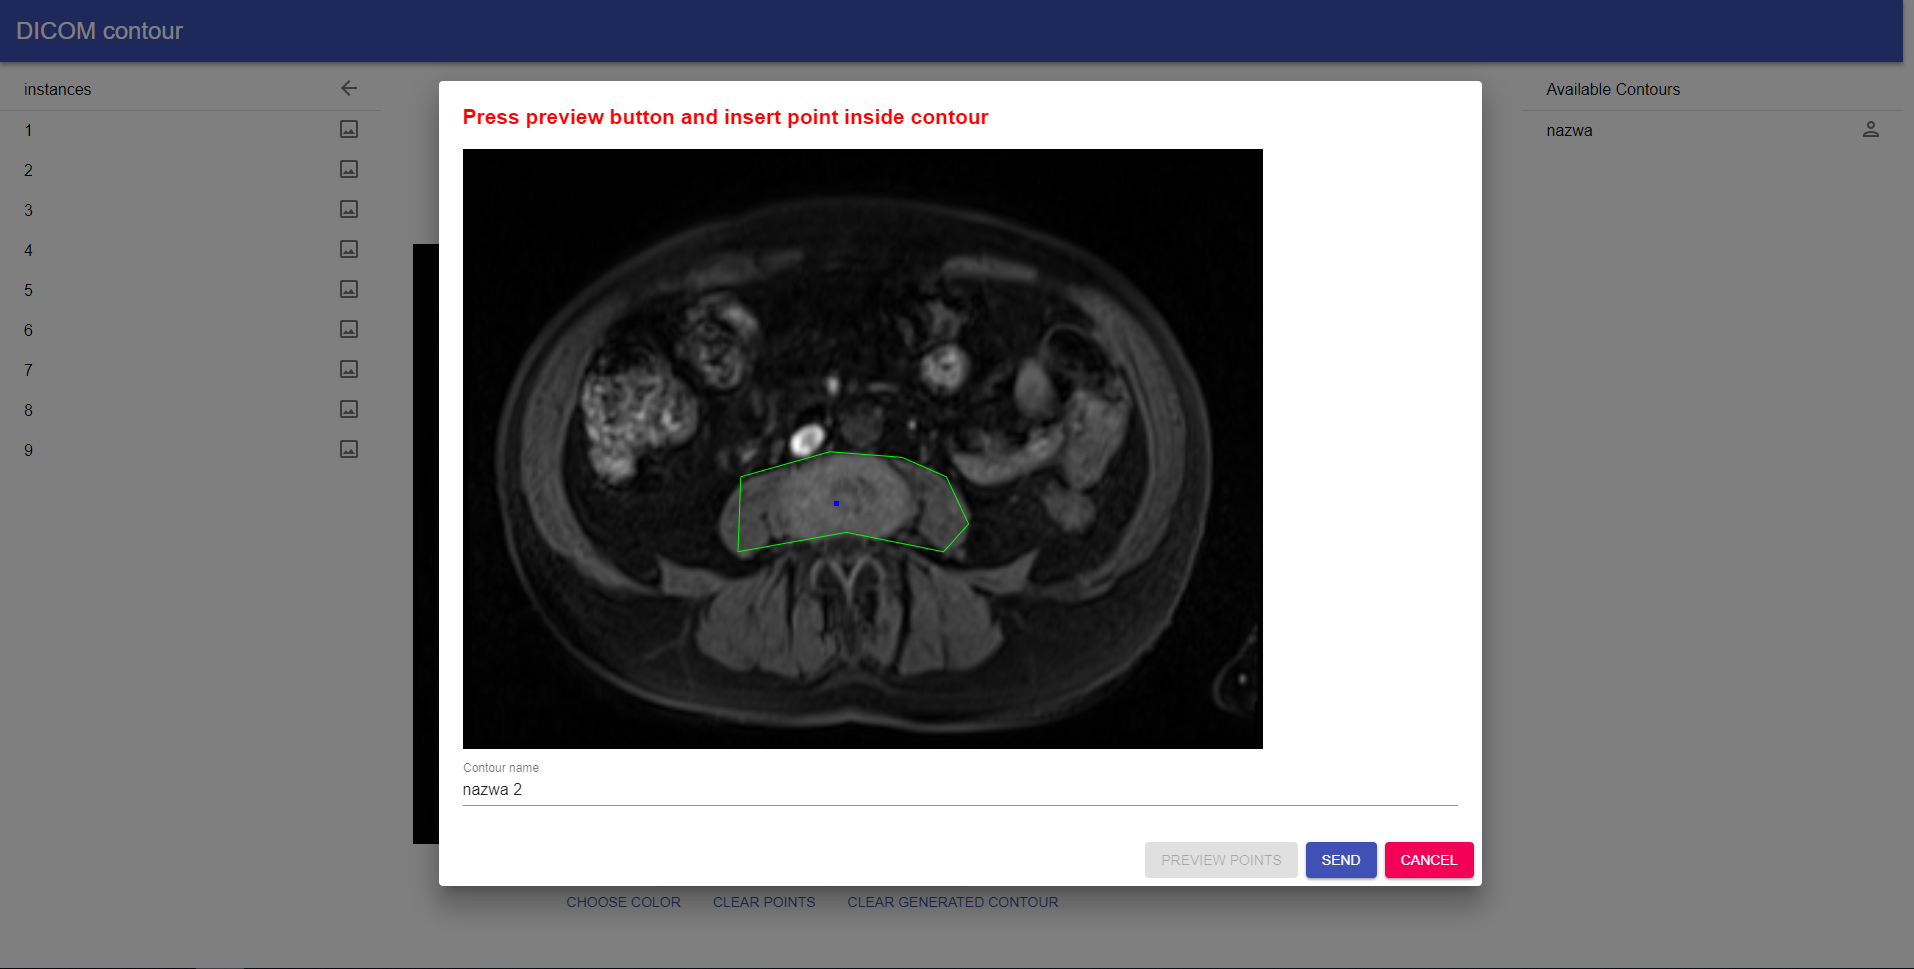
\includegraphics[width=0.5\textwidth]{14}
	\caption{Widok zapisu obrysu półautomatycznego}
    	\label{fig:14}
\end{figure}

Po zapisaniu użytkownik może obejrzeć statystyki wykonanego obrysu poprzez
kliknięcie lewego przycisku myszy na~nazwie obrysu --- Rysunek \ref{fig:15}.

\begin{figure}[h!]
	\center
	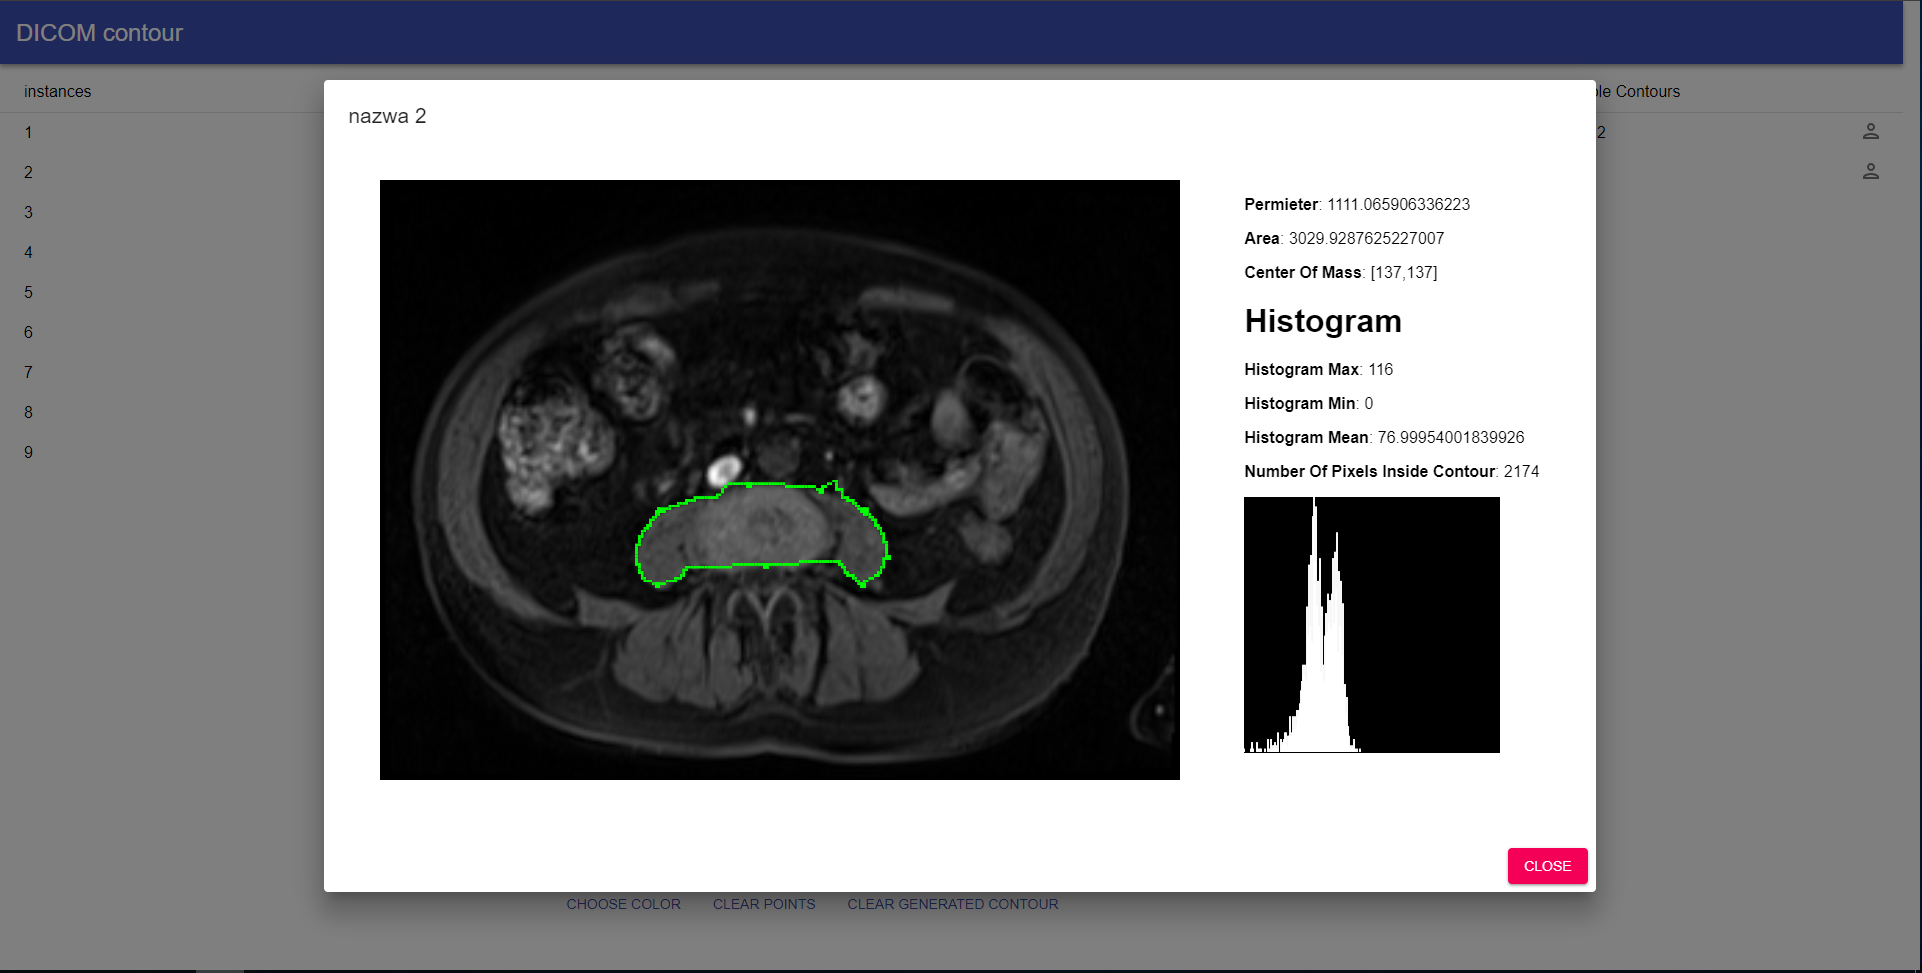
\includegraphics[width=0.5\textwidth]{15}
	\caption{Podgląd statystyk obrysu}
    	\label{fig:15}
\end{figure}

\pagebreak

Przed wykonaniem obrysu użytkownik może wybrać kolor wykonywanego obrysu.
Po wciśnięciu lewym przyciskiem myszy na~przycisk wybierz kolor (Choose Color),
pojawia się okno wyboru koloru. Użytkownik może wybrać kolor z~przygotowanej
wcześniej palety kolorów lub wprowadzić dowolny inny korzystając z~pól tekstowych,
wprowadzając kod RGB wybranego koloru --- Rysunek \ref{fig:16}.

\begin{figure}[h!]
	\center
	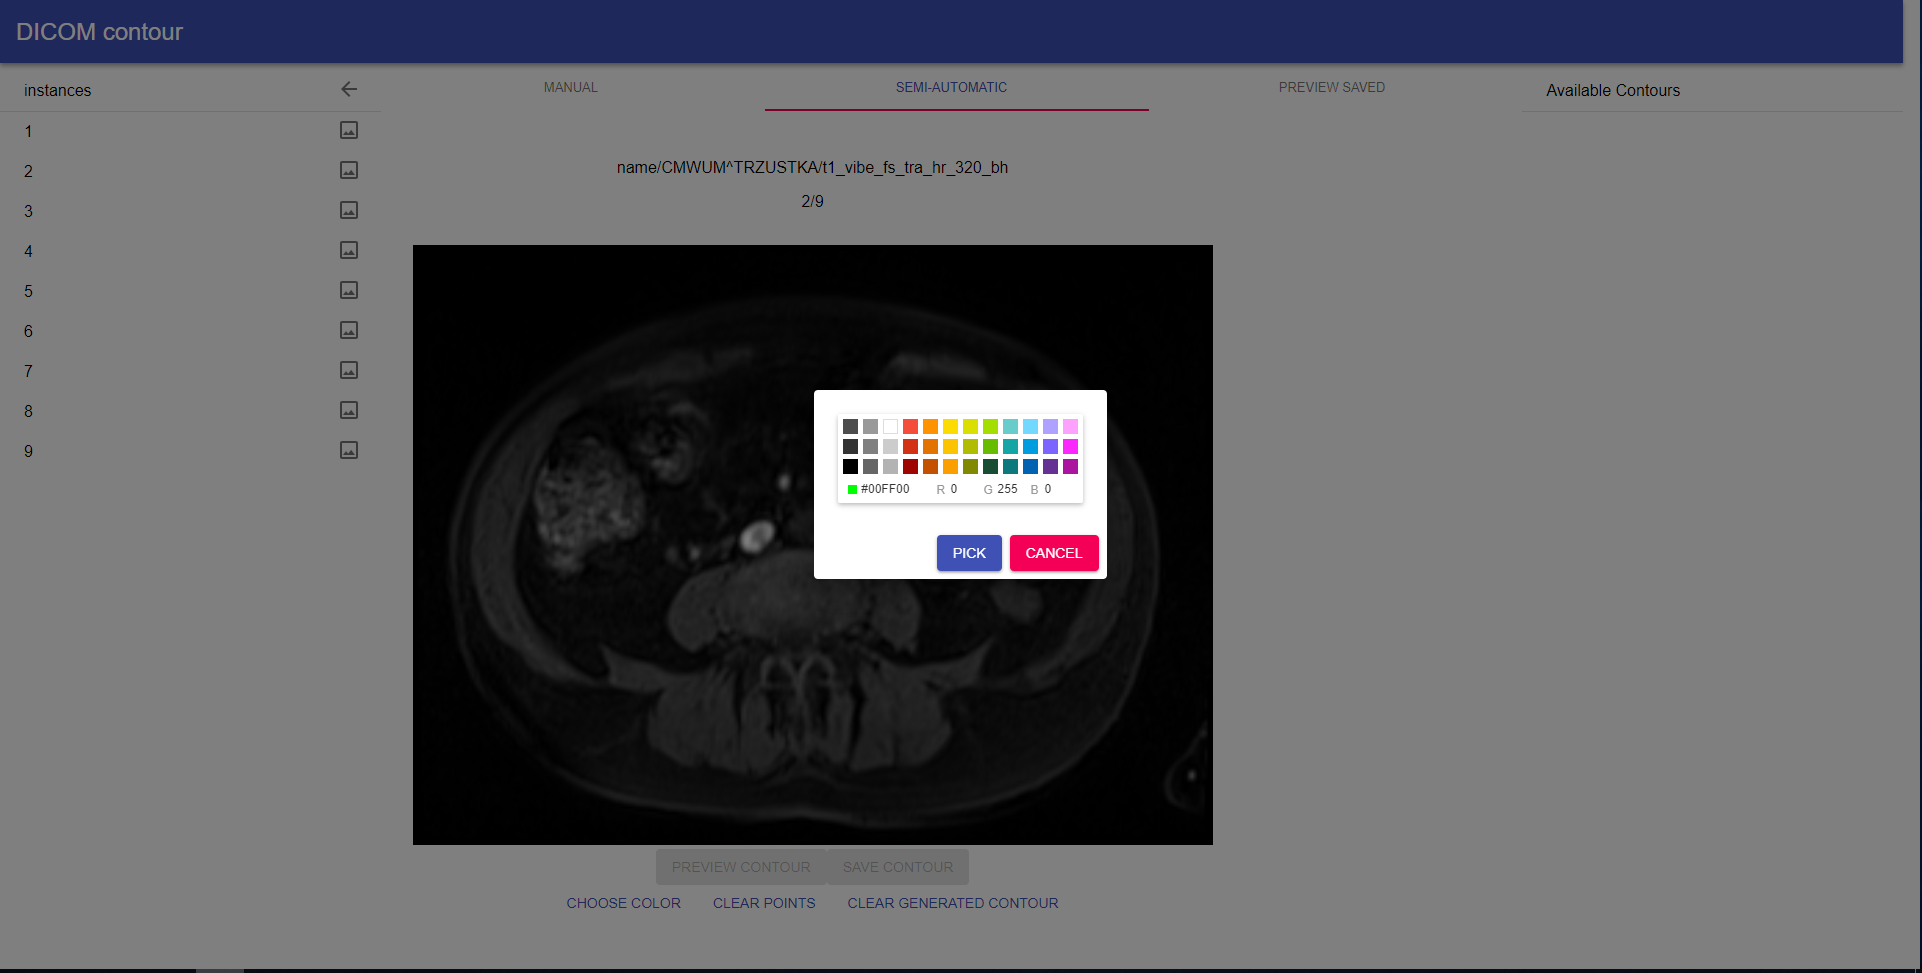
\includegraphics[width=0.35\textwidth]{16}
	\caption{Widok wyboru koloru obrysu}
    	\label{fig:16}
\end{figure}

W zakładce z~podglądem obrysów użytkownik może wyświetlać wybrane przez niego
obrysy z~listy wykonanych obrysów. Użytkownik wybiera obrysy, które chce zobaczyć.
Obrysy, które nie są aktualnie wyświetlane można dodać do~obrazu klikając je
lewym przyciskiem myszy na~nazwie obrysu, a~wyświetlane można wyłączyć również
poprzez kliknięcie lewego przycisku myszy na~nazwie obrysu --- Rysunek \ref{fig:17}.

\begin{figure}[h!]
	\center
	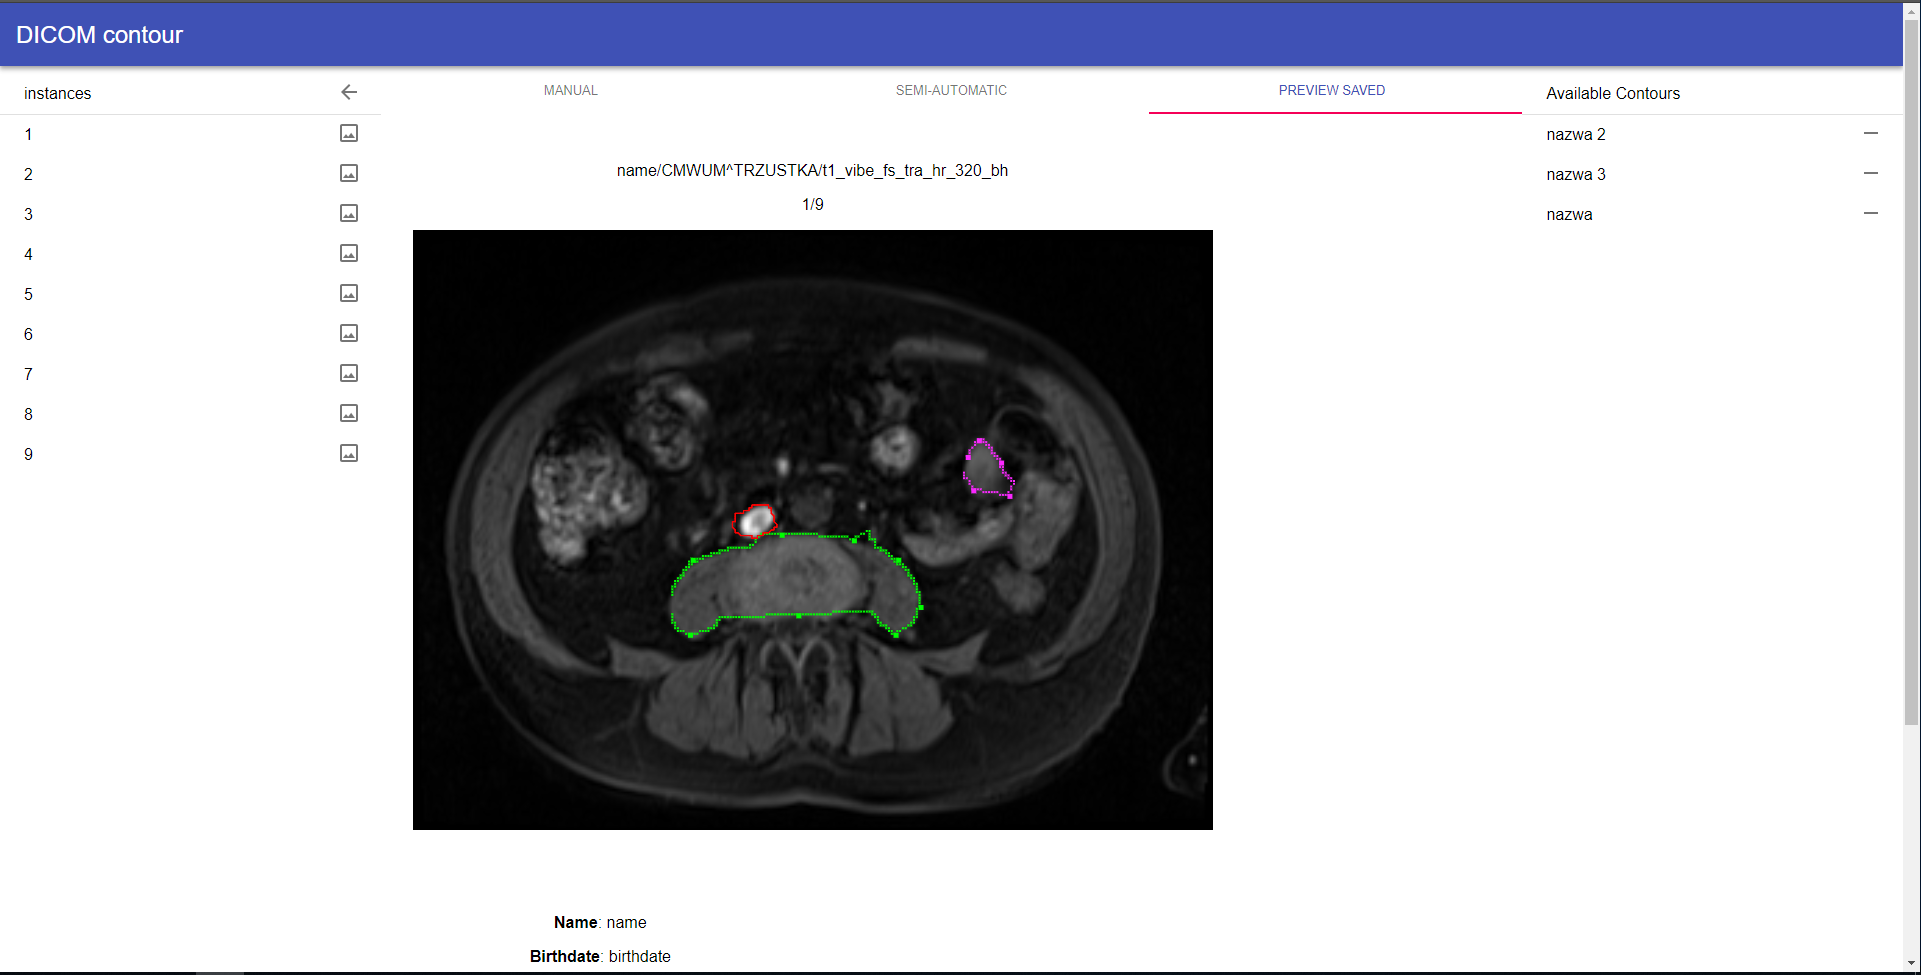
\includegraphics[width=0.6\textwidth]{17}
	\caption{Widok wielu obrysów}
    	\label{fig:17}
\end{figure}

\pagebreak

Interfejs wyświetla również informacje dotyczące pacjenta i~jego badania oraz
wyświetlanego obrazu --- Rysunek \ref{fig:18}.

\begin{figure}[h!]
	\center
	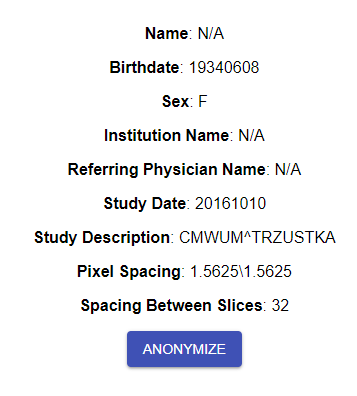
\includegraphics[width=0.4\textwidth]{18}
	\caption{Widok szczegółów obrazu}
    	\label{fig:18}
\end{figure}

Poprzez wciśnięcie przycisku anonimizuj (Anonymize) użytkownik może wybrać nazwę
pacjenta, datę jego urodzenia oraz płeć po~anonimizacji jego danych --- Rysunek \ref{fig:19}.

\begin{figure}[h!]
	\center
	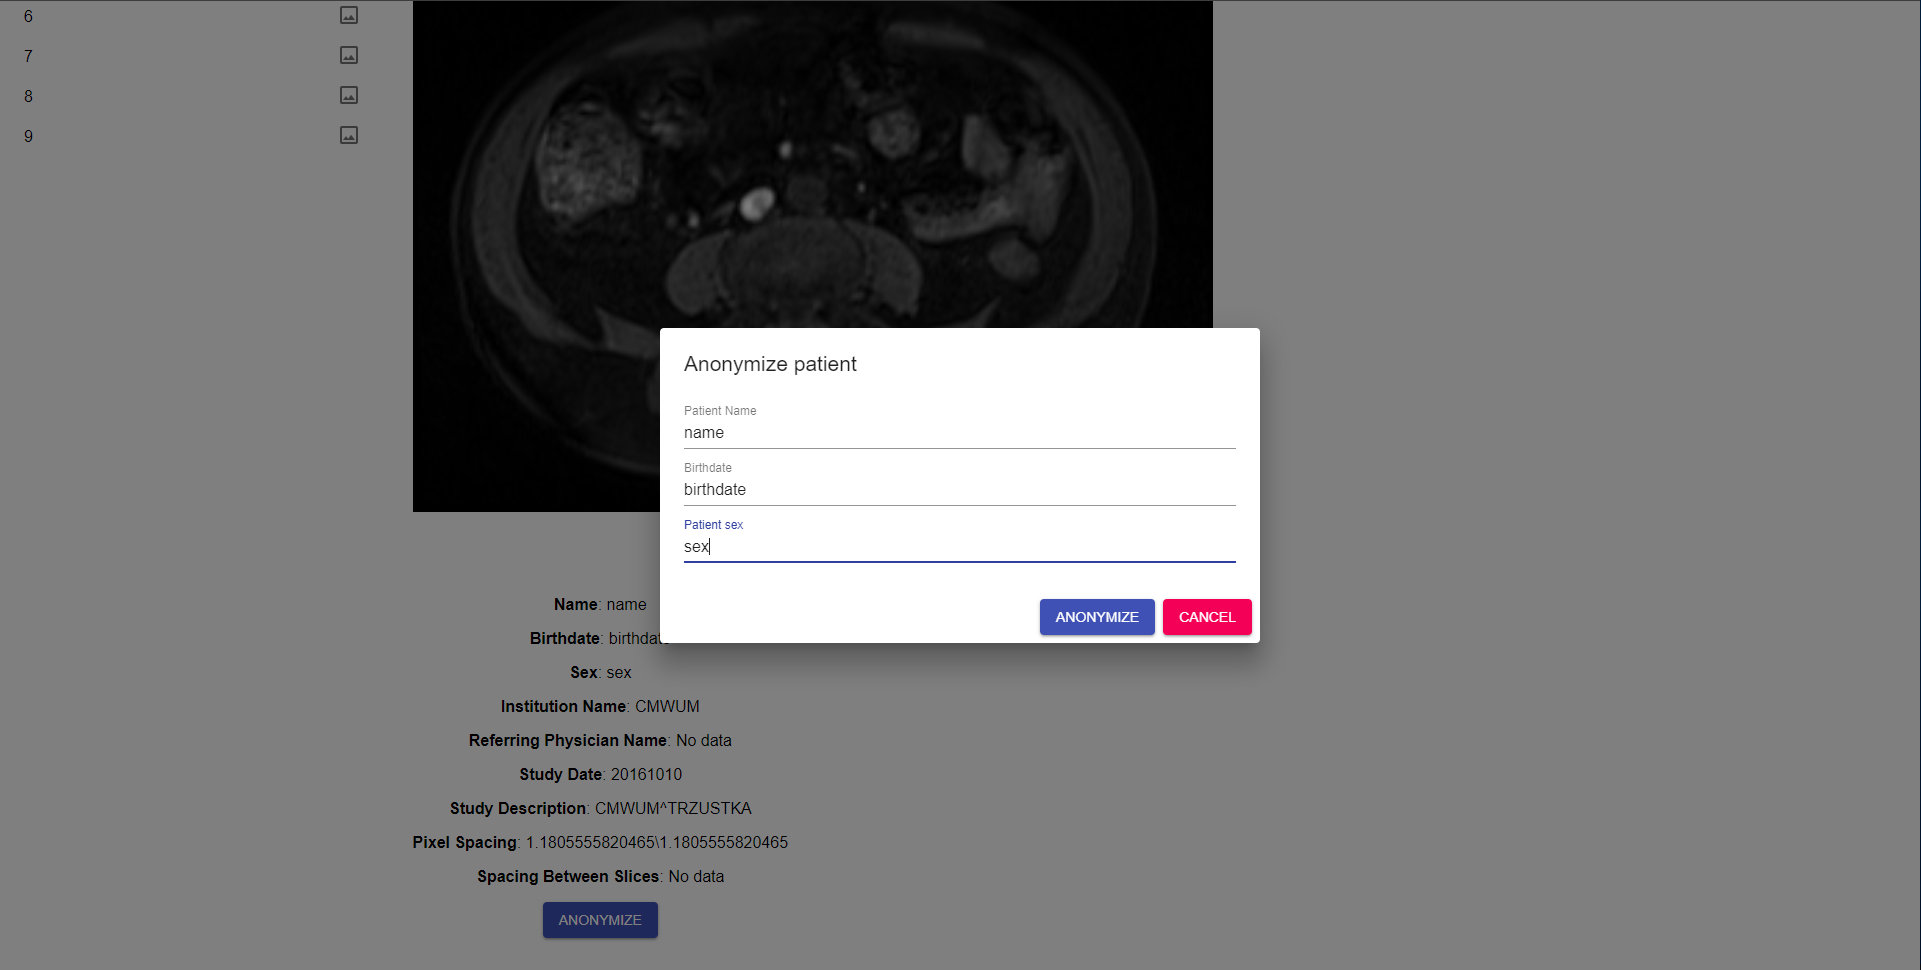
\includegraphics[width=0.6\textwidth]{19}
	\caption{Anonimizacja danych pacjenta}
    	\label{fig:19}
\end{figure}



%\end{enumerate}
%\thispagestyle{empty}

\end{document}
